\documentclass[11pt]{article} 
%\documentclass[9pt,twocolumn,twoside]{pnas-new}
%\documentclass[9pt,twocolumn,pnasresearcharticle]{pnas-new}
%\documentclass[9pt,twocolumn,twoside]{pnas-new}
% Use the lineno option to display guide line numbers if required.

\usepackage{booktabs}

\newcommand\arxiv[2]{#1} % 1st argument for arxiv format
% \newcommand\arxiv[2]{#2} % 2nd argument for PNAS format
% also, swich to \documentclass[11pt]{article} for arxiv format

%%%%% NEW MATH DEFINITIONS %%%%%
\usepackage{amsmath,bbm,bm}
\usepackage{amssymb}
\usepackage{amsfonts}
\usepackage{amsthm}
\usepackage{mathtools}

% commands
% global count (no section number)
\newtheorem{thm}{Theorem}%[section]
\newtheorem{lem}{Lemma}
\newtheorem{prop}{Proposition}
\newtheorem{cor}{Corollary}
\newtheorem{conj}{Conjecture}
\newtheorem{aspt}{Assumption}
\newtheorem{claim}{Claim}
\newtheorem{rmk}{Remark}
\newtheorem{commt}{Comment}
\newtheorem{defn}{Definition}

% algorithm
%\usepackage{algorithm, algorithmic}
%\usepackage{algorithm2e}
\usepackage{tabularx}
%\usepackage[table,xcdraw]{xcolor}

% Comments
% \usepackage{xcolor} % already loaded
\newcount\comments  % 0 suppresses notes to selves in text
\comments=1  % TODO: change to 0 for final version
\newcommand{\genComment}[2]{\ifnum\comments=1{\textcolor{#1}{\textsf{\footnotesize #2}}}\fi}
\newcommand{\ed}[1]{\genComment{red}{[EI:#1]}}
\newcommand{\giles}[1]{\genComment{green}{[GH:#1]}}
\newcommand{\kevin}[1]{\genComment{blue}{[KT:#1]}}


% Mark sections of captions for referring to divisions of figures
\newcommand{\figleft}{{\em (Left)}}
\newcommand{\figcenter}{{\em (Center)}}
\newcommand{\figright}{{\em (Right)}}
\newcommand{\figtop}{{\em (Top)}}
\newcommand{\figbottom}{{\em (Bottom)}}
\newcommand{\captiona}{{\em (a)}}
\newcommand{\captionb}{{\em (b)}}
\newcommand{\captionc}{{\em (c)}}
\newcommand{\captiond}{{\em (d)}}


\newcommand\seq[2]{{#1}\!:\!{#2}}
\newcommand\R{\mathbb{R}}
\newcommand\Var{\mathrm{Var}}
\newcommand\var{\Var}
\newcommand\Cov{\mathrm{Cov}}
\newcommand\cov{\Cov}
\newcommand\iid{\mathrm{iid}}
\newcommand\dist{d}
\newcommand\lik{\mathcal{L}}
\newcommand\prob{\mathbb{P}}
\newcommand\E{\mathbb{E}}
\newcommand\loglik{\ell}
\newcommand\process{\texttt{process}}
\newcommand\dimtheta{\mathrm{dim}_{\Theta}}
\newcommand\param{\,;}
\newcommand\giventh\param
\newcommand\given{{\,\vert\,}}
\newcommand\code[1]{\texttt{#1}}
\newcommand\ceil[1]{\lceil #1 \rceil}
\newcommand\floor[1]{\lfloor #1 \rfloor}
\newcommand\1{\bm{1}}


% Highlight a newly defined term
\newcommand{\newterm}[1]{{\bf #1}}


% Figure reference, lower-case.
\def\figref#1{figure~\ref{#1}}
% Figure reference, capital. For start of sentence
\def\Figref#1{Figure~\ref{#1}}
\def\twofigref#1#2{figures \ref{#1} and \ref{#2}}
\def\quadfigref#1#2#3#4{figures \ref{#1}, \ref{#2}, \ref{#3} and \ref{#4}}
% Section reference, lower-case.
\def\secref#1{section~\ref{#1}}
% Section reference, capital.
\def\Secref#1{Section~\ref{#1}}
% Reference to two sections.
\def\twosecrefs#1#2{sections \ref{#1} and \ref{#2}}
% Reference to three sections.
\def\secrefs#1#2#3{sections \ref{#1}, \ref{#2} and \ref{#3}}
% Reference to an equation, lower-case.
\def\eqref#1{equation~\ref{#1}}
% Reference to an equation, upper case
\def\Eqref#1{Equation~\ref{#1}}
% A raw reference to an equation---avoid using if possible
\def\plaineqref#1{\ref{#1}}
% Reference to a chapter, lower-case.
\def\chapref#1{chapter~\ref{#1}}
% Reference to an equation, upper case.
\def\Chapref#1{Chapter~\ref{#1}}
% Reference to a range of chapters
\def\rangechapref#1#2{chapters\ref{#1}--\ref{#2}}
% % Reference to an algorithm, lower-case.
% \def\algref#1{algorithm~\ref{#1}}
% % Reference to an algorithm, upper case.
% \def\Algref#1{Algorithm~\ref{#1}}
% \def\twoalgref#1#2{algorithms \ref{#1} and \ref{#2}}
% \def\Twoalgref#1#2{Algorithms \ref{#1} and \ref{#2}}
% Reference to a part, lower case
\def\partref#1{part~\ref{#1}}
% Reference to a part, upper case
\def\Partref#1{Part~\ref{#1}}
\def\twopartref#1#2{parts \ref{#1} and \ref{#2}}

\def\eps{{\epsilon}}

\def\gN{{\mathcal{N}}}
\def\gX{{\mathcal{X}}}
\def\gY{{\mathcal{Y}}}


\makeatletter
\newcommand*{\addFileDependency}[1]{% argument=file name and extension
\typeout{(#1)}% latexmk will find this if $recorder=0
% however, in that case, it will ignore #1 if it is a .aux or 
% .pdf file etc and it exists! If it doesn't exist, it will appear 
% in the list of dependents regardless)
%
% Write the following if you want it to appear in \listfiles 
% --- although not really necessary and latexmk doesn't use this
%
\@addtofilelist{#1}
%
% latexmk will find this message if #1 doesn't exist (yet)
\IfFileExists{#1}{}{\typeout{No file #1.}}
}\makeatother

\newcommand*{\myexternaldocument}[1]{%
\externaldocument{#1}%
\addFileDependency{#1.tex}%
\addFileDependency{#1.aux}%
}

\usepackage{tabto}

\arxiv{
  \usepackage{fullpage}
  %% some packages loaded by pnas-new.cls which we need for
  %% the arxiv version
  \usepackage{algorithm}
  \usepackage[noend]{algpseudocode}
  \usepackage{xcolor}
  \usepackage{tikz}
  \usepackage{enumitem}
  \bibliographystyle{ieeetr}
}{
\templatetype{pnasresearcharticle} % Choose template
% {pnasresearcharticle} = Template for a two-column research article
% {pnasmathematics} %= Template for a one-column mathematics article
% {pnasinvited} %= Template for a PNAS invited submission
}

\begin{document}

\title{Accelerated Inference for Partially Observed Markov Processes using Automatic Differentiation}

%\arxiv{ \author{K. Tan, G. Hooker and E. L. Ionides\\
%  \small{Department of Statistics, University of Pennsylvania}\\
%  \small{Department of Statistics, University of Michigan}}}{}

\arxiv{ \author{K. Tan$^{1}$, G. Hooker$^{1}$ and E. L. Ionides$^{2}$
  \vspace{2mm}\\
  \small{$^{1}$Department of Statistics, University of Pennsylvania}\\
  \small{$^{2}$Department of Statistics, University of Michigan}}}{}

\arxiv{}{
% Use letters for affiliations, numbers to show equal authorship (if applicable) and to indicate the corresponding author
\author[a]{Kevin Tan}
\author[a]{Giles Hooker}
\author[b,1]{Edward L. Ionides}
%\author[a]{Author Three}
\affil[a]{University of Pennsylvania}
\affil[b]{University of Michigan}
%\affil[c]{Affiliation Three}
% Please give the surname of the lead author for the running footer
\leadauthor{Tan}
% Please add a significance statement to explain the relevance of your work
\significancestatement{Many scientific models involve highly nonlinear stochastic dynamical systems which can be observed only via noisy and incomplete measurements. Prior to this work, iterated filtering algorithms were the only class of algorithms for maximum likelihood estimation that did not require access to the system's transition probabilities, instead needing only a simulator of the system dynamics. We leverage recent advances in automatic differentiation to propose a hybrid algorithm that requires only a differentiable simulator for maximum likelihood estimation. Our new method outperforms previous approaches on a challenging problem in epidemiology.}
\authorcontributions{K.T. and E.L.I. designed research; K.T. analyzed data; K.T., G.H. and E.L.I. performed research, K.T., G.H., and E.L.I. wrote the manuscript.}
\authordeclaration{The authors declare no competing interests.}
\correspondingauthor{\textsuperscript{1}To whom correspondence should be addressed. E-mail: kevtan@wharton.upenn.edu}
% At least three keywords are required at submission. Please provide three to five keywords, separated by the pipe symbol.
\keywords{Sequential Monte Carlo $|$ Automatic Differentiation $|$ Particle Filter $|$ Markov Process $|$ Maximum Likelihood}
}

\arxiv{\date{Draft compiled on \today}}{
\dates{This manuscript was compiled on \today}
\doi{\url{www.pnas.org/cgi/doi/10.1073/pnas.XXXXXXXXXX}}
}

\maketitle

\begin{abstract}
  Automatic differentiation (AD) has driven recent advances in machine learning, including deep neural networks and Hamiltonian Markov Chain Monte Carlo methods. Partially observed nonlinear stochastic dynamical systems have proved resistant to AD techniques because widely used particle filter algorithms yield an estimated likelihood function that is discontinuous as a function of the model parameters.  We show how to embed two existing AD particle filter methods in a theoretical framework that provides an extension to a new class of algorithms.  This new class permits a bias/variance tradeoff and hence a mean squared error substantially lower than the existing algorithms. We develop likelihood maximization algorithms suited to the Monte Carlo properties of the AD gradient estimate. Our algorithms require only a differentiable simulator for the latent dynamic system; by contrast, most previous approaches to AD likelihood maximization for particle filters require access to the system's transition probabilities. Numerical results indicate that a hybrid algorithm that uses AD to refine a coarse solution from an iterated filtering algorithm show substantial improvement on current state-of-the-art methods for a challenging scientific benchmark problem.
\end{abstract}

\arxiv{}{
\thispagestyle{firststyle}
\ifthenelse{\boolean{shortarticle}}{\ifthenelse{\boolean{singlecolumn}}{\abscontentformatted}{\abscontent}}{}
\firstpage{4}
% Use \firstpage to indicate which paragraph and line will start the second page and subsequent formatting. In this example, there are a total of 11 paragraphs on the first page, counting the first level heading as a paragraph. The value {12} represents the number of the paragraph starting the second page. If a paragraph runs over onto the second page, include a bracket with the paragraph line number starting the second page, followed by the paragraph number in curly brackets, e.g. "\firstpage[4]{11}".
}

\arxiv{Many}{\dropcap{M}any}
scientific models involve highly nonlinear stochastic dynamic systems possessing significant random variation in both the process dynamics and the measurements.
Commonly, the latent system is modeled as a Markov process, giving rise to a partially observed Markov process (POMP) model, also known as a hidden Markov models or a state space model.
POMP models arise in fields as diverse as automated control \cite{singh22}, epidemiology \cite{he10, stocks17}, ecology \cite{knape12} and finance \cite{kim08, breto14}.
Despite their ubiquity, estimation and inference within this broad class of models remains a challenging problem.
This article concerns the use automatic differentiation (AD) to construct improved algorithms for inference on complex POMP models.

The particle filter, also known as sequential Monte Carlo, serves as the foundation for various inference algorithms for POMP models.
It provides an unbiased estimate of the likelihood function  \cite{delMoral04}, enabling Bayesian inference \cite{andrieu10,chopin13} and likelihood-based inference \cite{ionides06-pnas,ionides15}.
Likelihood-based inference is statistically efficient \cite{pawitan01} and is robust to a moderate amount of Monte Carlo error \cite{ionides17,ning21}.
An attractive feature of basic particle filter algorithms, also known as boostrap filters, is that they do not require evaluation of the transition density of the latent Markov process, enabling an arbitrary model simulator to be plugged into the algorithm.
This plug-and-play property is useful for scientific applications \cite{he10}.
Some plug-and-play methods depend on the construction of low-dimensional summary statistics \cite{wood10,toni09}, sacrificing statistical efficiency for computational convenience.
Plug-and-play methods are often called likelihood-free \cite{owen15}, and it may be counter-intuitive that likelihood-based inference is possible using likelihood-free methods. 
However, iterated filtering algorithms have shown that this is practical in various scientific investigations, such as \cite{king08,blake14,pons-salort18,subramanian21,fox22,drake23}.
Nevertheless, the Monte Carlo variability arising in iterated filtering applications becomes increasingly problematic as the size of the data and the complexity of the model increases.
Algorithmic advances are needed to make plug-and-play likelihood maximization for POMP models more numerically efficient.
We develop plug-and-play AD methods which provide a large computational advantage over the methods used in these previous applications.


Recent advances in AD for particle filters \cite{naesseth18, jonschkowski18, corenflos21, scibior21, singh22} have drawn attention to AD as a tool for inference in POMP models.
However, existing approaches are either asymptotically biased \cite{naesseth18, jonschkowski18}, have high variance \cite{poyiadjis11, scibior21}, are computationally expensive \cite{corenflos21, chen24}, or require access to transition densities \cite{poyiadjis11, scibior21, singh22, chen24}.

Scibior and Wood \cite{scibior21} showed that the estimators derived by Poyiadjis et al. \cite{poyiadjis11} can be attained with standard AD software using an algorithmic procedure, called a {\it stop-gradient}, which allows selected expressions to be evaluated but not differentiated.
Unfortunately, \cite{scibior21} used their estimator within an algorithm which does not have the plug-and-play property and which has high Monte Carlo variability, while the stop-gradient procedure is introduced without mathematical motivation.
We use \cite{scibior21} and \cite{poyiadjis11} as our starting point, while developing a new approach which remedies the weaknesses of these papers.

We start by presenting a new construction of the gradient estimator of \cite{scibior21} and \cite{poyiadjis11}.
Specifically, we show how this estimator can be derived as the direct derivative of a suitably weighted particle filter, which (for reasons which will be discussed later) we call a {\it Measurement Off-Parameter} (MOP) particle filter. 
In short, \textit{instead of directly differentiating through a basic particle filter, MOP uses AD to differentiate through a smooth particle filter constructed using measurement density ratios and a differentiable simulator}. 
Our MOP algorithm differs from previous smooth particle filters \cite{svensson18,malik11} by possessing the plug-and-play property.
Critically, we also avoid the high variance of \cite{svensson18} by generalizing the MOP particle filter to add a discount factor, $\alpha \in [0,1]$.
This discount factor enables MOP-$\alpha$ to interpolate between the  biased gradient estimator of \cite{naesseth18}, when $\alpha=0$, and the high-variance gradient estimate from \cite{poyiadjis11, scibior21}, when $\alpha=1$ (Theorem \ref{thm:mop-functional-forms}).
The bias-variance tradeoff induced by $\alpha$ suggests, both in theory (Theorem \ref{thm:mop-biasvar}) and in practice (Figure \ref{fig:biasvar}), the use of $\alpha$ values strictly between 0 and 1.

MOP-$\alpha$ avoids the issue of asymptotic bias \cite{corenflos21} arising from having to drop terms arising from resampling when differentiating through the standard particle filter as in \cite{naesseth18} in a novel way.
This particle filter is smooth by construction, allowing us to bypass the seemingly incompatible paradox of differentiating through discrete Monte Carlo sampling by instead using AD to differentiate through a series of measurement density ratios and a differentiable simulator.
Yet, MOP-$\alpha$ can nevertheless provide strongly consistent particle and log-likelihood estimates (Theorem \ref{thm:mop-targeting}), and when $\alpha=1$, consistent score estimates (Theorem \ref{thm:mop-grad-consistency}).

We derive a linear convergence rate for stochastic gradient descent (SGD) using MOP-$\alpha$ in the  presence of strong convexity (Theorem \ref{thm:mop-convergence}).
Critically, the estimator converges quickly within a neighborhood of the maximum but struggles to reach this neighborhood in the presence of local minima and saddle points.
That behavior is complementary to that of iterated filtering algorithms \cite{ionides06-pnas,ionides15} which provides a relatively fast and stable way to identify this neighborhood.
We therefore build a simple but effective hybrid algorithm called {\it Iterated Filtering with Automatic Differentiation} (IFAD) that warm-starts first-order or second-order gradient methods with a preliminary solution obtained from a few rounds of iterated filtering.
Promising numerical results indicate that IFAD beats IF2 (and by the numerical results of \cite{ionides15}, also IF1 \cite{ionides06-pnas,ionides11} and the Liu-West filter \cite{liuwest01}) on a challenging problem in epidemiology, the Dhaka cholera model of \cite{king08}.

These improvements also extend to Bayesian inference, as we show in Section \ref{sec:bayes} that we can use the MOP-$\alpha$ gradient estimates within a No-U-Turn Sampler (NUTS) \cite{homan14} in conjunction with a nonparametric empirical Bayes-style prior estimated with IF2 to reduce the burn-in period of particle MCMC \cite{andrieu10} on the Dhaka cholera model of \cite{king08} from the $700,000$ iterations in \cite{fasiolo16} to just $500$. To the best of our knowledge, attaining rapid mixing on this challenging problem has not previously been achievable. 

\section{Problem Setup}

Consider an unobserved Markov process $\{X(t),t  \geq t_0\}$, with discrete-time observations $Y_1,...,Y_N$ realized at values $y_1^*,...,y_N^*$ at times $t_1,..., t_N$.
The process is parameterized by an unknown parameter $\theta \in \Theta \subseteq \R^p$, where the state $X(t)$ take values in the state space $\gX \subseteq \R^d$, the observations $Y_n$ take values in $\gY,$ and we write $X_n := X(t_n)$. 

% By a similar decomposition to that in \cite{doucet2009tutorial}, we find that the joint density of $X_{0:N}, Y_{1:N}$ can be factored as
% \begin{align*}
%     &f_{X_{0: N}, Y_{1: N}}\left(x_{0: N}, y_{1: N} ; \theta\right)\\
%     &=f_{X_0}\left(x_0 ; \theta\right) \prod_{n=1}^N f_{X_n \mid X_{n-1}}\left(x_n \mid x_{n-1} ; \theta\right) f_{Y_n \mid X_n}\left(y_n \mid x_n ; \theta\right).
% \end{align*}

We suppose that the discete-time latent process model has a density $f_{X_n|X_{n-1}}\left(x_{n} \mid x_{n-1}; \theta\right)$.
The existence of this density is necessary to define the likelihood function, but plug-and-play algorithms do not have access to evaluation of this density.
Instead, they have access to a corresponding simulator, which we write as $\process_n\left(x_n\mid x_{n-1}; \theta\right)$.
We set $f_{Y_n|X_n}\left(y_n \mid x_n; \theta\right)$ to be the measurement density, which we suppose can be evaluated. We write $y_n^*$ for the actual values of the observations that were observed.
We call $f_{X_{1:n}|Y_{1:n}}(x_{1:n}|y_{1:n}^*; \theta)$ the posterior distribution of states, and $f_{X_{n}|Y_{1:n}}(x_n|y_{1:n}^*; \theta)$ the filtering distribution at time $t_n$.
Superscripts $x_{n,j}^A$ of particles denote the ancestral trajectory of particle $j$ at time $n$, $a(\cdot)$ is the ancestor function that maps a particle to its parent, $j \mapsto a(j)$, and $k_j$
denotes the resample indices drawn for each particle $j$. 

The above densities are defined on a probability space $(\Omega, \Sigma, \prob)$ which is also assumed to enable construction of independent replicates and all other random variables defined in our algorithms.
For the algorithmic interpretation of our theory, we identify the random number seed with an element of the sample space $\omega \in \Omega$. The random seed determines the sequence of pseudo-random numbers as generated by a computer, just as the outcome $\omega\in\Omega$ generates the sequence of random variables.

%When two algorithms share the same seed, this corresponds to the method of common random numbers. 


\section{Off-Parameter Particle Filters}

%Directly differentiating through a particle filter, for a fixed value of $\omega$, leads to a biased gradient estimator due to the discreteness of the resampling operation \cite{corenflos21}.
Our approach is as follows. \textit{Instead of directly differentiating through a basic particle filter, we instead use AD to differentiate through a series of measurement density ratios and a differentiable simulator}. 
This is done through the construction of a novel particle filtering algorithm called {\it Measurement Off-Parameter with discount factor} $\alpha$ (MOP-$\alpha$), defined by the pseudocode in Algorithm~\ref{alg:mop}.
Note that the plug-and-play property forbids access to transition densities but permits access to the density of the measurements conditional on the value of the latent process.
The simulator can be differentiated using AD as long as the underlying computer code for the simulator is differentiable, and so MOP-$\alpha$ is applicable to a broad class of POMP models.

The MOP-$\alpha$ algorithm resamples the particles according to an arbitrary resampling rule that depends on both the target parameter value and a baseline parameter value, and this explains the name {\it measurement off-parameter}.
This is intended as an analogy to {\it off-policy} learning in reinforcement learning.
Specifically, MOP-$\alpha$ evaluates the likelihood at some $\theta \in \Theta$, but instead resamples the particles according to the indices generated by a vanilla particle filter run at a {\it baseline parameter}, $\phi \in \Theta$.
This ensures that the resampling indices are invariant to $\theta$ when $\omega$ and $\phi$ are fixed, bypassing the issue of Monte Carlo resampling.
We show in Theorem~\ref{thm:mop-targeting} that MOP-$\alpha$ exactly targets the filtering distribution when $\theta=\phi$ or $\alpha=1$.

We suppose that the simulator is a differentiable function of $\theta$ for every fixed $\omega$, a condition that requires the latent process to be a continuous random variable. 
This condition is also known as the {\it reparameterization trick} \cite{corenflos21}.
Supposing also that the measurement model is differentiable in $\theta$, direct differentiation of MOP-$\alpha$ is available via AD.
Theorem~\ref{thm:mop-functional-forms} shows that MOP-$\alpha$ is constructed so this direct derivative obtains the score estimator of  \cite{poyiadjis11, scibior21} when $\alpha=1$ and that of \cite{naesseth18} when $\alpha=0$.
Setting $\alpha<1$ adds bias but reduces variance, raising opportunities for a favorable tradeoff as illustrated in theory (Theorem \ref{thm:mop-biasvar}) and in practice (Figure \ref{fig:biasvar}).


\begin{algorithm}[H]
	\caption{MOP-$\alpha$}
    \label{alg:mop}
	     \textbf{Input:} Number of particles $J$, timesteps $N$, measurement model $f_{Y_n|X_n}(y_n^*|x_n, \theta)$, simulator $\process_n(x_{n+1}|x_n; \theta)$, evaluation parameter $\theta$, behavior parameter $\phi$, seed $\omega$.
      
        \textbf{First pass:} Set $\theta=\phi$ and fix $\omega$, yielding $X_{n,j}^{P,\phi}$, $X_{n,j}^{F,\phi}$, $g^{\phi}_{n,j}$.
            
        \textbf{Second pass:}
        Fix $\omega$, and filter at $\theta\neq \phi$:
            
		\textbf{Initialize } particles ${X}_{0,j}^{F,\theta}\sim {f}_{{X}_{0}}\left(\cdot\giventh{\theta}\right)$, weights $w^{F,\theta}_{0,j}= 1$. \newline
		\textbf{For} $n=1,...,N$: \newline
            \hspace*{4mm} Accumulate discounted weights, $w_{n,j}^{P,\theta} = \big(w_{n-1,j}^{F,\theta}\big)^\alpha$.\newline
            \hspace*{4mm} Simulate process model,
            ${X}_{n,j}^{P,\theta}\sim \process_n\big(\cdot|{X}_{n-1,j}^{F, \theta};{\theta}\big)$. \newline
            \hspace*{4mm} Measurement density,
            $g^{\theta}_{n,j}={f}_{{Y}_{n}|{X}_{n}}(y_{n}^{*}|{X}_{n,j}^{P,\theta}\giventh{\theta})$. \newline
            \hspace*{4mm} Compute $L_n^{B,\theta,\alpha} ={\sum_{j=1}^Jg^\theta_{n,j} \, w^{P,\theta}_{n,j}}\, \big/\, {\sum_{j=1}^J  w^{P,\theta}_{n,j}}$. \newline
            \hspace*{4mm} Conditional likelihood under $\phi$,
            $L_n^{\phi} = \frac{1}{J}\sum_{m=1}^{J}g^{\phi}_{n,m}$.\newline
            \hspace*{4mm} Select resampling indices $k_{1:J}$ with $\prob\big(k_{j}=m\big) \propto g^{\phi}_{n,m}$. \newline
            \hspace*{4mm} Obtain resampled particles ${X}_{n,j}^{F,\theta}={X}_{n,k_{j}}^{P,\theta}$. \newline
            \hspace*{4mm} Calculate resampled corrected weights
            $w_{n,j}^{F,\theta}= w^{P,\theta}_{n,k_j} \, g^{\theta}_{n,k_j} \, \big/ \, { g^{\phi}_{n,k_j}}$.\newline
            \hspace*{4mm} Compute $ L_n^{A,\theta,\alpha} = L_n^\phi\cdot {\sum_{j=1}^J w^{F,\theta}_{n,j}} \, \big/ \, {\sum_{j=1}^J  w^{P,\theta}_{n,j}}$.\newline
		\textbf{Return:} likelihood estimate $\hat{\lik}(\theta) = \prod_{n=1}^N L_n^{A,\theta,\alpha}$ or $\hat{\lik}(\theta) = \prod_{n=1}^N L_n^{B,\theta,\alpha}$, filtering distributions $\{(X_{n,j}^{F, \theta}, w^{F,\theta}_{n,j})\}_{n,j=1}^{N,J}.$
\end{algorithm}


\subsection{Algorithm Outline} 

Algorithm~\ref{alg:mop} constructs two coupled sets of particles, one under $\phi \in \Theta$, and another with the process model at $\theta \in \Theta$ but with the resampling indices constructed from the first pass, with the baseline parameter, $\phi$.
%% As the process model follows $\theta$ but the measurement model follows the baseline parameter $\phi$, we therefore call this a ``measurement off-parameter'' particle filter. %% DISCUSSED IN THE PREVIOUS SECTION
The resampling indices, which we write as $k_j \sim \text{Categorical}\big(g^{\phi}_{n,1},...,g^{\phi}_{n,J}\big)$, are a function of $\phi$ for any value of $\theta$.
For the categorical distribution, we use systematic resampling \cite{arulampalam02,king16} which usually has superior performance to multinomial resampling.
If $\theta$ and $\phi$ coincide, one only needs one particle filter run at $\theta=\phi$, otherwise one needs two runs at the same seed $\omega \in \Omega$.

Algorithm~\ref{alg:mop} reweights the conditional likelihoods by a correction factor accumulated over time to account for the resampling under $\phi$. 
Writing $g^{\theta}_{n,j}={f}_{{Y}_{n}|{X}_{n}}(y_{n}^{*}|{X}_{n,j}^{P,\theta}\giventh{\theta})$ for the measurement density and $L_n^{\phi} = \frac{1}{J}\sum_{m=1}^{J}g^{\phi}_{n,m}$ for the conditional likelihood estimate under $\phi$, we obtain two suitably weighted estimates of the conditional likelihood under $\theta$,
\arxiv{}{\vspace*{-1.5mm}}
\begin{equation}
     \label{eq:mop-conditional-likelihood}
     L_n^{B,\theta,\alpha} = \frac{\sum_{j=1}^Jg^\theta_{n,j}\, w^{P,\theta}_{n,j}}{\sum_{j=1}^J  w^{P,\theta}_{n,j}}, \hspace{15mm} 
     L_n^{A,\theta,\alpha} = L_n^\phi\cdot \frac{\sum_{j=1}^J w^{F,\theta}_{n,j}}{\sum_{j=1}^J  w^{P,\theta}_{n,j}},
     \arxiv{}{\vspace*{-1.5mm}}
\end{equation}
where the weights for each particle are updated recursively to correct for the cumulative error incurred by the off-parameter resampling:
\arxiv{}{\vspace*{-1.5mm}}
\begin{equation}
    \label{eq:weighting-scheme}
    w_{n,j}^{P,\theta} = (w_{n-1,j}^{F,\theta})^\alpha, 
    \hspace{5mm}
    w^{F,\theta}_{n,j} = w^{P,\theta}_{n,k_j} \, g^{\theta}_{n,k_j} \, \big/ g^{\phi}_{n,k_j}, 
    \hspace{5mm}
    w^{F,\theta}_{0,j}= 1.
    \arxiv{}{\vspace*{-1.5mm}}
\end{equation}
The before-resampling conditional likelihood estimate $L_n^{B,\theta,\alpha}$ is preferable in practice, as it has slightly lower variance than the after-resampling estimate $L_n^{A,\theta,\alpha}$, but the latter is useful in deriving properties of the MOP-$\alpha$ gradient estimate such as that in Theorem \ref{thm:mop-functional-forms}.

%%\ed{This yields a suitably reweighted particle filter that targets the filtering distribution under $\theta$ and produces a strongly consistent likelihood estimate for the likelihood at $\theta$. As the resampling indices are invariant to $\theta$ when $\omega$ and $\phi$ are fixed, we successfully bypass the issue of Monte Carlo resampling when the simulator and and measurement model are differentiable. Taking the gradient with respect to $\theta$ of the log-likelihood estimate for $\theta$ then yields an estimate for the score at $\theta$. I THINK THIS MATERIAL IS COVERED ELSEWHERE, E.G. EARLIER IN THIS SECTION}



%\subsection{Discounting Weights for a Bias-Variance Tradeoff}

If $\alpha=1$ in Algorithm~\ref{alg:mop}, the weights, $w^{P,\theta}_{n,j}$ and $w^{F,\theta}_{n,j}$, accumulate as $n$ increases.
This leads to numerical instability unless $N$ is small.
For $\alpha<1$, the weights fom previous timesteps are discounted, as in Equation~(\ref{eq:weighting-scheme}).
Heuristically, $\alpha$ controls a rate of exponential decay of the memory that the filter at time $t_n$, and its resulting gradient estimate, has over the ancestral trajectories prior to $t_n$.
With $\alpha<1$, Algorithm~\ref{alg:mop} continues to target the filtering distribution and likelihood if $\theta=\phi$.
However, we expect bias for $\theta\neq\phi$ that shrinks as $\theta$ approaches $\phi$.
This lets us optimize a bias-variance tradeoff for the MOP-$\alpha$ score estimate.

When $\alpha=1$, MOP-$1$ maintains complete memory of each particle's ancestral trajectory, and Theorem~\ref{thm:mop-functional-forms} shows that it recovers the consistent but high-variance gradient estimate from \cite{poyiadjis11, scibior21}.
At the other extreme, when $\alpha=0$, MOP-$0$ considers only single-step transition dynamics, recovering the low-variance but asymptotically biased gradient estimator of \cite{naesseth18}. 
The novel possibility of $0<\alpha<1$ is effective both in theory (Theorem \ref{thm:mop-biasvar}) and in practice (Figure \ref{fig:biasvar}). 


As mentioned earlier, our approach has similarities with \cite{svensson18}. 
\cite{svensson18} construct a deterministic local approximation of the likelihood at the $k$-th optimization step via saving the particles from a run at some $\theta_{k-1}$, performing a reweighting with transition and measurement density ratios to evaluate the likelihood at any sufficiently nearby $\theta$, and then using a $0$-th order optimizer such as \texttt{optim} in \texttt{R} to choose a $\theta_k$ that maximizes the likelihood in that neighborhood. 
However, due to their use of transition densities in the reweighting, their approach is not plug-and-play. The variance of their log likelihood estimate is also roughly $O(||\theta - \theta_{k-1}||_2^{2N})$, where $N$ is the horizon. Our approach bypasses these two issues. The use of the \textit{reparameterization trick} to consider particle paths dependent on $\theta$ (and not $\theta_{k-1}$ or $\phi$) allows us to retain the plug-and-play property. On the other hand, our use of AD allows us to only evaluate the likelihood and score estimates when $\theta=\phi$. 
The use of AD bypasses the issue of exponentially increasing variance, but nevertheless can result in problematic polynomial variance.
Our introduction of $\alpha$ avoids that difficulty.

\subsection{MOP-$\alpha$ Encompasses the Estimators of \cite{poyiadjis11, scibior21, naesseth18}}

\cite{scibior21} show that the estimate of \cite{naesseth18} is the gradient of a vanilla particle filter when resampling terms are dropped, and also recover the estimate of \cite{poyiadjis11} through the use of a stop-gradient operation in the AD procedure. It turns out that both of these, when applied on the bootstrap filter, correspond to special cases of MOP-$\alpha$.


\begin{thm}[MOP-$0$ and MOP-$1$ Functional Forms]
    \label{thm:mop-functional-forms}
    Writing $\nabla_\theta \hat\ell^\alpha(\theta)$ for the gradient estimate yielded by MOP-$\alpha$ when $\theta=\phi$ and using the after-resampling conditional likelihood estimate so that $\hat\lik(\theta) = \prod_{n=1}^N L_n^{A, \theta, \alpha}$, when $\alpha=0$,
    \vspace*{-2.5mm}
    \begin{equation} \nonumber
        \nabla_\theta \hat\ell^0(\theta) 
        = \frac{1}{J} \sum_{n=1}^N \sum_{j=1}^J \nabla_\theta \log\left(f_{Y_n|X_{n}}(y_n^*|x_{n,j}^{F, \theta}; \theta)\right),
        \vspace*{-2.5mm}
    \end{equation}
    yielding the estimate of \cite{naesseth18} for the bootstrap filter. When $\alpha=1$,
    \vspace*{-2.5mm}
    \begin{equation} \nonumber
        \nabla_\theta \hat{\ell}^1(\theta) 
        = \frac{1}{J}\sum_{j=1}^J \nabla_\theta \log f_{Y_{1:N}|X_{1:N}}\left(y_{1:N}^* | x_{1:n,j}^{A, F,\theta}\right),
    \vspace*{-2.5mm}
    \end{equation}
    yielding the estimator of \cite{poyiadjis11, scibior21} for the bootstrap filter.
\end{thm}

We defer the proof to \arxiv{Appendix~\ref{appendix:functional}}{the supplementary material}. 
The argument relies on a useful decomposition of the after-resampling conditional likelihood estimate $L_n^{A,\theta,\alpha}$ that yields a telescoping product in the MOP-$1$ case. 
Repeated applications of the log-derivative identity that $\nabla_x \log(f(x)) = (\nabla_x f(x))/f(x)$, and noting $\theta=\phi$ implies that $w_{n,j}^{P,\theta}$ evaluates to $1$, yield the result. 

This further illustrates how $\alpha$ dictates the memory of the gradient estimate. 
As \cite{scibior21} remarks, the MOP-$0$ estimator of \cite{naesseth18} only considers single-step quantities, and is ``memoryless'' beyond a single step. 
This is in contrast to the case when $\alpha=1,$ as that estimate, studied by \cite{poyiadjis11}, only considers the surviving particles at time $N$ and so fully tracks dependencies over time. 


\begin{figure}[ht!]
  \centering
    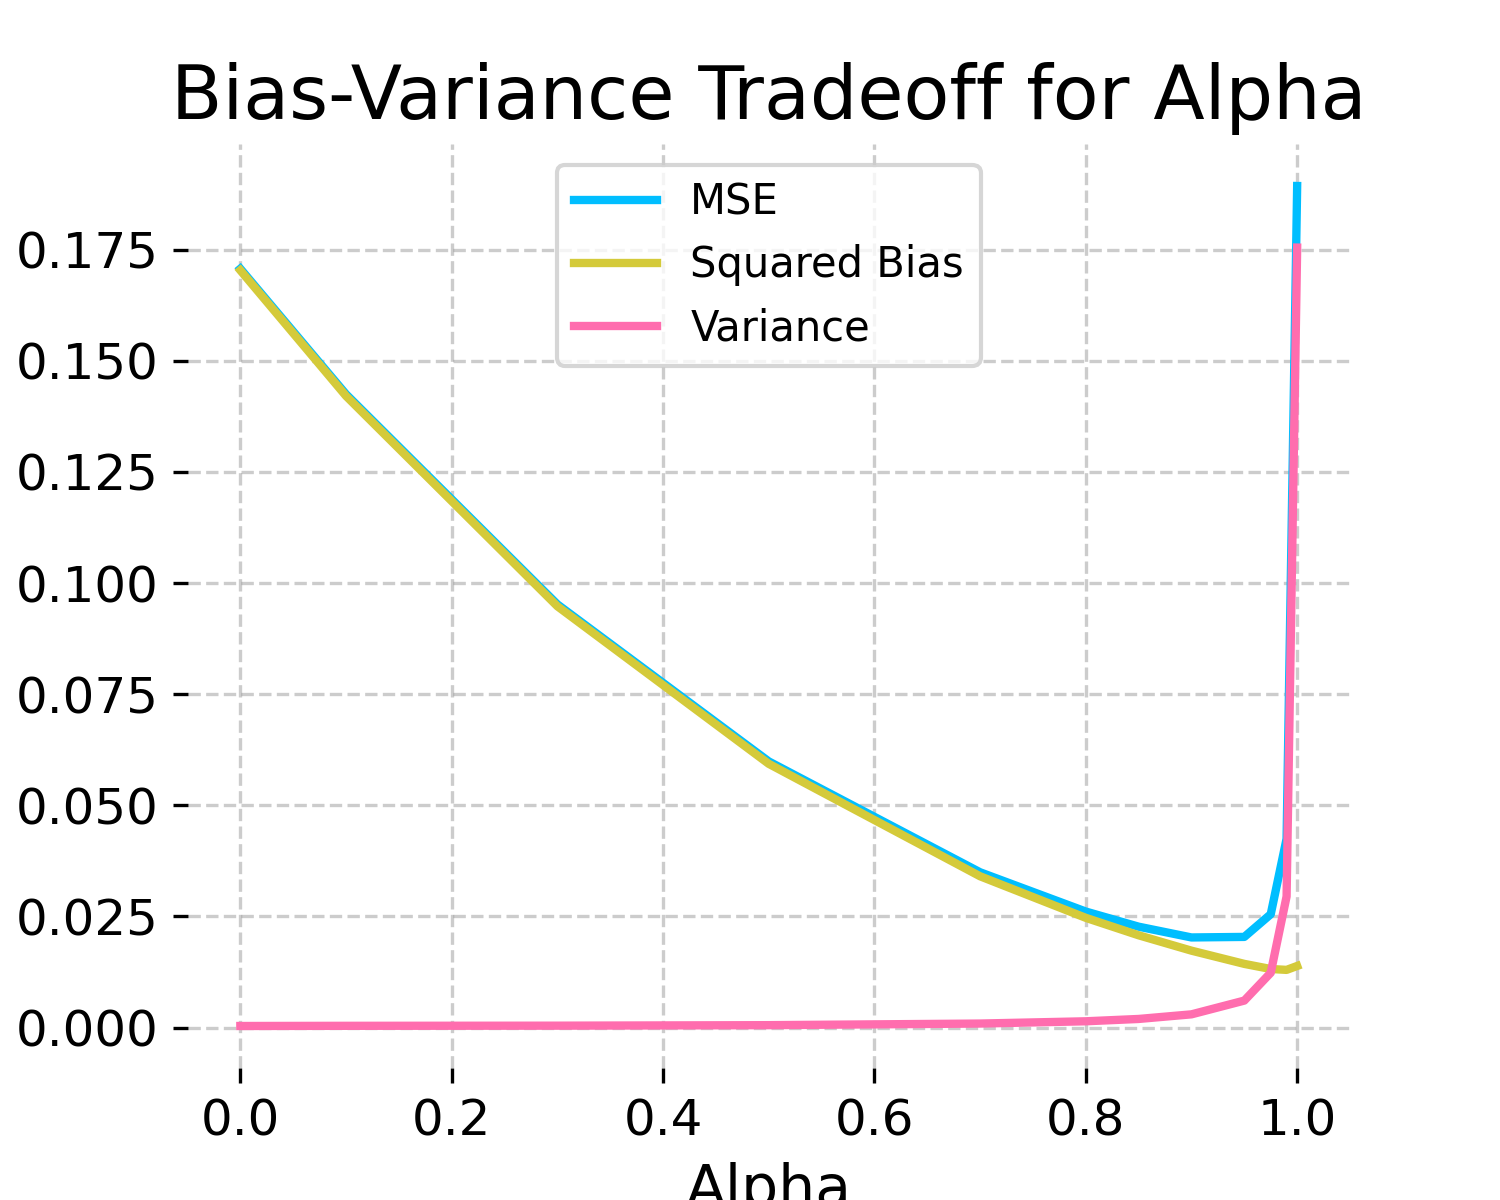
\includegraphics[width=\arxiv{10cm}{\textwidth/3}]{../imgs/095/biasvar.png}
    \caption{Illustration of the bias-variance tradeoff induced by the discounting hyperparameter $\alpha$, on the Dhaka cholera model of \cite{king08}. We display the MSE of score estimates for the trend in transmission, evaluated at the MLE.}
    \label{fig:biasvar}
\end{figure}

\subsection{Summary of Theoretical Guarantees}

The construction of MOP-$\alpha$ bypasses the issue of differentiating through a Monte Carlo algorithm with discontinuous resampling by turning it into a problem of differentiating through a simulator and a series of measurement density ratios.
We defer the theoretical analysis of MOP-$\alpha$ to Section \ref{sec:thms}, but first we highlight a few key results.
MOP-$\alpha$ estimates the likelihood and conditional distributions of latent variables, as one expects of a particle filter (Theorem \ref{thm:mop-targeting}).
When differentiated, we obtain the estimators of \cite{poyiadjis11, scibior21, naesseth18} as special cases (Theorem \ref{thm:mop-functional-forms}).
In particular, MOP-$1$ is consistent for the score (Theorem \ref{thm:mop-grad-consistency}), has rates for its bias and variance under different choices of $\alpha$ (Theorem \ref{thm:mop-biasvar}) that illustrate the desirable bias-variance tradeoff observed empirically in Figure \ref{fig:biasvar}, and enjoys a linear rate of convergence for gradient descent with the resulting gradient estimate (Theorem \ref{thm:mop-convergence}).  



\section{Practical Maximum-Likelihood Estimation}

%One can think of MOP-$\alpha$ as taking a likelihood estimate at $\phi$, reweighting it to instead target the likelihood at $\theta$, and then taking the derivative with respect to $\theta$ of the above estimate. 

If $\theta$ is evaluated at $\phi$, the particles at $\theta$ and $\phi$ coincide. One then only needs to run one particle filter at $\theta=\phi$, setting the particles at $\phi$ to be copies of the particles at $\theta$ where gradients don't propagate. This is done algorithmically through the \texttt{stop\_gradient()} function in \texttt{JAX}, providing a mathematical justification for the use of the stop-gradient operation by \cite{scibior21}.

\subsection{Optimization}

This still leaves us with the question of designing an effective procedure for likelihood maximization with MOP-$\alpha$. We propose a simple algorithm we call Iterated Filtering with Automatic Differentiation (IFAD) in Algorithm \ref{alg:ifad} that runs a few iterations of IF2 to warm-start an iterative (first or second-order) method that uses the MOP-$\alpha$ gradient estimate. This leverages IF2's quick empirical convergence to a neighborhood of the MLE, overcoming the tendency of gradient methods to get stuck in saddle points and local minima. Conversely, switching to gradient ascent with MOP-$\alpha$ score estimates lets one bypass the difficulty that IF2 has with optimizing the last few units of log-likelihood. Combining these two methods in this way lets us enjoy the best of both worlds.

The  convergence of IF2 (and so the first stage of IFAD) to a neighborhood of the MLE happens rapidly in practice. 
In the case of the Dhaka cholera model of \cite{king08}, when an aggressive geometric cooling multiplier of 0.95 and initial random walk standard deviation of 0.02 is used, initial convergence happens within 40 iterations. 
Finding the MLE itself with IF2, however, takes much longer, as one has to use a less aggressive cooling rate to do so. 
For example, \cite{ionides15} use 100 iterations with the Dhaka cholera model of \cite{king08}, while \cite{wheeler23} use 200 with Model 1 in \cite{lee20}. 
By simply requiring that the first stage of IFAD get to a neighborhood of the MLE and not the MLE itself, we are able to substantially reduce the number of IF2 iterations required. 

\subsection{Linear Convergence Rates}

On the other hand, the second stage of IFAD enjoys a linear convergence rate under the usual smoothness and strong convexity assumptions in the theory of convex optimization, as we show below in Theorem \ref{thm:mop-convergence}.

\begin{thm}[Linear Convergence of IFAD]
    
Consider the second stage of IFAD (Algorithm \ref{alg:ifad}) where one stops if $\|\nabla_\theta \hat\ell^\alpha(\theta_m)\| \leq (1+\sigma) \epsilon$, where $\sigma \geq \frac{4 \Gamma}{(1-\beta)}$, for some $\beta \in (0,1)$. Assume $-\ell$ is strongly convex and smooth, $\gamma I \preceq \nabla_\theta^2 (-\ell) \preceq \Gamma I$. Choose the learning rate $\eta$ such that $\eta \leq \frac{c(1-\beta)}{2\Gamma}$. Then, for sufficiently large $\alpha$ and $J$ to ensure the score estimate is an $\epsilon$-approximation and the minimum eigenvalue of $H$ is greater than some $c > 0$ for all $m$ with probability at least $1-\delta$, the second stage of IFAD converges linearly to the MLE:
\arxiv{}{\vspace*{-2mm}}
$$
\ell(\theta^*) - \ell(\theta_{m+1}) \leq \Big(1-\eta\beta\, \frac{8\gamma}{9c}\Big)\big(\ell(\theta^*)-\ell(\theta_m)\big).
$$
\label{thm:mop-convergence}
\end{thm}
\arxiv{}{\vspace*{-5mm}}
We borrow from tools in the field of randomized numerical linear algebra \cite{mahoney16} to solve this problem. The proof, which is similar to that of Theorem 6 in \cite{mahoney16}, is deferred to \arxiv{Appendix~\ref{appendix:convergence}}{the supplementary information}. For simplicity, we only prove this for MOP-$1$ and note that the general case follows as the required $\epsilon$-approximation can still be obtained for sufficiently large $\alpha$. When $\alpha=1$, the required $J$ is given in the supplementary information in Lemmas \ref{lemma:grad_bound} and \ref{lemma:hess_bound}. This result shows that particle estimates for the gradient can enjoy the same linear convergence rate on well-conditioned problems as gradient descent with access to the score. As , we note that it is possible.

We therefore see that the second stage of IFAD converges linearly to the MLE if (1) the log-likelihood surface is $\gamma$-strongly convex in a neighborhood of the MLE and (2) the first stage of IFAD successfully reaches a (high-probability) basin of attraction of the MLE. This happens fairly often in practice, for example, when sufficient regularity conditions for local asymptotic normality of the MLE hold. We conjecture that this applies to the entirety of IFAD, as IF2 converges very quickly to a neighborhood of the MLE, and will explore this in future work.

%IF2 posesses some SGD-like qualities, including what looks like linear convergence to a ball around the MLE with width determined by the random walk standard deviation. We will explore this conjecture in future work.

%While this theoretical guarantee currently only holds for IFAD-1, as it forms a particle approximation of the score as in \cite{poyiadjis11}, one can also extend this for a similar guarantee if the bias for the gradient estimate given by MOP-$\alpha$ for $\alpha < 1$ is small enough. For general $\alpha$, including MOP-0, the analysis then becomes more complicated, as one needs to handle the case of biased gradient descent. However, if future measurements $y_{n+1:N}^*$ do not provide a large amount of information on the identification of the current state $x_n$ given past and current measurements $y_{0:n}^*$, as mentioned in \cite{corenflos21}, the bias may be small enough for it to not present too much of a problem.

%The warm start allows gradient methods to shine, as regularity conditions ensure that the likelihood surface is well-behaved enough in this neighborhood that the aforementioned issues with saddle points and local minima are alleviated. 

\begin{algorithm}[H]
	\caption{IFAD}
    \label{alg:ifad}
	    \textbf{Input:} Number of particles $J$, timesteps $N$, IF2 cooling schedule $\eta_m$, MOP-$\alpha$ discounting parameter $\alpha$, $\theta_0$, $m=0.$\newline
        Run IF2 until initial "convergence" under cooling schedule $\eta_m$, or for a fixed number or iterations, to obtain $\{\Theta_j, j=1,...,J\}$, set $\theta_m := \frac{1}{J}\sum_{j=1}^J \Theta_j.$\newline
		\textbf{While} procedure not converged: \newline
		\hspace*{4mm} Run Algorithm \ref{alg:mop} to obtain $\hat\loglik(\theta_m).$ \newline
		\hspace*{4mm} Obtain $g(\theta_m) = \nabla_{\theta_m} \big(-\hat\loglik(\theta_m)\big)$, $H(\theta_m)$ s.t. $\lambda_{\min}\big(H(\theta_m)\big) \geq c$. \newline
		\hspace*{4mm} Update $\theta_{m+1} := \theta_m - \eta (H(\theta_m))^{-1} g(\theta_m)$, $m:=m+1.$ \newline
		\textbf{Return} $\hat{\theta} := \theta_m.$
\end{algorithm}


\section{Application to a Cholera Transmission Model}

The cholera transmission model that \cite{king08} developed for Dhaka, Bangladesh, has been used to benchmark the performance of various POMP inference methods \cite{ionides15, fasiolo16, wycoff24}, and we employ it here for the same purpose.
This model categorizes individuals in a population as susceptible, $S(t)$, infected, $I(t)$, and recovered, $R(t)$ and so is called an SIR compartmental model.
In this case, the compartment $R(t)$ is further subdivided into 
%. where the population at time $t$, $H_t$, is divided into the susceptible compartment $S_t$, infected compartment $I_t$, and
three recovered compartments $R^1(t)$, $R^2(t)$, $R^3(t)$ denoting varying degrees of cholera immunity.
We write $P(t)$ for the total population, and $M_n$ for the cholera deaths in each month.
As in \cite{king08, ionides15}, the transition dynamics follow a series of stochastic differential equations:
\vspace*{-1mm}
\begin{align*}
    dS&=\big(k \epsilon R^k+\delta(S-P)-\lambda(t) S\big)\, dt+d P-({\sigma S I}/{H})\, dB, \\
    dI&=\big(\lambda(t) S-(m+\delta+\gamma) I\big)\, dt+({\sigma S I}/{H})\, dB, \\
    dR^1&=\big(\gamma I-(k \epsilon+\delta) R^1\big)\, dt, \hspace{2mm} \dots \\
    dR^k&=\big(k \epsilon R^{k-1} -(k \epsilon+\delta) R^k\big)\, dt,
    \vspace*{-2mm}
\end{align*}
with Brownian motion $B(t)$, cholera death rate $m$, recovery rate $\gamma$, mean immunity duration $1/\epsilon$, standard deviation of the force of infection $\sigma$, and population death rate $\delta=0.02$. The force of infection, $\lambda_t$, is modeled by splines $(s_j)_{j=1}^6$
\vspace*{-2mm}
\begin{equation*}    \lambda_t=\exp\hspace{-1mm}\left(\hspace{-.5mm}\beta_{\text{trend}}(t-t_0)+\hspace{-1mm}\sum_{j=1}^{6} \beta_j s_j(t)\hspace{-1mm}\right)\hspace{-1mm}\frac{I}{P} + \exp\hspace{-1mm} \left(\sum_{j=1}^{6} \omega_j s_j(t)\hspace{-1mm}\right)\hspace{-1mm},
    \vspace*{-2mm}
\end{equation*}
where the coefficients $(\beta_j)_{j=1}^6$ model seasonality in the force of infection, $\beta_{\text{trend}}$ models the trend in the force of infection, and the $\omega_j$ represent seasonality of a non-human environmental reservoir of disease.
The measurement model for observed monthly cholera deaths is given by 
    $Y_n \sim \gN(M_n, \tau^2M_n^2)$,
where $M_n=\gamma\int_{t_{n-1}}^{t_n}I(s)\, ds$ is the modeled number of cholera deaths in that month.


\begin{figure}
    \centering
    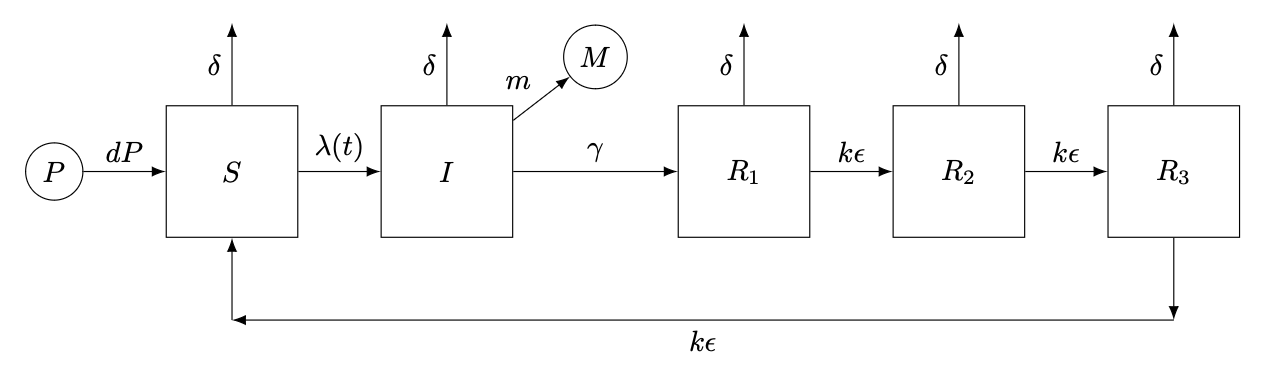
\includegraphics[width=\arxiv{14cm}{\textwidth/2}]{../imgs/095/tikzcholera.png}
    \vspace*{-7mm}
    \caption{A compartment flow diagram for the Dhaka cholera model from \cite{king08}.}
    \label{fig:tikz-cholera}
\end{figure}

\subsection{Results}

We tested IFAD against IF2 on a global search problem for the Dhaka cholera model.
We re-implemented IF2 to do so, but we compare our results with the results of \cite{ionides15} (labeled "IF2 2015").
Our re-implementation ourperforms that of \cite{ionides15}, likely due to a better choice of algorithmic parameters.
For each method, we performed 100 searches, initialized with 100 initial starting parameter vectors drawn uniformly from the same wide bounding box used in \cite{ionides15}. We summarize our findings below. 

% \kevin{Dynamically save to a tex file and load from there}
  
\begin{table}[h!]
\centering
\begin{tabular}{lrr}
\toprule
 & Best Log-Likelihood & Rank \\
\midrule
IFAD-0.97 & -3750.2 & 1 \\
IFAD-0 & -3752.2 & 2 \\
IFAD-1 & -3754.6 & 3 \\
IF2 & -3758.2 & 4 \\
IF2 2015 & -3768.6 & 5 \\
\bottomrule
\end{tabular}

\caption{Maximum log-likelihood found by IF2, IFAD, and MOP alone. IFAD performs the best among all methods. Our implementation of IF2 outperforms that of \cite{ionides15}, but still ultimately underperforms IFAD. IFAD manages to find the MLE, matching the highest log-likelihood previously found in the Dhaka cholera model implemented within the \texttt{pomp} package of \cite{king16}.}
\label{table:mle}
\end{table}

\paragraph{IFAD Successfully Finds the MLE:} Previously, an MLE at a log-likelihood of $-3748.6$ was reported by \cite{king16}.
This MLE was obtained with much computational effort, using many global and local IF2 searches, and with the assistance of likelihood profiling.
Meanwhile, \cite{ionides15} only achieve a maximum log-likelihood of $-3768.6$, while the best log-likelihood found by \cite{king08} was only $-3793.4$.
Despite being initialized for a global search, IFAD manages to get much closer to the MLE over the $100$ searches than \cite{ionides15} and finds it up to $2.5$ standard deviations of Monte Carlo error, as seen in Table~\ref{table:mle}.
On this problem, the sequence of local searches, refinement, and likelihood profiling that was previously required for finding the MLE is not necessary with the IFAD algorithm. 
In other words, the improvement in numerical efficiency of IFAD over IF2 is so large that routine application of IFAD (consisting of a collection of Monte Carlo replications from random starting points) generates results outside the reach of a routine application of IF2. 
When interpreting Table~\ref{table:mle}, bear in mind that by Wilks' Theorem, any difference of over $1.92$ log units has statistical relevance when testing one parameter at the $0.05$ significance level, and therefore potentially has scientific value.

\paragraph{IFAD Outperforms Both IF2 and MOP Alone:} While IF2 quickly approaches a neighborhood of the MLE within only 40 iterations, performing IF2 alone ultimately fails to achieve the last few log-likelihood units, as no IF2 search comes within 7 log-likelihood units of the MLE (as seen in Figure \ref{fig:scatter}). Conversely, when we tried gradient descent with MOP alone, we encountered many failed searches. This is a difficult, nonconvex, and noisy problem with $18$ parameters, and the search gets stuck in local minima and saddle points, failing to approach the MLE. 

IFAD, in comparison, approaches the MLE quickly due to the IF2 warm-start (as seen in Figure \ref{fig:optim}) and also succeeds at refining the coarse solution found by the warm-start with MOP gradient steps to find the MLE (as seen in Figures~\ref{fig:scatter} and \ref{fig:boxplot}). IFAD therefore successfully combines the best qualities of IFAD and MOP, outperforming either of them alone.
Monte~Carlo replication is appropriate for IFAD, or any Monte Carlo algorithm used to solve a challenging numerical problem, but Figure~\ref{fig:boxplot} shows that IFAD can find higher likelihood values, more quickly and more reliably than the previous state-of-the-art. 
In particular, Figure~\ref{fig:boxplot} shows that IFAD with $\alpha=0.97$ can maximize the challenging likelihood of \cite{king08} using a modest number of iterations and Monte Carlo replications, whereas previously it was necessary to carry out an extensive customized search or to live with an incompletely maximized likelihood.

For the results presented here, we did not include the many common heuristics used in the machine learning and optimization literature in the gradient descent stage.
We used constant learning rates of $0.01, 0.05$, and $0.2$ for IFAD-$1,0,$ and $0.97$ respectively, and a constant cooling rate of $0.95$ for our IF2 implementation.
While techniques such as annealing learning rates, gradient normalization, and momentum could further improve the performance of IFAD in other simulations we performed, we chose to report the results of the simplest implementation to serve as a baseline for the method's performance.
The results for this basic implementation are already sufficient to show the high potential of the approach.

\begin{figure}[htbp!]
    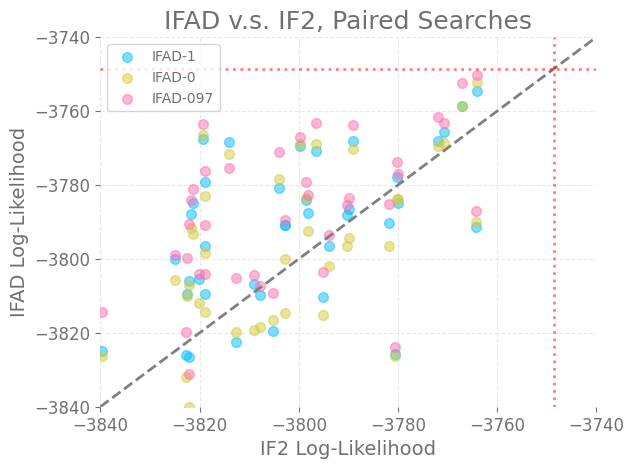
\includegraphics[width=\arxiv{8cm}{\textwidth/\real{4.2}}]{../imgs/095/pairs.png}
    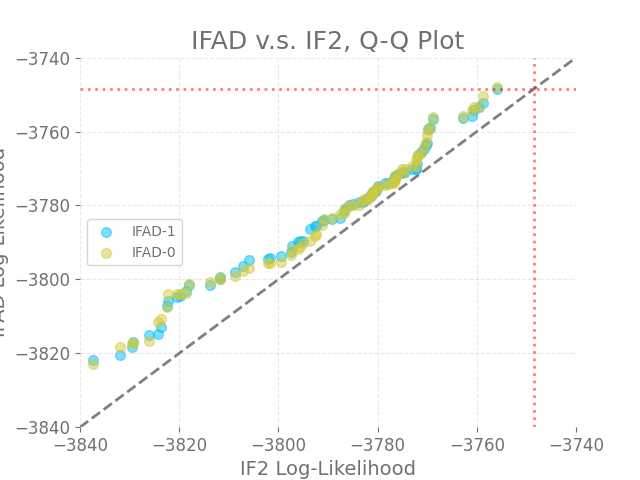
\includegraphics[width=\arxiv{8cm}{\textwidth/\real{4.2}}]{../imgs/095/qq.png}
    \caption{Scatterplots depicting the performance of IFAD against that of IF2. \textbf{Left:} Paired searches from the same starting point. Controlling for initial starting point, tuning $\alpha$ allows IFAD-$0.97$ to strictly improve on IF2, \cite{poyiadjis11}, and \cite{naesseth18}, on almost every iteration. \textbf{Right:} Q-Q plot of ranked IFAD searches against ranked IF2 searches. It is clear that on average, IFAD performs best, and manages to find the MLE while no IF2 search successfully gets within 7 log-likelihood units of it. The dotted red line shows the true maximized log-likelihood. }
    \label{fig:scatter}
\end{figure}

%\kevin{Include plots of IFAD vs Poyiadjis and Naesseth only in the supplemental information}

%% \ed{Labeling A and B would be more conventional than Left and Right, and also easier to refer to in the text.}
  
\begin{figure}[ht]
    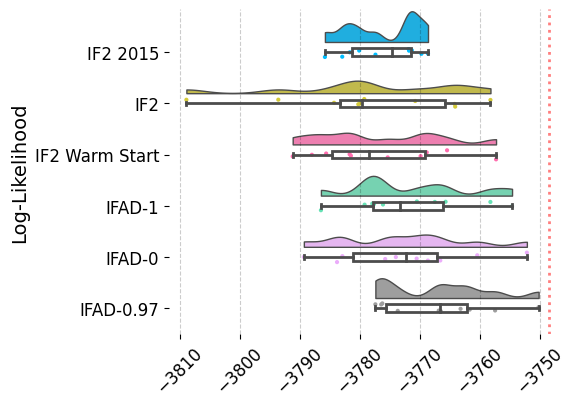
\includegraphics[width=\arxiv{8cm}{\textwidth/\real{4.2}}]{../imgs/095/boxplot.png}
    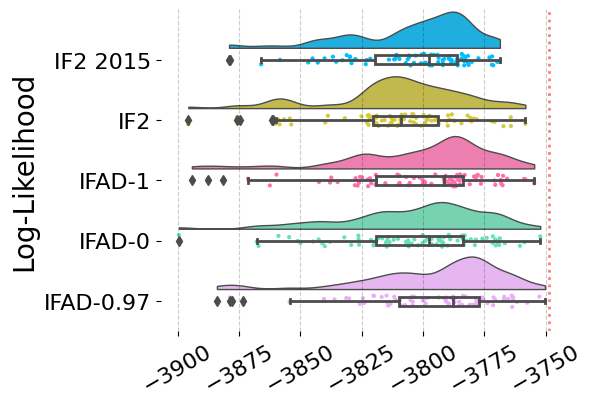
\includegraphics[width=\arxiv{8cm}{\textwidth/\real{4.2}}]{../imgs/095/boxplot_all.png}
    \caption{\textbf{Left:} Raincloud plot depicting the performance of IFAD and IF2 where we plot the results of the best run out of every ten runs, representing the common procedure of running a few searches and choosing the best one. \textbf{Right:} Raincloud plot of all searches. IFAD outperforms all other methods, and the gradient steps improve on the warm-start given by running 40 IF2 iterations.
    The dotted red line shows the true maximized log-likelihood.}
    \label{fig:boxplot}
\end{figure}

\begin{figure}[ht]
    \centering
    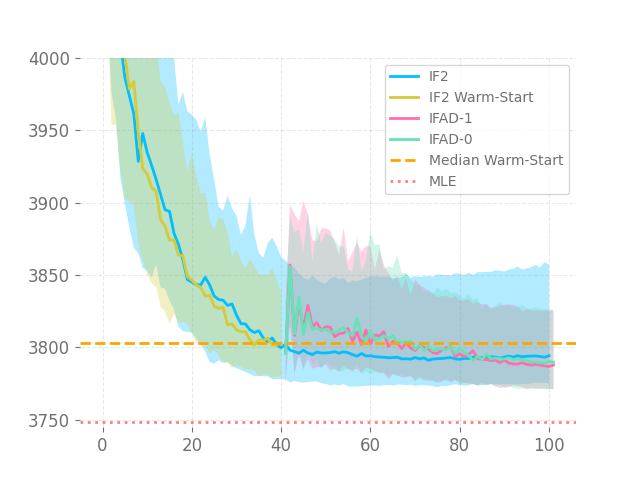
\includegraphics[width=\arxiv{10cm}{\textwidth/3}]{../imgs/095/optim.png}
    \caption{Optimization progress of IFAD and IF2. The dashed orange line depicts the median warm-start given by running 40 IF2 iterations. While running 60 more iterations of IF2 improves upon the median warm-start, doing so ultimately underperforms IFAD. We see that IFAD has better tail control and successfully reaches the MLE. 
    We use a dotted red line to display the MLE.}
    \label{fig:optim}
\end{figure}

\section{Application to Bayesian Inference}
\label{sec:bayes}

Particle MCMC, as introduced by \cite{andrieu10}, is arguably the most popular method for full-information plug-and-play Bayesian inference for POMP models.
The plug-and-play property enables its use in simulation-based Bayesian inference for complex scientific models where computing transition densities is not feasible, such as in disease modeling.
However, the particle Metropolis-Hastings algorithm often experiences slow mixing and requires long burn-in periods.
For instance, \cite{fasiolo16} reported needing $700,000$ burn-in iterations for effective sampling in a cholera model.
This computational burden necessitated simplifying the scientific model to reduce computational costs, by adjusting the length of each Euler timestep to be a month instead of a day. 

We employ a NUTS sampler powered by a MOP-$\alpha$, with a nonparametric empirical prior initialized by the IF2 warm start from the previous section.
To construct the prior, we perform a kernel density estimate (KDE) on the parameter swarm from the warm start, and use the output of that as an empirical prior.
The KDE is performed to ensure some degree of mutual contiguity between the densities.
This yields a prior that is roughly equivalent to a parameter cloud centered at some point in the neighborhood of the MLE, with a standard deviation of $\sqrt{(0.02\cdot0.95^{40})^2 \cdot 600}\approx 6.3\%$ of the MLE.
Using a NUTS sampler powered by MOP-$\alpha$ with this prior significantly lowers the mixing time of the Markov chain to as little as $500$ iterations, as seen in Figure \ref{fig:nuts-eb}. 

\begin{figure}[t!]
    \centering
    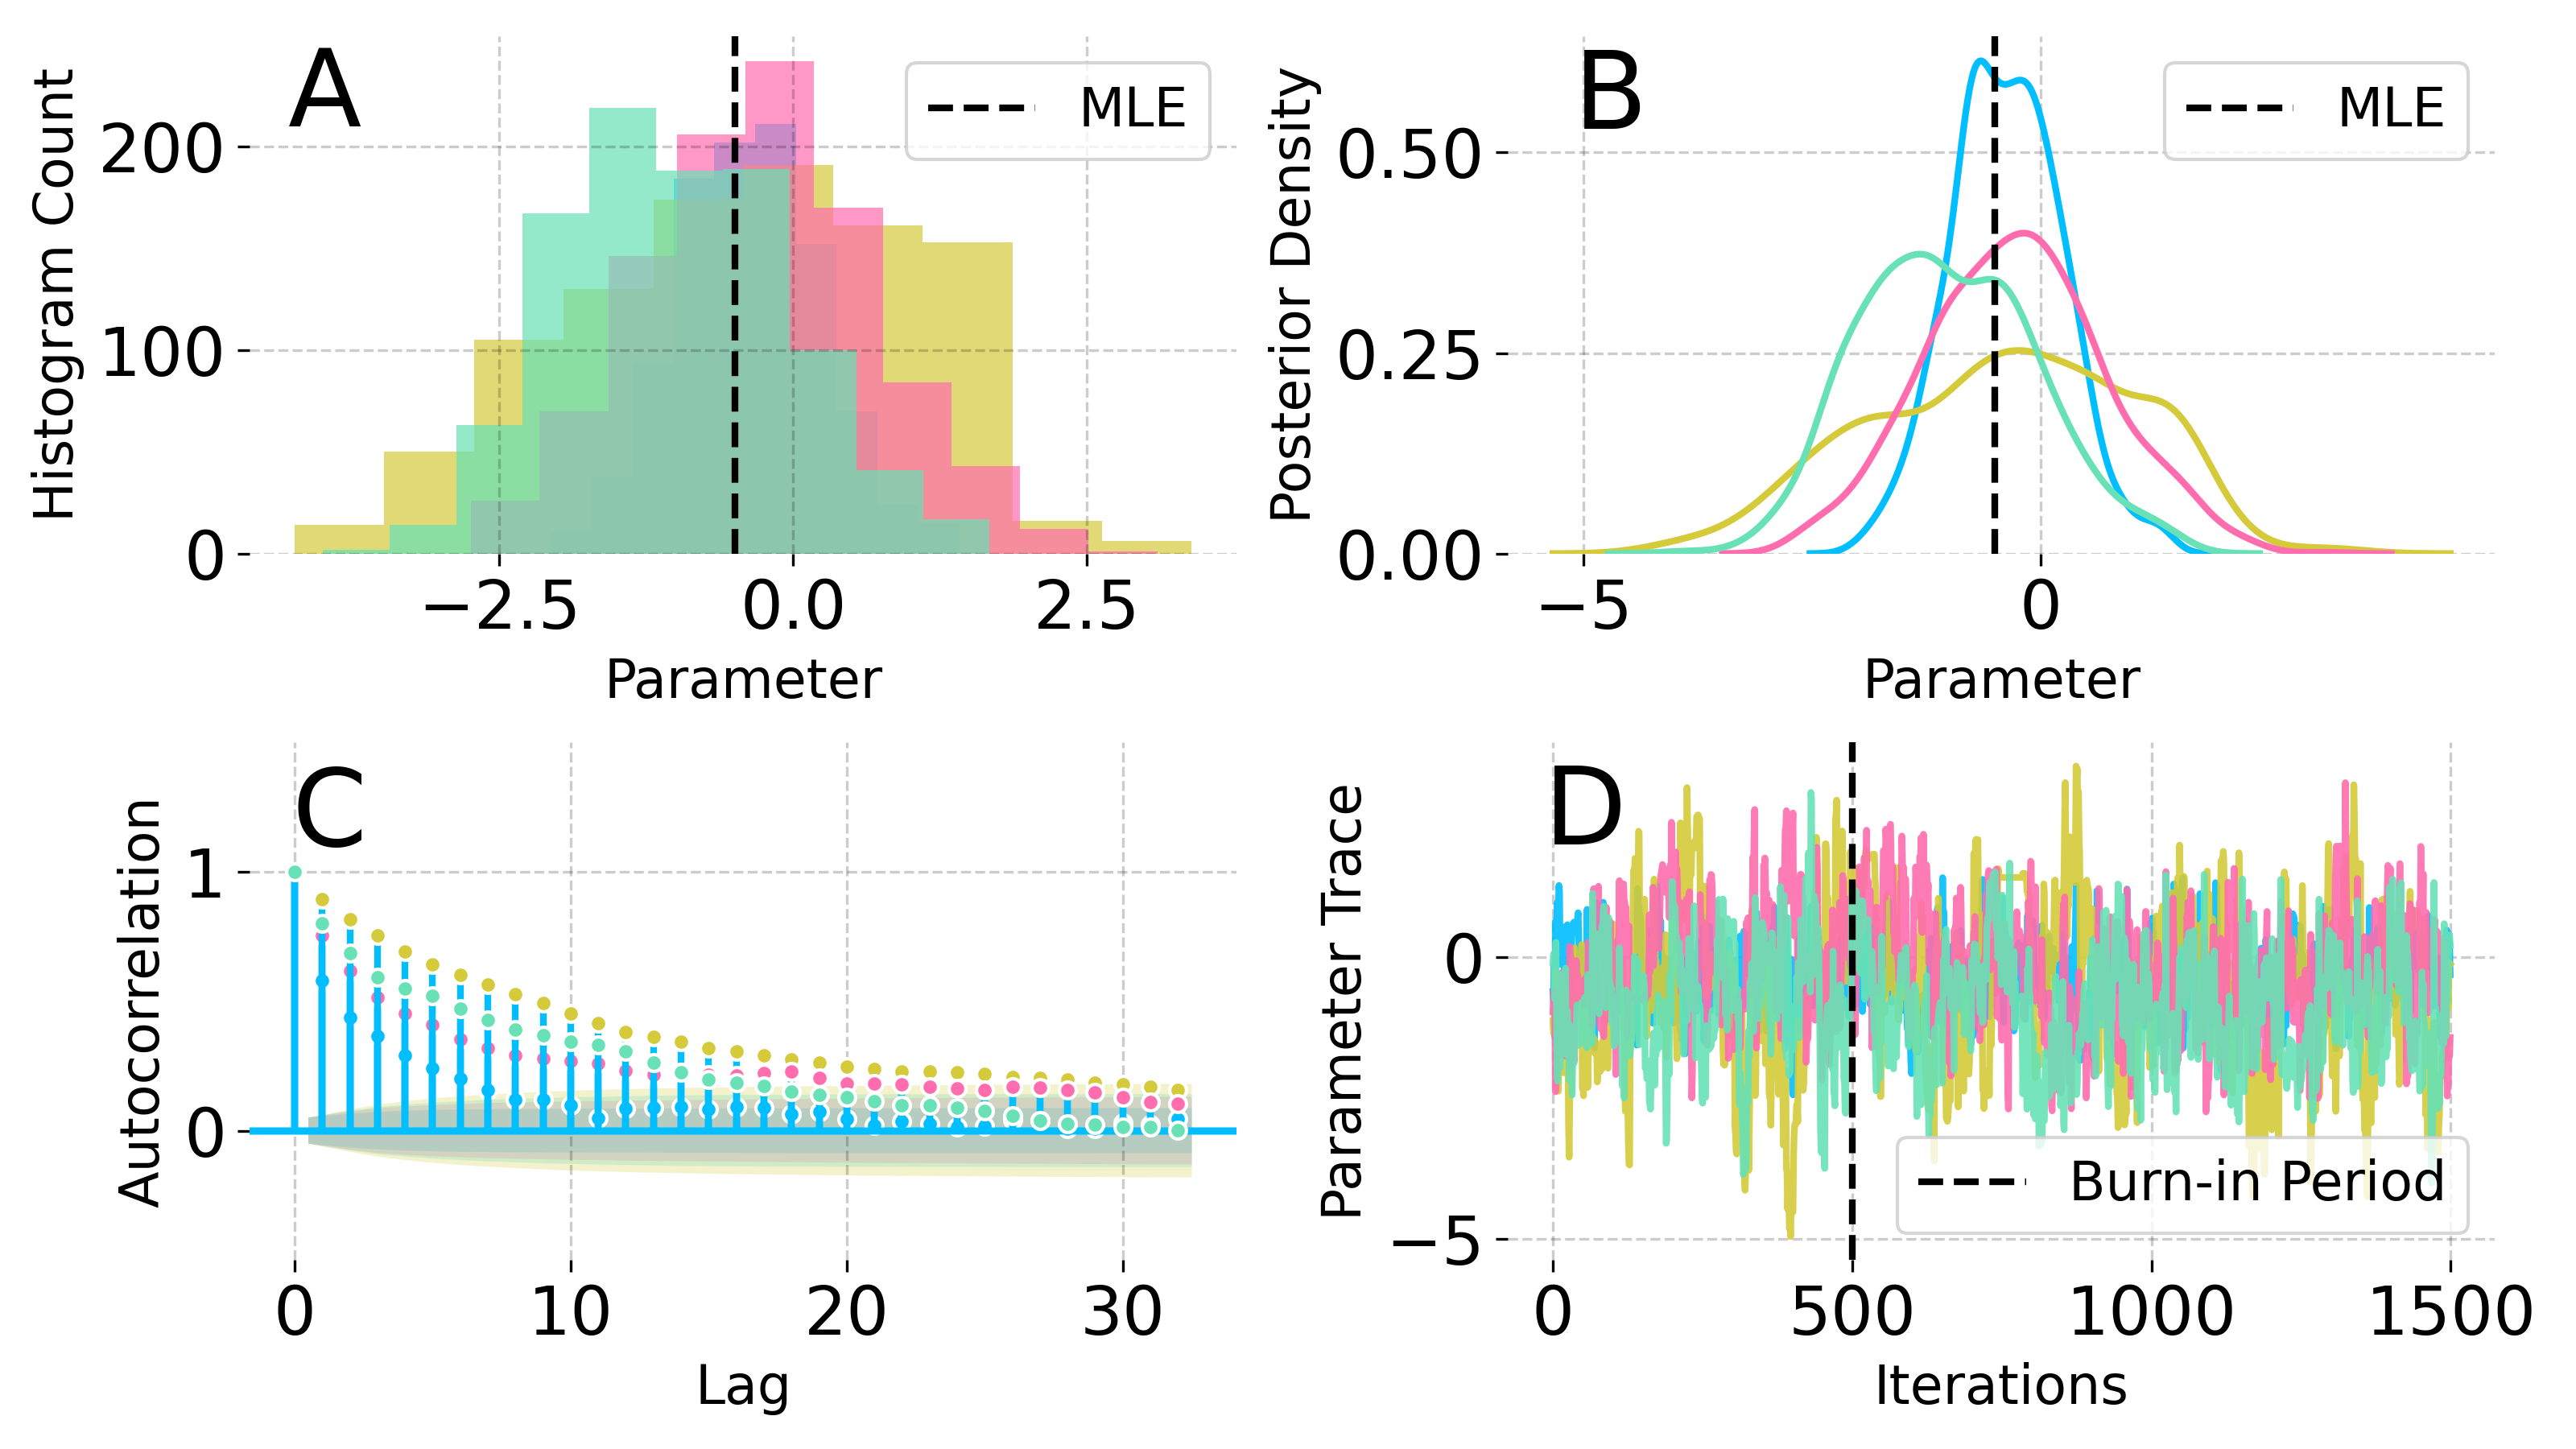
\includegraphics[width=\textwidth/\real{1.25}]{../imgs/pmcmc/nuts_eb.png}
    \caption{Convergence diagnostics for NUTS with the informative nonparametric empirical Bayes prior from applying KDE to preliminary searches using IF2, with $4$ chains. We display the results for the trend parameter in the Dhaka cholera model of \cite{king08}. The NUTS sampler mixes quickly, and the posterior estimates from each chain share roughly the same posterior mode.}
    \label{fig:nuts-eb}
\end{figure}

For completeness, we note that without the empirical Bayes-style prior from IF2, NUTS with the MOP-$\alpha$ estimate alone tended to diverge.
In contrast, particle Metropolis-Hastings (with or without the empirical Bayes prior from IF2) fails to effectively explore the parameter space.
We display the results of the above in Figures \ref{fig:mh} and \ref{fig:nuts} \arxiv{in Appendix~\ref{appendix:bayes}}{within the supplementary information}. 
The result obtained in this section, of a speedup in the mixing time of particle MCMC by over three orders of magnitude, provides hope that particle Bayesian inference might finally be practical for the complex scientific models commonly encountered in areas like epidemiology.

\section{Theoretical Analysis of MOP-$\alpha$}
\label{sec:thms}

Here, we will show that MOP-$\alpha$ targets the filtering distribution and likelihood under $\theta$, is consistent when $\alpha=1$, and characterize rates for its bias and variance under different choices of $\alpha$. To do so, we require the following assumptions:

\begin{enumerate}[label=(A\arabic*),itemsep=-1.2ex] 
    \item \textbf{Continuity of the Likelihood.} $\ell(\theta)$ has more than two continuous derivatives in a neighborhood $\left\{\theta: \ell(\theta)>\lambda_1\right\}$ for some $\lambda_1<\sup _{\varphi} \ell(\varphi)$. \label{assump:conti-lik}
    \item \textbf{Bounded Process Model.} There exist $\underbar{M}, \bar{M}$ such that $0 < \underbar{M} \leq f_{X_n|X_{n-1}}(x_n | x_{n-1};\theta) \leq \bar{M} < \infty$. \label{assump:bounded-process}
    \item \textbf{Bounded Measurement Model.} There exist $\underbar{G}, \bar{G}$ such that $0<\underbar{G} \leq f_{Y_n \mid X_n}\left(y_n^* \mid x_n; \theta\right) \leq \bar{G}<\infty$ and there exists $G'(\theta)$ with $\|\nabla_\theta \log f_{Y_n \mid X_n}\left(y_n^* \mid x_n; \theta\right)\|_\infty \leq G'(\theta)< \infty$. \label{assump:bounded-measurement}
    \item \textbf{Bounded Gradient Estimates.} There are functions $G(\theta), H(\theta): \Theta \to [0,\infty)$ uniformly bounded by $G^*, H^*<\infty$, so the MOP-$\alpha$ gradient and Hessian estimates at $\theta=\phi$ are almost surely bounded by $G(\theta)$ and $H(\theta)$ for all $\alpha$. \label{assump:local-bounded-derivative}
    \item \textbf{Differentiability of Density Ratios and Simulator.} The measurement density, \arxiv{\\}{}$f_{Y_n|X_n}(y_n^*|x_n; \theta)$, and simulator have more than two continuous derivatives in $\theta$. \label{assump:diff-meas-and-sim}
\end{enumerate}

The fact that the likelihood estimate yielded by MOP-$\alpha$ has more than two continuous derivatives in $\theta$ follows from the construction of the likelihood estimate in equations \ref{eq:mop-conditional-likelihood} and \ref{eq:weighting-scheme}, as well as Assumptions \ref{assump:bounded-measurement} and \ref{assump:diff-meas-and-sim}. 

\subsection{MOP-$\alpha$ Targets the Filtering Distribution}


We show here that MOP-$\alpha$ targets the filtering distribution under $\theta$ and is strongly consistent for the likelihood under $\theta$ when $\alpha=1$ or $\theta=\phi$.
Employing $\alpha<1$ lead to inconsistency when $\theta$ deviates from $\phi$, but this bias disappears as $\theta$ approaches $\phi$.

While the result is presented here as specific to MOP-$\alpha$, we actually prove a more general result in \arxiv{Appendix~\ref{appendix:targeting}}{the supplementary material}.
That is, we show a strong law of large numbers for triangular arrays of particles with off-parameter resampling, where we resample the particles according to an arbitrary resampling rule not necessarily in proportion to the targeted distribution of interest and employ weights that encode the cumulative discrepancy between the resampling and the target distribution instead of equal weights.

%\kevin{Should we just show the general result? That is, for an arbitrary set of indices $k_{n,j}$ generated in proportion to some arbitrary weights $\pi_{n,j}$ that do not necessarily sum to $1$ as the estimate is self-normalized, reweighting the particles by $w_{n,a(j)}g_{n,a(j)}/\pi_{n,a(j)}$ targets the posterior. $\pi_{n,j}$ can depend on $\{(x_{n,1:J},g_{n,1:J})\}$ as long as the resampling is carried out independently of $\{(x_{n,1:J},g_{n,1:J})\}$, conditional on $\pi_{n,1:J}$}

\begin{thm}[MOP-$\alpha$ Targets the Filtering Distribution and Likelihood]
    \label{thm:mop-targeting}
    When $\alpha=1$ or $\theta=\phi$, MOP-$\alpha$ targets the filtering distribution under $\theta$ and is strongly consistent for the likelihood under $\theta$. That is, for $\pi_n(\theta)=f_{X_{n}|Y_{1:n}}(x_n|y_{1:n}^* ; \theta)$ and any measurable and bounded functional $h$ and for $\hat\lik(\theta) = \prod_{n=1}^N L_n^{A,\theta,\alpha}$ or $\prod_{n=1}^N L_n^{B,\theta,\alpha}$, it holds that
    \arxiv{}{\vspace*{-2.5mm}}
    \begin{equation} \nonumber
        \frac{\sum_{j=1}^J h(x_{n,j}^{F, \theta}) \, w_{n,j}^{F,\theta}}{\sum_{j=1}^J w_{n,j}^{F,\theta}} \stackrel{a.s.}{\to} E_{\pi_n(\theta)} \big[h(X_n)\big], \hspace{5mm} \hat\lik(\theta)  \stackrel{a.s.}{\to} \lik(\theta).
    \arxiv{}{\vspace*{-2.5mm}}
    \end{equation}
\end{thm}

%\kevin{Write the supplement formally with Del Moral-lite language, going into full detail with the proofs and calculations.}

\begin{proof}
    We provide a proof sketch here, deferring most of the details, and discussion of the after-resampling conditional likelihood estimate $L_n^{A,\theta,\alpha}$, to \arxiv{Appendix~\ref{appendix:targeting}}{the supplementary information}. 
    When $\theta=\phi$, regardless of the value of $\alpha$, the ratio ${g_{n,j}^\theta}/{g_{n,j}^\phi}=1,$ and this reduces to the vanilla particle filter.
    When $\alpha=1$ and $\theta\neq\phi,$ suppose inductively that $\{(X^{F,\theta}_{n-1,j},w^{F,\theta}_{n-1,j})\}_{j=1}^J$ targets $f_{X_{n-1}|Y_{1:n-1}}(x_{n-1}|y^*_{1:n-1};\theta)$.
    It can then be shown that $\{(X^{P,\theta}_{n,j},w^{P,\theta}_{n,j})\}_{j=1}^J$ targets $f_{X_{n}|Y_{1:n-1}}(x_{n}|y^*_{1:n-1};\theta)$, that $\{(X^{P,\theta}_{n,j},w^{P,\theta}_{n,j} \, g^\theta_{n,j} )\}_{j=1}^J$ targets  $f_{X_{n}|Y_{1:n}}(x_{n}|y^*_{1:n};\theta)$, and that weighting the particles by $(X^{F,\theta}_{n,j},w^{F,\theta}_{n,j}) = (X^{P,\theta}_{n,k_j}, w^{P,\theta}_{n,k_j} \, g^\theta_{n,k_j} \big/ g^\phi_{n,k_j})$,
    resampling the $k_j$ with probabilities proportional to $g^\phi_{n,j}$, also targets $f_{X_{n}|Y_{1:n}}(x_{n}|y^*_{1:n};\theta)$.
    If the likelihood is estimated with the before-resampling conditional likelihoods $\hat\lik(\theta) = \prod_{n=1}^N L_n^{B,\theta,\alpha}$, the strong consistency is a direct consequence of our earlier result that $\{ \big(X^{P,\theta}_{n,j},w^{P,\theta}_{n,j}\big) \}$ targets $f_{X_{n}|Y_{1:n-1}}(x_{n}|y^*_{1:n-1};\theta)$. 
\end{proof}




\subsection{MOP-$1$ Is Consistent for the Score}

Despite showing that the MOP-$1$ gradient estimate yields the estimate of \cite{poyiadjis11, scibior21} when applied to the bootstrap filter, \cite{poyiadjis11, scibior21} estimate the Fisher score by 
$$\frac{1}{J}\sum_{j=1}^J \nabla_\theta \log f_{X_{0:N}, Y_{1:N}}\left(x_{0:n,j}^{A, F,\theta}, y_{1:N}^* ; \theta\right)$$ and not
$$\frac{1}{J}\sum_{j=1}^J \nabla_\theta \log f_{Y_{1:N}| X_{1:N}}\left(y_{1:N}^* | x_{1:n,j}^{A, F,\theta}; \theta\right).$$
It is therefore not immediately apparent that these two converge to the same thing. As such we directly show the consistency of the MOP-$1$ gradient estimate below. 
We present an abbreviated proof here, postponing the full argument to \arxiv{Appendix~\ref{appendix:consistency}}{the supplement}.

\begin{thm}[Consistency of MOP-$1$ Gradient Estimate]
    The gradient estimate of MOP-$\alpha$ when $\alpha=1$, $\theta=\phi$ is strongly consistent for the score: $\nabla_\theta \hat\ell_J^1(\theta) \stackrel{a.s.}{\to} \nabla_\theta \ell(\theta)$ as $J \to \infty$.
    \label{thm:mop-grad-consistency}
\end{thm}
\begin{proof}
    Fix $\omega \in \Omega$, and set $\phi = \theta$, where $\theta$ is the point at which we wish to evaluate the gradient. The sequence $(\nabla_\theta \hat\lik_J^1(\theta)(\omega))_{J \in \mathbb{N}}$ is uniformly bounded over all $J$ by Assumption \ref{assump:local-bounded-derivative}. Again by Assumption \ref{assump:local-bounded-derivative}, the second derivative of $\hat\lik_J^1(\theta)(\omega)|_{\theta=\theta'}$ is also uniformly bounded over all $J$ by $H^*$ for almost every $\omega\in \Omega$ and every $\theta'\in \Theta$. So $(\nabla_\theta \hat\lik_J^1(\theta)( \omega))_{J \in \mathbb{N}}$ is uniformly Lipschitz, and therefore uniformly equicontinuous for almost every $\omega \in \Omega$.

    By Arzela-Ascoli, there is a uniformly convergent subsequence. But there is only one subsequential limit, as we can treat the gradient estimate at $\theta$ as a bounded functional of the particles by Assumption \ref{assump:local-bounded-derivative}, allowing us to apply Theorem \ref{thm:mop-targeting} to see that the sequence $(\nabla_\theta \hat\lik_J^1(\theta)(\omega))_{J \in \mathbb{N}}$ converges pointwise for $\theta=\phi$ and almost every $\omega \in \Omega$. So the whole sequence must converge uniformly to $\lim_{J \to \infty} \nabla_\theta \hat\lik_J^1(\theta)(\omega).$ 
    
    With uniform convergence for the derivatives established, we can swap the limit and derivative and obtain, in conjunction with the strong consistency $\hat{\lik}_J^1(\theta)(\omega) \stackrel{a.s.}{\to} \lik(\theta)$ in Theorem \ref{thm:mop-targeting}, that for almost every $\omega \in \Omega$, 
    $\lim_{J \to \infty} \nabla_\theta \hat\lik_J^1(\theta)(\omega) = \nabla_\theta \lim_{J \to \infty} \hat\lik_J^1(\theta)(\omega) = \nabla_\theta \lik(\theta).$
    The result then follows by the continuous mapping theorem. 
\end{proof}


\subsection{MOP-$\alpha$ Error, Bias and Variance}

We now provide a result showing that MOP-$\alpha$ has a desirable bias-variance tradeoff when $0<\alpha<1$.
This is achieved because it combines favorable properties from the low-variance but asymptotically biased estimate of \cite{naesseth18} and the high-variance but consistent estimate of \cite{poyiadjis11}. 
As the bias itself is difficult to analyze, we instead analyze the MSE and variance. 
The below result applies for any $\alpha \in [0,1)$, but not $\alpha=1$, as the gradient estimate when $\alpha=1$ has no forgetting properties. 

\begin{thm}
    \label{thm:mop-biasvar}
    When $\alpha\in (0,1)$ and $\theta=\phi$, define $\psi(\alpha)=(\alpha^k  + \alpha^{k+1} - \alpha)/(1-\alpha)$. 
    There exists an $\epsilon>0$ depending on $\bar{M}, \underbar{M}, \bar{G}, \underbar{G}$ as in \cite{karjalainen23} such that the MSE and variance of MOP-$\alpha$ are:
    \vspace*{-1ex}
    \begin{eqnarray}
        \E\big\|\nabla_\theta\ell(\theta) - \nabla_\theta \hat\ell^\alpha(\theta)\big\|_2^2 
        &\lesssim& \min_{k \leq N} Np \, G'(\theta)^2\left(k^2J^{-1}+(1-\epsilon)^{\floor{k/(c\log(J))}}+k+\psi(\alpha)\right), \label{eq:mop-mse}
        \\
        \Var\big(\nabla_\theta \hat\ell^{\alpha}(\theta)\big) &\lesssim& \min_{k\leq N} Np \, G'(\theta)^2\left(\frac{k^2}{(1-\alpha)^2J} + \frac{\alpha^{k}}{1-\alpha}N\right). \label{eq:mop-variance}
        \end{eqnarray}
\end{thm}
We defer the proof to \arxiv{Appendix~\ref{appendix:biasvar}}{the supplementary material}, but provide a brief outline here. 
The variance bound can be reduced to the approximation error between MOP-$\alpha$ and a variant called MOP-$(\alpha,k)$ where the discounted weights are truncated at lag $k$. 
The discount factor, $\alpha$, ensures strong mixing.
The covariance of the derivative of MOP-$(\alpha,k)$ can be controlled with Davydov's inequality and a standard $L^p$ error bound for the particle filter. 
The MSE bound considers the error between the score and MOP-$(1,k)$, and the error between MOP-$(1,k)$ and MOP-$\alpha$. 
The latter can be shown to be $\tilde{O}\big(Np \, G'(\theta)^2(k+\psi(\alpha))\big)$, and the former can be controlled with a result on the the forgetting of the particle filter from \cite{karjalainen23} and the very same $L^p$ error bound mentioned above. 

\paragraph{Interpretation:} Theorem \ref{thm:mop-biasvar} provides theoretical understanding of the results observed in Figure \ref{fig:biasvar} that show the empirically favorable bias-variance tradeoff enjoyed by MOP-$\alpha$.
The first term in the MSE bound in Equation \ref{eq:mop-mse} corresponds to the error of the particle approximation, the second mixing error, and the third and fourth the error between the MOP-$(1,k)$ estimate and the MOP-$\alpha$ estimate. 
As $\alpha$ goes to $1$, choosing $k$ appropriately, the first, third and fourth term (corresponding to the variance) increases, while the second term (corresponding to the bias) decreases. 
Likewise, the first term in the variance bound in Equation \ref{eq:mop-variance} corresponds to the error of the particle approximation, while the second corresponds to mixing error. 
As $\alpha$ goes to $1$, the variance increases. 

\paragraph{Bias-Variance Tradeoff:} We show in \arxiv{Appendix~\ref{appendix:biasvar}}{the supplementary material} that the variance of MOP-$0$ is $\tilde{O}\big( Np \, G'(\theta)^2\big/J \big)$.
Previously, \cite{poyiadjis11} established that the variance of MOP-$1$ is $\tilde{O}(N^4/J)$, ignoring factors of $p$ and $G'$. 
Combining these results with Theorem \ref{thm:mop-biasvar} shows that MOP-$\alpha$ interpolates between MOP-$0$ and MOP-$1$, as $N \leq Nk^2 \leq N^4$, with a phase transition as soon as $\alpha<1$. 
The phase transition arises as even though the particle filter has forgetting properties \cite{karjalainen23}, the resulting derivative estimate of \cite{poyiadjis11} does not, and we require both for the variance reduction. 

In contrast, as $Nk^2 \leq N^4$ and $\alpha, k$ can be as large as desired to balance the impact of the last three terms, MOP-$\alpha$ achieves a lower MSE than MOP-$1$ does. We also show that MOP-$0$ achieves a MSE of $\tilde{O}\big(NpG'(\theta)^2(J^{-1}+(1-\epsilon)^{\lfloor1/c\log(J)\rfloor})\big)$, where the second term corresponds to uncontrolled mixing error. Unlike MOP-$\alpha$, MOP-$0$ has no opportunity to tune $\alpha$ and $k$ to reduce said mixing error, leading to uncontrolled asymptotic bias. 



\section{Computational Efficiency}

MOP-$\alpha$ and IFAD are fast algorithms, both in theory and practice. 
In line with the cheap gradient principle of \cite{kakade2019provably}, getting a gradient estimate from MOP-$\alpha$ takes no more than 6 times that of the runtime of the particle filter. In our simulations, MOP-$\alpha$ took 3.75 times the runtime of the particle filter. 
MOP-$\alpha$ and IFAD therefore share the same $O(NJ)$ time complexity as the particle filter, unlike the $O(NJ^2)$ complexity of \cite{corenflos21} and Algorithm 2 in \cite{poyiadjis11, scibior21}.

%% As IF2 amounts to one iteration of the particle filter, with $O(NJ)$ time complexity. 
%%In practice,


Our implementation of the particle filter, simulator, and MOP-$\alpha$ in \texttt{JAX} \cite{jax} enabled us to take advantage of just-in-time compilation and GPU acceleration, even with a simulator written in Python. This led to a 16x speedup (379ms vs 6.29s on a Intel i9-13900K CPU and NVIDIA RTX3090 GPU) over the CPU-only implementation of the particle filter (with a simulator written in C++) in the \texttt{pomp} package of \cite{king16}. 


%\kevin{Write about new open source library that brings pomp to python with AD. There are implementations in tfp under the jax substrate, but these are not plug and play -- they require you to supply the transition densities. }




\section{Discussion}

If the simulator is discontinuous in $\theta$, MOP-$\alpha$ no longer applies.
We are working on a variation of MOP-$\alpha$ applicable to this case.
Specifically, differentiable transition density ratios can be used instead of a differentiable simulator.
The off-parameter treatment of the measurement model is extended to an off-parameter simulation for the dynamic process.
In that case, one requires access to the transition densities, or at least their ratios. 
The discounting parameter, $\alpha$, can be incorporated as for MOP-$\alpha$.
This algorithm may be better suited to large discrete state spaces than either MOP-$\alpha$ or the Baum-Welch algorithm.
Additionally, our gradient estimate can be used for variational inference to approximate the posterior distribution over latent states \cite{naesseth18} and parameters. 

Discounting the weights by some $\alpha \in [0,1]$ is not the only way to interpolate between the estimators of \cite{naesseth18} and \cite{poyiadjis11}. 
As the proof of Theorem \ref{thm:mop-biasvar} implies, we can also truncate the weights at a fixed lag, corresponding to the MOP-$(1,k)$ estimate mentioned. 
The analysis is similar, with comparable rates but with a slightly less convenient implementation. 

Practical likelihood-based data analysis involves many likelihood optimizations \cite{king08,blake14,pons-salort18,subramanian21,fox22,drake23}.
In particular, profile likelihood confidence intervals require a sequence of optimizations.
Additionally, a careful scientist should consider many model variations, to see whether the conclusions of the study are sensitive to alternative model specifications.
Coding model variations is relatively simple when using plug-and-play inference methodology.
However, assessing the scientific potential of these variations requires likelihood optimization.
If many rounds of laborious searching are required to attain the maximum (as arises in previous methods) that has practical consequences for the rate at which scientists can evaluate hypotheses.
We have demonstrated, for the first time, a plug-and-play maximum likelihood approach which can directly maximize the likelihood for the complex benchmark model of \cite{king08}, requiring some Monte Carlo replication but not prolonged sequences of explorations.
We anticipate that this will promote scientific advances in all domains where complex POMP models arise.



\arxiv{
\section*{Acknowledgments}
This research was supported by National Science Foundation grant DMS-1761603. 
We thank Nicolas Chopin for helpful communications regarding the strong law of large numbers for off-parameter resampled particle filters. We also thank Arnaud Doucet for helpful discussion regarding the manuscript, and for making the connection between our approach and that of \cite{svensson18}.
}{
\showmatmethods{} % Display the Materials and Methods section
\acknow{Please include your acknowledgments here, set in a single paragraph. Please do not include any acknowledgments in the Supporting Information, or anywhere else in the manuscript.}
\showacknow{} % Display the acknowledgments section
}


%\bibsplit[2]
%Use \bibsplit to split the references from the body of the text. Value "[2]" represents the number of reference in the left column (Note: Please avoid single column figures & tables on this page.)

% \bibliographystyle{pnas-new}
% Bibliography
\bibliography{bib-ifad}


\arxiv{
\appendix

\section{MOP-$\alpha$ Functional Forms}
\label{appendix:functional}


Theorem \ref{thm:mop-functional-forms} follows immediately as a consequence of the following results, Lemmas \ref{lem:mop-1-formula} and \ref{lem:mop-0-formula}.

\begin{lem}
    \label{lem:mop-1-formula}
    Write $\nabla_\theta \hat\ell^\alpha(\theta)$ for the gradient estimate yielded by MOP-$\alpha$ when $\theta=\phi$. Consider the case where we use the after-resampling conditional likelihood estimate so that $\hat\lik(\theta) = \prod_{n=1}^N L_n^{A, \theta, \alpha}$. When $\alpha=1$,
    \begin{equation}
        \nabla_\theta \hat{\ell}^1(\theta) 
        = \frac{1}{J}\sum_{j=1}^J \nabla_\theta \log f_{Y_{1:N}|X_{1:N}}\left(y_{1:N}^* | x_{1:n,j}^{A, F,\theta}\right),
    \end{equation}
    yielding the estimator of \cite{poyiadjis11, scibior21} with the bootstrap filter.
\end{lem}

\begin{proof}
    Consider the case of MOP-$\alpha$ when $\alpha=1$ and $\theta=\phi$. We then have a nice telescoping product property for the after-resampling likelihood estimate:
\begin{equation*}
    \hat{\lik}^1(\theta) := \prod_{n=1}^N L_n^{A, \theta, \alpha} = \prod_{n=1}^N L_n^\phi \cdot \frac{\sum_{j=1}^J w_{n,j}^{F,\theta}}{\sum_{j=1}^J w_{n,j}^{P,\theta}}= \prod_{n=1}^N L_n^\phi \cdot \frac{\sum_{j=1}^J w_{n,j}^{F,\theta}}{\sum_{j=1}^J w_{n-1,j}^{F,\theta}} = \left(\frac{1}{J}\sum_{j=1}^J w_{N,j}^{F,\theta}\right) \prod_{n=1}^N L_n^\phi,
\end{equation*}
where the third equality follows from the choice of $\alpha=1$, and the fourth equality is the resulting telescoping property. 
The log-derivative identity lets us decompose the score estimate as
\begin{equation}\label{eq:log-derivative-identity}
\nabla_\theta \hat\ell^1(\theta) = \frac{\nabla_\theta \hat\lik^1(\theta)}{\hat\lik^1(\theta)} = \frac{\nabla_\theta\left(\frac{1}{J}\sum_{j=1}^J w_{N,j}^{F,\theta}\right) \prod_{n=1}^N L_n^\phi}{\prod_{n=1}^N L_n^\phi} =  \frac{1}{J}\sum_{j=1}^J \nabla_\theta w_{N,j}^{F,\theta}.
\end{equation}
From (\ref{eq:log-derivative-identity}), we see that the derivative of the log-likelihood estimate is
\begin{equation}\label{eq:eq:log-derivative2}
    \nabla_\theta \hat{\ell}^1(\theta) := \frac{1}{J}\sum_{j=1}^J \nabla_\theta w_{N,j}^{F,\theta}.
\end{equation}
We proceed to decompose (\ref{eq:eq:log-derivative2}).
First, observe that as $\alpha=1$,
$$w_{n,j}^{P,\theta} = w_{n-1,j}^{F,\theta}\frac{g_{n,j}^\theta}{g_{n,j}^\phi} = \prod_{i=1}^n \frac{g_{i,j}^{A,P,\theta}}{g_{i,j}^{A,P,\phi}},$$
where we use the $(\cdot)^A$ superscript to denote the ancestral trajectory of the $j$-th prediction or filtering particle at timestep $n$. 
Note that this quantity is the cumulative product of measurement density ratios over the ancestral trajectory of the $j$-th prediction particle at timestep $n$.
We then use the log-derivative identity again, yielding the following expression for the gradient of the log-weights as the sum of the log measurement densities over the ancestral trajectory:
$$\frac{\nabla_\theta w_{n,j}^{P,\theta}}{w_{n,j}^{P,\theta}} = \nabla_\theta \log w_{n,j}^{P,\theta} = \nabla_\theta \log \left(\prod_{i=1}^n \frac{g_{i,j}^{A,P,\theta}}{g_{i,j}^{A,P,\phi}}\right) = \nabla_\theta \sum_{i=1}^n \left(\log g_{i,j}^{A,P,\theta} - \log g_{i,j}^{A,P,\phi}\right) = \sum_{i=1}^n \nabla_\theta \log g_{i,j}^{A,P,\theta}.$$
This is equal to the gradient of the logarithm of the conditional density of the observed measurements given the ancestral trajectory of the $j$-th prediction particle up to timestep $n$:
\begin{eqnarray*}  
\nabla_\theta \sum_{n=1}^N \log g_{n,j}^{A,\theta} &=& \nabla_\theta \log\left(\prod_{n=1}^N g_{n,j}^{A,P,\theta}\right) 
\\
&=&  \nabla_\theta \log\left(\prod_{n=1}^N f_{Y_n|X_n}\left(y_n^* | x_{n,j}^{A, P,\theta}\right)\right)
\\
&=& \nabla_\theta \log f_{Y_{1:N}|X_{1:N}}\left(y_{1:N}^* | x_{1:n,j}^{A, P,\theta}\right).
\end{eqnarray*}
Multiplying both sides of the expression by $w_{N,j}^{P,\theta} $ yields an expression for the gradient of the weights at timestep $N$:
$$\nabla_\theta w_{N,j}^{P,\theta} = w_{N,j}^{P,\theta} \sum_{n=1}^N \nabla_\theta \log g_{n,j}^{A,P,\theta} = w_{N,j}^{P,\theta} \nabla_\theta \log f_{Y_{1:N}|X_{1:N}}\left(y_{1:N}^* | x_{1:n,j}^{A, P,\theta}\right).$$
Substituting the above identity into the log-likelihood decomposition obtained earlier \ed{USE EQUATION NUMBERS TO MAKE THIS ARGUMENT MORE CONCRETE} yields
\begin{equation*}
    \nabla_\theta \hat{\ell}^1(\theta) := \frac{1}{J}\sum_{j=1}^J \nabla_\theta w_{N,j}^{F,\theta} =\frac{1}{J}\sum_{j=1}^J \nabla_\theta w_{N,k_j}^{P,\theta} = \frac{1}{J}\sum_{j=1}^J w_{N,k_j}^{P,\theta} \nabla_\theta \log f_{Y_{1:N}|X_{1:N}}\left(y_{1:N}^* | x_{1:n,k_j}^{A, P,\theta}\right).
\end{equation*}
Finally, observing that $\theta=\phi$ implies $w_{N,j}^{F,\theta}=1$, we obtain 
\begin{equation*}
    \nabla_\theta \hat{\ell}^1(\theta) := \frac{1}{J}\sum_{j=1}^J \nabla_\theta \log f_{Y_{1:N}|X_{1:N}}\left(y_{1:N}^* | x_{1:n,j}^{A, F,\theta}\right).
\end{equation*}
This yields the gradient estimators of \cite{poyiadjis11, scibior21} when applied to the bootstrap filter. 
\end{proof}

Note that the variance of the MOP-$\alpha$ log-likelihood estimate scales poorly with $N$ the moment $\theta\neq\phi$. 
This can be seen by observing that
\begin{equation*}
    \nabla_\theta \hat{\ell}^1(\theta) := \frac{1}{J}\sum_{j=1}^J \nabla_\theta w_{N,j}^{F,\theta} =\frac{1}{J}\sum_{j=1}^J \nabla_\theta w_{N,k_j}^{P,\theta} = \frac{1}{J}\sum_{j=1}^J w_{N,k_j}^{P,\theta} \nabla_\theta \log f_{Y_{1:N}|X_{1:N}}\left(y_{1:N}^* | x_{1:n,k_j}^{A, P,\theta}\right).
\end{equation*}
When $\theta\neq\phi$, we see that $w_{N,k_j}^{P,\theta} = O(c^N)$. 
When $\theta=\phi$, this is a special case of the \cite{poyiadjis11} estimator, which has $O(N^4)$ variance by a property of functionals of the particle filter \cite{delMoral03}. 

\begin{lem}
\label{lem:mop-0-formula}

 Write $\nabla_\theta \hat\ell^\alpha(\theta)$ for the gradient estimate yielded by MOP-$\alpha$ when $\theta=\phi$. Consider the case where we use the after-resampling conditional likelihood estimate so that $\hat\lik(\theta) = \prod_{n=1}^N L_n^{A, \theta, \alpha}$. When $\alpha=0$,
    \begin{equation}
        \nabla_\theta \hat\ell^0(\theta) 
        = \frac{1}{J} \sum_{n=1}^N \sum_{j=1}^J \nabla_\theta \log\left(f_{Y_n|X_{n}}(y_n^*|x_{n,j}^{F, \theta}; \theta)\right),
    \end{equation}
    yielding the estimate of \cite{naesseth18} when applied to the bootstrap filter. 
\end{lem}

\begin{proof}
First, write $$s_{n,j} = \frac{f_{Y_n|X_n}(y_n^*|x_{n,j}^{P, \theta})}{f_{Y_n|X_n}(y_n^*|x_{n,j}^{P, \phi})}$$
as shorthand for the measurement density ratios. 
Observe that, when $\alpha=0,$, the likelihood estimate becomes
\begin{equation}
\nonumber
    \hat{\lik}^0(\theta) := \prod_{n=1}^N L_n^{A, \theta, \alpha} = \prod_{n=1}^N L_n^\phi \cdot \frac{\sum_{j=1}^J w_{n,j}^{F,\theta}}{\sum_{j=1}^J w_{n,j}^{P,\theta}} = \prod_{n=1}^N L_n^\phi \cdot \frac{1}{J}\sum_{j=1}^J s_{n,j} = \prod_{n=1}^N L_n^\phi \cdot \frac{1}{J}\sum_{j=1}^J \frac{f_{Y_n|X_n}(y_n^*|x_{n,j}^{P, \theta})}{f_{Y_n|X_n}(y_n^*|x_{n,j}^{P, \phi})}.
\end{equation}
We lose the nice telescoping property observed in the MOP-$1$ case, but this expression still yields something useful. 
This is because its gradient when $\theta=\phi$ is therefore 
\begin{align*}
    \nabla_\theta \hat{\ell}^0(\theta) &:= \sum_{n=1}^N \nabla_\theta \log\left(L_n^\phi \frac{1}{J} \sum_{j=1}^J s_{n,j}\right) \\
    &= \sum_{n=1}^N \frac{\nabla_\theta \left(L_n^\phi \frac{1}{J} \sum_{j=1}^J s_{n,j}\right)}{\left(L_n^\phi \frac{1}{J} \sum_{j=1}^J s_{n,j}\right)} \\
    &= \sum_{n=1}^N \frac{\sum_{j=1}^J \nabla_\theta s_{n,j}}{\sum_{j=1}^J s_{n,j}} \\
    &= \sum_{n=1}^N \frac{1}{J} \sum_{j=1}^J \frac{\nabla_\theta f_{Y_n|X_{n}}(y_n^*|x_{n,j}^{F, \theta}; \theta)}{f_{Y_n|X_{n}}(y_n^*|x_{n,j}^{F, \phi}; \phi)} \\
    &= \frac{1}{J} \sum_{n=1}^N \sum_{j=1}^J \nabla_\theta \log\left(f_{Y_n|X_{n}}(y_n^*|x_{n,j}^{F, \theta}; \theta)\right),
\end{align*}
where we use the log-derivative trick in the second equality, observe that $\sum_{j=1}^J s_{n,j} = J$ when $\theta=\phi$ in the fourth equality, and use the log-derivative trick again while noting that $\theta=\phi$ in the fifth equality. This yields the desired result.
\end{proof}






\section{Optimization Convergence Analysis}
\label{appendix:convergence}



The analysis in this section roughly follows the analysis in \cite{mahoney16}, except with the caveat that none of the matrix concentration bounds they use apply here as the particles are dependent. We instead use the concentration inequality from \cite{delMoral11} to bound the gradient and Hessian estimates. In this section, we fix $\omega \in \Omega$ only within each filtering iteration, evaluate Algorithm \ref{alg:mop} at $\theta=\phi$, and analyze Algorithm \ref{alg:ifad} post-iterated filtering.

%\ed{TECHNICALLY, IF WE CLAIM THAT A PROOF FOR ALPHA=1 CAN BE GENERALIZED TO ANY ALPHA, WE ARE CLAIMING A PROOF FOR ALL ALPHA, AND SO WE DO NOT NEED TO SAY WE ARE ONLY PROVING IT FOR ALPHA=1. IF WE REALLY ONLY CLAIM TO HAVE SHOWN IT FOR ALPHA=1, THAT SHOULD BE IN THE STATEMENT. IF WE CLAIM THE WHOLE RESULT, PERHAPS WE CAN POSTPONE THE DISCUSSION OF THIS 2-STAGE METHOD TO THE SUPPLEMENT? AT THIS POINT, ``THE REQUIRED EPSILON-APPROXIMATION'' IS NOT DEFINED FOR THE READER, SO IT IS HARD TO COMPREHEND THE ARGUMENT.}
For simplicity, we only provide the argument for MOP-$1$ and note that the general case follows as the required $\epsilon$-approximation can still be obtained for sufficiently large $\alpha$. 
When $\alpha=1$, the required $J$ is given in the below lemmas. 

The convergence analysis in Theorem \ref{thm:mop-convergence} is limited to the case where $-\ell$ is $\gamma$-strongly convex. Though it is true that in a neighborhood of the optimum local asymptotic normality holds and the log-likelihood is strongly convex in this neighborhood, in practice likelihood surfaces for POMPs are often highly nonconvex globally. The convergence to an optimum, local or global, must therefore be sensitive to initialization.  

\subsection{Bounding the Gradient}
%\kevin{Add a few words to explain that the gradient of the log-likelihood w.r.t. parameters is a functional of the particle measure under boundedness assumptions and fixed parameters, appeal to authority and say doucet did it too. }

%\kevin{Gradient linear map, bound conditional likelihoods at time n. Alternatively, convert del moral and doucet expectation bound to high-probability bound. https://arxiv.org/pdf/1905.11546.pdf for trick. Alternatively, concatenate previous states. }

\begin{lem}[Concentration of Measure for Gradient Estimate]
    \label{lemma:grad_bound}
    Consider the gradient estimate obtained by MOP-1, which we know by Theorem \ref{thm:mop-grad-consistency} is consistent for the score, where $\theta = \phi$. For $\|\nabla_\theta \hat{\loglik}^1(\theta) - \nabla_\theta \loglik(\theta)\|_2$ to be bounded by $\epsilon$ with probability $1-\delta$, we require
    \begin{align}
    J > \max\left\{2G(\theta)\frac{r_N\sqrt{p}}{\epsilon}\left(1+h^{-1}\left(\log\left(\frac{2p}{\delta}\right)\right)\right), 8G(\theta)^2\beta_N^2\frac{p\log(2p/\delta)}{\epsilon^2}\right\},
    \end{align}
    where $NG'(\theta) \leq G(\theta)$ are defined in Assumptions \ref{assump:bounded-measurement} and \ref{assump:local-bounded-derivative}, $h(t) = \frac{1}{2}(t - \log(1+t))$, and $\beta_N$ and $r_N$ are two additional finite model-specific constants that do not depend on $J$, but do depend on $N$ and $p$, as defined in \cite{delMoral11}. 
Equivalently, with probability at least $1-\delta$, it holds that
    \begin{align}
        \|\nabla_\theta \hat\ell^1(\theta) - \nabla_\theta \ell(\theta)\|_2 \leq G(\theta)\left(\frac{r_N\sqrt{p}}{J}(1+h^{-1}(\log(2p/\delta))) + \sqrt{\frac{2p\log(2p/\delta)}{J}}\beta_N\right).
    \end{align}
\end{lem}

\paragraph{Remark:} According to \cite{delMoral11}, under some regularity conditions, $r_N$ and $\beta_N$ are linear in the trajectory length $N$. This corresponds to the finding by \cite{poyiadjis11} that the variance of the estimate is at least quadratic in the trajectory length, and their remark that the result of \cite{delMoral03} establishes that the $L_p$ error is bounded by $O(N^2J^{-1/2})$ (equivalently, the variance is bounded by $O(N^4J^{-1})$) after accounting for the sum over timesteps. The MOP-$1$ variance upper bound is therefore in fact $O(N^4)$, in contrast to the MOP-$\alpha$, where $\alpha<1$, upper bound of $O(N)$. 



\begin{proof}


We will seek to use the concentration inequality of \cite{delMoral11} to bound the deviation of the gradient estimate from the gradient of the negative log-likelihood in the sup norm with a union bound. Fix $\theta = \phi$.
From the decomposition in the proof of Lemma \ref{lem:mop-1-formula}, as $w_{N, j}^{F, \theta}=1$ when $\theta=\phi$, we have that
\begin{equation}
\nabla_\theta \hat{\ell}(\theta):=\frac{1}{J} \sum_{j=1}^J \nabla_\theta w_{N, j}^{F, \theta}=\frac{1}{J} \sum_{j=1}^J\sum_{n=1}^N  w_{N, k_j}^{P, \theta} \nabla_\theta \log g_{n,k_j}^{A,\theta} = \frac{1}{J} \sum_{j=1}^J\sum_{n=1}^N \nabla_\theta \log g_{n,k_j}^{A,\theta}.
\end{equation}
Define $\varphi_n^i(x_{n,j}^{F,\theta}) := \frac{\partial}{\partial\theta_i} \log g_{n,k_j}^{A,\theta}$, which is a functional of the filtering particles $x_{n,j}^{F,\theta} = x_{n,k_j}^{P,\theta}$. These are bounded measurable functionals bounded by $G'(\theta)$ by Assumption \ref{assump:bounded-measurement}. Therefore, these have bounded oscillation, satisfying the requirement that $\text{osc} \left(\frac{\partial}{\partial\theta_i} \varphi_i(x_{n,j}^{P,\theta}) \right) \leq G'(\theta)$. Note that \cite{delMoral11} in fact assume $\text{osc}(f) \leq 1$, so we simply scale their bound accordingly.

Now we apply the Hoeffding-type concentration inequality from Del Moral and Rio \cite{delMoral11} and a union bound over each $\varphi_n^i(x_{n,j}^{F,\theta})$, totaling $N$ timesteps and $p$ parameters, to find that
\begin{align}
    \max_{n=1,...,N} \left\lVert\frac{1}{J}\sum_{j=1}^J\nabla_\theta \log g_{n,k_j}^{A,\theta} - \nabla_\theta \ell_n(\theta) \right\rVert_{\infty} \leq G'(\theta)\left(\frac{r_N}{J}(1+h^{-1}(t)) + \sqrt{\frac{2t}{J}}\beta_N \right)
\end{align}
with probability at least $1-2Np\exp(-t)$. Although the above concentration inequality only considers the error from the expectation under the filtering distribution, we invoke the consistency of MOP-$1$ shown in Theorem \ref{thm:mop-grad-consistency} to establish that the expectation under the filtering distribution is in fact the score. It therefore holds that with the same probability, that when summing over $N$, as $NG'(\theta) \leq G(\theta)$, 
\begin{align}
    \left\lVert\frac{1}{J}\sum_{j=1}^J\sum_{n=1}^N\nabla_\theta \log g_{n,k_j}^{A,\theta} - \nabla_\theta \ell(\theta) \right\rVert_{\infty} 
    &\leq G'(\theta)N\left(\frac{r_N}{J}(1+h^{-1}(t)) + \sqrt{\frac{2t}{J}}\beta_N \right)\\
    &\leq G(\theta)\left(\frac{r_N}{J}(1+h^{-1}(t)) + \sqrt{\frac{2t}{J}}\beta_N \right).
\end{align}
We split the $\delta$ failure probability among these $2Np$ terms, to find $\delta\leq2Np\exp(-t)$, and therefore, $t\leq\log(2Np/\delta)$, where $h(t) = \frac{1}{2}(t - \log(1+t))$. 
The two additional model-specific parameters are $\beta_t$ and $r_t$, which do not depend on $J$. 
The analogous bound for the 2-norm follows from scaling the right-hand side by $\sqrt{p}$, to require 
\begin{align}
    \|\nabla_\theta \hat\ell(\theta) - \nabla_\theta \ell(\theta)\|_2 \leq G(\theta)\left(\frac{r_N\sqrt{p}}{J}(1+h^{-1}(\log(2p/\delta))) + \sqrt{\frac{2p\log(2p/\delta)}{J}}\beta_N\right).
\end{align}
We therefore need 
\begin{align}
    J > \max\left\{2G(\theta)\frac{r_N\sqrt{p}}{\epsilon}\left(1+h^{-1}\left(\log\left(\frac{2p}{\delta}\right)\right)\right), 8G(\theta)^2\beta_N^2\frac{p\log(2p/\delta)}{\epsilon^2}\right\}.
\end{align}

\end{proof}


\subsection{Bounding Hessian Estimates}

Should one choose to use a second-order method involving a particle Hessian estimate, we provide a guarantee for its positive-definiteness below.

\begin{lem}[Minimum Eigenvalue Bound for Hessian Estimate]
    \label{lemma:hess_bound}
    Assume that the Hessian of the negative log-likelihood $H=\sum_{j=1}^J \E H_j$ has a minimum eigenvalue $0<\gamma<1$, and that $\E \lambda_{\min} (H_j) = \gamma' > 0$. 
    If 
    \begin{equation}
        J > \max\left\{\frac{2r_t(1+h^{-1}(t)) + 2c}{\gamma'}, \frac{2(2t\beta_t^2+c)^2}{\gamma'^2}\right\} \geq  \frac{r_t(1+h^{-1}(t))}{\gamma'} + \sqrt{2tJ}\beta_t/\gamma' + c/\gamma'
    \end{equation}    
    then $\hat{H}(\theta)$ is invertible and positive definite with minimum eigenvalue greater than or equal to $c \in (0, \sum_{j=1}^J \E\lambda_{\min}(H_j))$, with probability at least $1-\exp(-t)$.
\end{lem}
\begin{proof}
Write $\hat{H}(\theta) = \hat{H} = \sum_{j=1}^J H_j$ for the estimate of the negative of the Hessian, where $H_j$ is an element of the outer sum over the $J$ particles.

As the negative log-likelihood is convex, we want to bound the minimum eigenvalue of $\hat{H}(\theta)$ from below with high probability, so that all the eigenvalues of $\hat{H}(\theta)$ are positive with high probability. This ensures that the estimated Hessian is invertible and positive-definite.

It is known that the minimum eigenvalue of a symmetric matrix is concave. Therefore, it suffices to show that the first inequality in the below expression
\begin{equation}
    0 < \sum_{j=1}^J \lambda_{\min} (H_j) \leq  \lambda_{\min}\left(\sum_{j=1}^J H_j\right) = \lambda_{\min} (\hat{H})
\end{equation}
holds with high probability.
We apply the particle Hoeffding concentration inequality from \cite{delMoral11} to find that  
\begin{align}
    \frac{1}{J}\sum_{j=1}^J \lambda_{\min}(H_j) - \E_{\tilde{\pi}_t}\lambda_{\min}(H_j) &= \frac{1}{J}\sum_{j=1}^J \lambda_{\min}(H_j) - \gamma' \geq -\frac{r_t}{J}\big(1+h^{-1}(t)\big) - \sqrt{\frac{2t}{J}}\beta_t \\
    \sum_{j=1}^J \lambda_{\min}(H_j) &\geq -r_t\big(1+h^{-1}(t)\big) - \sqrt{2tJ}\beta_t + J\gamma',
\end{align}
with probability at least $1-\exp(-t)$. Here, $h(t) = \frac{1}{2}(t - \log(1+t))$. 
The two additional model-specific parameters are $\beta_t$ and $r_t$, which do not depend on $J$. 

We additionally require, for $c \in \big(0, \sum_{j=1}^J \E\lambda_{\min}(H_j)\big)$,
\begin{align}
    \sum_{j=1}^J \lambda_{\min}(H_j) \geq -r_t\big(1+h^{-1}(t)\big) - \sqrt{2tJ}\beta_t + J\gamma' \geq c, \\
    J\gamma' \geq c + r_t\big(1+h^{-1}(t)\big) + \sqrt{2tJ}\beta_t.
\end{align}
It is therefore sufficient to have
\begin{equation}
J > \max\left\{\frac{2r_t\big(1+h^{-1}(t)\big) + 2c}{\gamma'}, \frac{2(2t\beta_t^2+c)^2}{\gamma'^2}\right\} \geq  \frac{r_t\big(1+h^{-1}(t)\big)}{\gamma'} + \sqrt{2tJ}\beta_t/\gamma' + c/\gamma'    
\end{equation}
for $\hat{H}(\theta)$ to be invertible and positive definite with minimum eigenvalue greater than or equal to $c$ with probability at least $1-\exp(-t)$.

\end{proof}


\subsection{Convergence Analysis of Theorem \ref{thm:mop-convergence}}

\begin{proof}
In this analysis, we largely follow the proof of Theorem 6 in \cite{mahoney16}.
Define $\theta_\eta = \theta_m + \eta p_m$, where $p_m=-(H(\theta_m))^{-1}g(\theta_m)$. 
As in Roosta-Khorasani and Mahoney \cite{mahoney16}, we want to show there is some iteration-independent $\tilde{\eta}>0$ such that the Armijo condition
\begin{equation}
    f(\theta_m+\eta p_m) \leq f(\theta_m) + \eta\beta \, p_m^T \, g(\theta_m),
\end{equation}
holds for any $0< \eta < \tilde{\eta}$ and some $\beta \in (0,1)$.
By an argument found in the beginning of the proof of Theorem 6 in \cite{mahoney16}, we have that choosing $J$ such that $\|\nabla_\theta\hat{\ell}(\theta_m) - \nabla_\theta \ell(\theta_m)\| \leq \epsilon$ and $\lambda_{\min}(H(\theta_m)) \geq c>0$ for each $m$, yields
\begin{align}
    f(\theta_\eta)-f(\theta_m) \leq \eta p_m^T\, g(\theta_m) + \epsilon\eta\|p_m\| + \eta^2 \Gamma \|p_m\|^2 / 2,
\end{align}
with probability $1-\delta/2$. 
From now on, we assume that we are on the success event of this high-probability statement. 
Consequently, we have
\begin{equation}
    p_m^Tg(\theta_m) = -p_m^T\, H(\theta_m)\, p_m \geq -c\|p_m\|^2,
\end{equation}
and we can obtain a decrease in the objective. 
Substituting this into the previous expression,
\begin{align}
    f(\theta_\eta)-f(\theta_m) \leq -\eta p_m^TH(\theta_m)\, p_m + \epsilon\eta\|p_m\| + \eta^2 \Gamma \|p_m\|^2 / 2,
\end{align}
the Armijo condition becomes
\begin{align}
    -\eta p_m^TH(\theta_m)p_m + \epsilon\eta\|p_m\| + \eta^2 \Gamma \|p_m\|^2 / 2 &\leq \eta \beta p_m^Tg(\theta_m) = - \eta \beta p_m^TH(\theta_m)p_m \\
    \epsilon\|p_m\| + \eta \Gamma \|p_m\|^2 / 2 &\leq (1- \beta) p_m^TH(\theta_m)p_m \\
    \epsilon + \eta \Gamma \|p_m\| / 2 &\leq c(1- \beta) \|p_m\|.
\end{align}
This holds and guarantees an iteration-independent lower bound if 
\begin{equation}
    \eta \leq \frac{c(1-\beta)}{\Gamma}, \;\; \epsilon \leq \frac{c(1-\beta)}{2\Gamma}\|g(\theta_m)\| \leq \frac{c(1-\beta)}{2}\|p_m\|,
\end{equation}
which is given by our choice of $\eta$.
Now, first note that
\begin{equation}
\|g(\theta_m)\| - \|\nabla_\theta f(\theta_m)\| \leq \|g(\theta_m) - \nabla_\theta f(\theta_m)\| \leq \epsilon \implies \|\nabla_\theta f(\theta_m)\| \geq \|g(\theta_m)\| - \epsilon
\end{equation} 
and
\begin{equation}
\|\nabla_\theta f(\theta_m)\|-\|g(\theta_m)\| \leq \|\nabla_\theta f(\theta_m)-g(\theta_m)\| \leq \epsilon \implies \|g(\theta_m)\| \geq \|\nabla_\theta f(\theta_m)\| - \epsilon.
\end{equation}
There are now two cases. 
If the algorithm terminates and $\|g(\theta_m)\| \leq \sigma \epsilon$, we can derive 
\begin{equation}
    \|\nabla_\theta f(\theta_m)\| \leq \|g(\theta_m)\| + \epsilon = \sigma\epsilon+\epsilon = (\sigma+1)\epsilon.
\end{equation}
If the algorithm does not terminate, then $\|g(\theta_m)\| > \sigma \epsilon$. 
Notice that 
\begin{eqnarray}
    \epsilon \geq \|g(\theta_m) - \nabla_\theta f(\theta_m)\| &\geq& \|g(\theta_m)\| - \|\nabla_\theta f(\theta_m)\| 
    \\
    \|\nabla_\theta f(\theta_m)\| + \epsilon &\geq& \|g(\theta_m)\| \geq \sigma \epsilon 
    \\
    \|\nabla_\theta f(\theta_m)\| &\geq& \sigma \epsilon - \epsilon = (\sigma - 1)\epsilon 
    \\
    \frac{\|\nabla_\theta f(\theta_m)\|}{\sigma-1} &\geq& \epsilon,
\end{eqnarray}
and now 
\begin{eqnarray}
    \|\nabla_\theta f(\theta_m)\| - \epsilon
    &\geq&  \|\nabla_\theta f(\theta_m)\| - \frac{\|\nabla_\theta f(\theta_m)\|}{\sigma-1} 
    \\
    &=& \left(1-\frac{1}{\sigma-1}\right)\|\nabla_\theta f(\theta_m\| 
    \\
    &=& \frac{\sigma-2}{\sigma-1}\|\nabla_\theta f(\theta_m)\| 
    \\
    &\geq& \frac{2}{3}\|\nabla_\theta f(\theta_m)\|.
\end{eqnarray}
Since $\|A^{-1}\| = 1/\sigma_{\min}(A)$,
\begin{align}
    p_m^TH(\theta_m)p_m &= \big(-(H(\theta_m))^{-1}g(\theta_m)\big)^TH(\theta_m)\big(-(H(\theta_m))^{-1}g(\theta_m)\big) \\
    &= g(\theta_m)^T(H(\theta_m))^{-1}g(\theta_m) \\
    &\geq \frac{1}{c}\|g(\theta_m)\|^2 \\
    &\geq \frac{1}{c}\big(\|\nabla_\theta f(\theta_m)\| - \epsilon\big)^2 \\
    &\geq \frac{4}{9c}\|\nabla_\theta f(\theta_m)\|^2.
\end{align}
From the assumption that $f$ is $\gamma$-strongly convex, $\gamma I \preceq \nabla_\theta^2 -\ell \preceq \Gamma I$, by an implication of $\gamma$-strong convexity we have
\begin{align}
    f(\theta_m) - f(\theta^*) \leq \frac{1}{2\gamma}\big\|\nabla_\theta f(\theta_m)\big\|^2,
\end{align}
and we put together:
\begin{equation}
    f(\theta_m) - f(\theta^*) \leq \frac{1}{2\gamma}\big\|\nabla_\theta f(\theta_m)\big\|^2 \leq \frac{9c}{4}\frac{1}{2\gamma}\, p_m^TH(\theta_m)\, p_m,
\end{equation}
\begin{equation}
    \frac{8\gamma}{9c}\big(f(\theta_m) - f(\theta^*)\big) \leq \frac{4}{9c}\, \big\|\nabla_\theta f(\theta_m)\big\|^2 \leq p_m^TH(\theta_m)\, p_m,
\end{equation}
\begin{equation}
    f(\theta_m) - f(\theta^*) \leq \frac{9c}{8\gamma}\, p_m^TH(\theta_m)\, p_m,
\end{equation}
\begin{equation}
    -\frac{8\gamma}{9c}\big(f(\theta_m) - f(\theta^*)\big) \geq -\frac{4}{9c}\, \big\|\nabla_\theta f(\theta_m)\big\|^2 \geq -p_m^TH(\theta_m)\, p_m.
\end{equation}
From earlier, as the Armijo condition is fulfilled with our choice of $\eta$ and $\epsilon$,
\begin{align}
    f(\theta_{m+1})-f(\theta_m) &\leq -\eta \, p_m^TH(\theta_m)p_m + \epsilon\eta\|p_m\| + \eta^2 \Gamma \|p_m\|^2 / 2 \\
    &\leq -\eta\beta \,  p_m^TH(\theta_m)\, p_m \\
    &\leq -\eta\beta \, \frac{8\gamma}{9c}\, \big(f(\theta_m) - f(\theta^*)\big).
\end{align}
Therefore,
\begin{align}
    f(\theta_{m+1}) - f(\theta^*) 
    &= f(\theta_{m+1})-f(\theta_m)+f(\theta_m)- f(\theta^*) \\
    &\leq f(\theta_m)- f(\theta^*) -\eta\beta\, \frac{8\gamma}{9c} \, \big(f(\theta_m) - f(\theta^*)\big) \\
    &= \Big(1-\eta\beta\frac{8\gamma}{9c}\Big)\big(f(\theta_m) - f(\theta^*)\big).
\end{align}

\end{proof}


\section{Feynman-Kac Models and Monte Carlo Approximations}
\label{appendix:feynman}


In this section, we introduce the Feynman-Kac convention of \cite{delMoral04} that has since become commonplace \cite{karjalainen23} for the analysis of the particle filter. The mathematical formalization and notation introduced here will be adopted 


\section{A Strong Law of Large Numbers for Triangular Arrays of Particles With Off-Parameter Resampling}
\label{appendix:targeting}


Here, we prove a more general result, from which it will be clear that MOP-$\alpha$ targets the filtering distribution. 
We will prove a strong law of large numbers for triangular arrays of particles with off-parameter resampling, meaning that we resample the particles according to an arbitrary resampling rule that is not necessarily in proportion to the target distribution of interest. 
Using weights that encode the cumulative discrepancy between the resampling distribution and the target distribution (instead of resampling to equal weights, as in the basic particle filter) provides a sufficient correction to ensure almost sure convergence.
We now introduce the precise definition of an off-parameter resampled particle filter. 

\begin{defn}[Off-Parameter Resampled Particle Filters]
    \label{defn:off-parameter-filter}
    An off-parameter resampled particle filter is a Monte Carlo approximation to a Feynman-Kac model $\left(\pi_0,\left(M_n\right)_{n=1}^N,\left(G_n\right)_{n=1}^N\right)$, where we inductively define given some $x_{n-1,j}^F$, $w_{n-1,j}^F$ comprising the filtering measure approximation $\pi_n^J$:
    \begin{enumerate}
        \item The prediction particles at timestep $n$, $x_{n,j}^P$, are drawn from $X_{n,j}^P \sim \pi_n^J M_n$, and the prediction weights are given by $w_{n,j}^P = w_{n-1,j}^F$. 
        \item The prediction measure at timestep $n$ is given by 
        \begin{equation}
        \eta_n^J = \frac{\sum_{j=1}^J w_{n,j}^P \, \delta_{x_{n,j}^P}}{\sum_{j=1}^J w_{n,j}^P}.
        \end{equation}
        \item The particles are resampled at every timestep $n$, yielding indices $k_j$ according to some arbitrary probabilities $(p_{n,j})_{j=1}^J$.
        \item the filtering measure at timestep $n$ is given by
        \begin{equation}
        \pi_n^J = \frac{\sum_{j=1}^J \delta_{x_{n,j}^P } w_{n,j}^P \, g_{n,j}}{\sum_{j=1}^J w_{n,j}^P \, g_{n,j}} \approx \frac{\sum_{j=1}^J \delta_{x_{n,k_j}^P }w_{n,k_j}^P \, g_{n,k_j}\big/p_{n,k_j}}{\sum_{j=1}^J w_{n,k_j}^P\, g_{n,k_j}\big/p_{n,k_j}} = \frac{\sum_{j=1}^J w_{n,j}^F \, \delta_{x_{n,j}^F}}{\sum_{j=1}^J w_{n,j}^F}.
        \end{equation}
        \item The prediction weights at the next timestep are given by $w_{n+1,j}^P = w_{n,j}^F =  w_{n,k_j}^P \, g_{n,k_j}\big/p_{n,k_j}$.
    \end{enumerate}
\end{defn}

To prove that the weight correction is sufficient for almost sure convergence, we first introduce what it means for a triangular array of particles to \textit{target} a given target distribution. 

\begin{defn}[Targeting]
    A pair of random vectors $(X, W)$ drawn from some measure $g$ \textbf{targets} another measure $\pi$ if for any measurable and bounded functional $h$,
\begin{equation}
    E_g\big[h(X) \cdot W\big]=E_\pi\big[h(X)\big].
\end{equation}  
    A set of particles \textbf{targeting} $\pi$ is a triangular array of pairs of random vectors $(X^J_j, W^J_j), j=1,2, \ldots,J$ such that for any measurable and bounded functional $h$,
\begin{equation}
    \frac{\sum_{j=1}^J h(X^J_j) \, W^J_j}{\sum_{j=1}^J W^J_j} \stackrel{a.s.}{\to} E_\pi(h(X))
\end{equation}
as $J \to \infty$.
\end{defn}
\cite{chopin04} asserted without proof that common particle filter algorithms targets the filtering distribution in this sense, while \cite{chopin20} proved a related result assuming bounded densities.
We follow a similar approach to \cite{chopin20}, based on showing strong laws of large numbers for triangular arrays, noting that triangular array strong laws do not hold without an additional regularity condition such as boundedness in general.
 
In order to prove the consistency of our variation on the particle filter, we now present three helper lemmas.
The first follows from standard importance sampling arguments, the second from integrating out the marginal, and the third from Bayes' theorem. 
We state Lemma~\ref{lem:change-measure-proper-weights} assuming multinomial resampling, which is convenient for the proof though other resampling strategies may be preferable in practice.

\begin{lem}[Change of Weight Measure]
    \label{lem:change-measure-proper-weights}
    Suppose that $\{(\tilde X_j^J,U_j^J),j=1,\dots,J\}$ targets $f_X$. Now, let $\{(Y_j^J,V_j^J),j=1,\dots,J\}$ be a multinomial sample with indices $k_j$ drawn from $\{(\tilde X_j^J,U_j^J)\}$ where $(\tilde X_j^J,U_j^J)$ is represented, on average, proportional to $\pi^J_j J$ times. Write
    \begin{equation}
    (Y_j^J,V_j^J) = \big(\tilde X^J_{k_j},U^J_{k_j}\big/\pi^J_{k_j}\big).
    \end{equation} 
    If the importance sampling weights $U_j/\pi_j$ are bounded, then $\{(Y^J_j,V^J_j),j=1,\dots,J\}$ targets $f_X$.
\end{lem}

\begin{proof}
    Note that as the $Y_j^J$ are a subsample from $X_j^J$, $h$ can be a function of $Y$ as well as it is one for $X$. We then expand
    \begin{equation}\frac{\sum_j h(Y_j^J) \, V_j^J}{\sum_j V_j^J} = \frac{\sum_j h(\tilde X_{k_j}^J)\, \frac{U_{k_j}^J}{\pi_{k_j}^J}}{\sum_j \frac{U_{k_j}^J}{\pi_{k_j}^J}}.\end{equation}
    By hypothesis,
    \begin{equation}
    \frac{\sum_j h(\tilde X_j^J)\, U_j^J}{\sum_j U_j^J} \stackrel{a.s.}{\to} \E_{f_X}\big[f(X)\big].
    \end{equation}
    We want to show
    \begin{equation}\label{eq:lemma1:h}
    \frac{\sum_j h(X_{k_j}^J)\, \frac{U_{k_j}^J}{\pi_{k_j}^J}}{\sum_j \frac{U_{k_j}^J}{\pi_{k_j}^J}} - \frac{\sum_j h(\tilde X_j^J)\, U_j^J}{\sum_j U_j^J} \stackrel{a.s.}{\to} 0.
    \end{equation}
    For this, it is sufficient to show that
   \begin{equation} 
   \sum_j h(\tilde X_{k_j}^J)\frac{U_{k_j}^J}{\pi_{k_j}^J}
    -  \sum_j h(\tilde X_j^J)\frac{U_j^J}{\pi_j^J}\pi_j^J \stackrel{a.s.}{\to} 0 
    \end{equation}
    since an application of this result with $h(x)=1$ provides almost sure convergence of the denominator in (\ref{eq:lemma1:h}).
    Write $g(\tilde X_j^J) = h(\tilde X_j^J)\frac{U_{k_j}^J}{\pi_{k_j}^J}$. We therefore need to show that 
    \begin{equation}
    \sum_j Z_j^J := \sum_j \left(g(\tilde X_{k_j}^J) -  g(\tilde X_j^J) \, \pi_j^J \right) \stackrel{a.s.}{\to} 0.
\end{equation}
    Because the functional $h$ and importance sampling weights $u_{k_j}^J/\pi_{k_j}^J$ are bounded, we have that $\E\big[(Z_j^J)^4\big] < \infty$. We can then follow the argument of \cite{chopin20} from this point on, where noting that the $Z_j^J$ are conditionally independent given the $\tilde{X}_j^J$ and $U_j^J$,
    \begin{eqnarray} 
    \E\left[\left(\sum_j Z_j^J\right)^4 \Bigg| (\tilde X_j^J,U_j^J)_{j=1}^J \right] 
    &=& J\, \E\left[(Z_1^J)^4|(\tilde X_j^J,U_j^J)_{j=1}^J\right] 
    \nonumber
    \\
    && \hspace{10mm}+ \hspace{2mm} 3J(J-1)\left(\E\big[(Z_j^J)^2\big|(\tilde X_j^J,U_j^J)_{j=1}^J\big]\right) 
    \\ 
    &\leq& CJ^2,
    \end{eqnarray}
    for some $C>0$. 
    Taking expectations on both sides yields
    \begin{equation}\E\left[\left(\sum_j Z_j^J\right)^4 \right]  \leq CJ^2\end{equation}
    by the tower property. Now by Markov's inequality, 
    \begin{equation}\mathbb{P}\left(\left|\frac{1}{J} \sum_{j=1}^J Z_j^J\right|>\epsilon \right) 
    \leq \frac{1}{\epsilon^4J^4 } 
    \mathbb{E}\left[\left(\sum_{j=1}^J Z_j^J\right)^4\right] \leq \frac{C}{\epsilon^4J^2},\end{equation}
    and as these terms are summable we can apply Borel-Cantelli to conclude that these deviations happen only finitely often for every $\epsilon>0,$ giving us the almost-sure convergence for   
    \begin{equation} 
    \sum_j h(X_{k_j}^J)\, \frac{u_{k_j}^J}{\pi_{k_j}^J}
    -  \sum_j h(X_j^J)\, \frac{u_j^J}{\pi_j^J}\, \pi_j^J \stackrel{a.s.}{\to} 0.
    \end{equation} 
    Similarly, we also have that
    \begin{equation} 
    \sum_j \frac{u_j^J}{\pi_j^J}\pi_j^J
    - \sum_j \frac{u_{k_j}^J}{\pi_{k_j}^J} \stackrel{a.s.}{\to} 0,
    \end{equation}
    and the result is proved. 

    
    
   % Let $h$ be an integrable function. 
    %\begin{align*}
    %    \E\left[\sum_{j=1}^J h(Y_j) v_j\right] 
    %    &= \sum_{j=1}^J \E\left[h(X_{a(j)}) \frac{u_{a(j)}}{\pi_{a(j)}}\right] \\
    %    &= \sum_{j=1}^J \E\left[h(X_{j}) u_{j}\right],
    %\end{align*}
    %and similarly for the denominator. Now, the numerator and denominator of the reweighted quantity have the same expectation as the numerator and denominator of the original quantity, so they must converge to $ E_\pi(h(X))$ almost surely as well. 
\end{proof}


\noindent \textbf{Remark:} Note that Lemma \ref{lem:change-measure-proper-weights} permits $\pi_{1:J}$ to depend on $\{(X_j,u_j)\}$ as long as the resampling is carried out independently of $\{(X_j,u_j)\}$, conditional on $\pi_{1:J}$.

\begin{lem}[Particle Marginals]
    \label{lem:marginal-proper-weights}
    Suppose that $\{(\tilde X_j^J,U_j^J),j=1,\dots,J\}$ targets $f_X$. Also suppose that $\tilde Z_j^J \sim f_{Z|X}(\cdot | \tilde X_j^J)$ where $f_{Z|X}$ is a conditional probability density function corresponding to a joint density $f_{X,Z}$ with marginal densities $f_X$ and $f_Z$. Then, if the $U_j^J$ are bounded, $\{(\tilde Z_j^J,U_j^J)\}$ targets $f_Z$.
\end{lem}
\begin{proof}
    We want to show that, for any measurable bounded $h$, 
     \begin{equation}
     \frac{\sum_j h(\tilde Z_j^J) \, U_j^J}{\sum_j U_j^J} \stackrel{a.s.}{\to} \E_{f_Z}[h(Z)] = \E_{f_X}\big[\E_{f_{Z|X}}[h(Z) | X]\big].
     \end{equation}
    By assumption, for any measurable and bounded functional $g$ with domain $\gX$,
    \begin{equation}\label{eq:lemma2:g}
    \frac{\sum_j g(\tilde X_j^J)\, U_j^J}{\sum_j U_j^J} \stackrel{a.s.}{\to} \E_{f_X}[g(X)].
    \end{equation}
    Let $\bar{U}_j^J = \frac{J U_j^J}{\sum_j U_j^J}$. Examine the numerator and denominator of the quantity \begin{equation}\frac{J^{-1}\sum_j h(\tilde Z_j^J) \, U_j^J}{J^{-1}\sum_j U_j^J} = \frac{J^{-1}\sum_j h(\tilde Z_j^J) \, \bar{U}_j^J}{J^{-1}\sum_j \bar{U}_j^J}.\end{equation}
    The denominator converges to $1$ almost surely. The numerator, on the other hand, is
    \begin{equation}
    \frac{1}{J}\sum_j h(\tilde Z_j^J)\, \bar{U}_j^J,
    \end{equation}
    and by the same fourth moment argument to the above lemma, it converges almost surely to the limit of its expectation,
    \begin{eqnarray}        
    \lim_{J\to\infty} \E\left[\frac{1}{J}\sum_j h(\tilde Z_j^J)\, \bar{U}_j^J\right] 
    &=& \lim_{J\to\infty} \E \left[\frac{1}{J}\sum_j  
      \E\left[ h(\tilde Z_j^J)\, \bar{U}_j^J\big|\tilde X_j^J, \bar U_j^J\right]
    \right]
    \\
    &=& \lim_{J\to\infty} \E \left[\frac{1}{J}\sum_j  \E\big[h(Z) \big| X=\tilde X_j^J \big] \, \bar U_j^J\right].
    \end{eqnarray}
    Applying (\ref{eq:lemma2:g}) with $g(x) = \E\big[h(Z) | X=x\big]$, the average on the right hand side converges almost surely to $\E\big\{\E[h(Z)|X]\big\}=\E[h(Z)].$
    It remains to swap the limit and expectations. We can do so with the bounded convergence theorem, and therefore obtain   
    \begin{equation}\frac{1}{J}\sum_j h(\tilde Z_j^J)\,\bar{U}_j^J \stackrel{a.s.}{\to} \E_{f_Z}[h(Z)].\end{equation} 
    \end{proof}

\begin{lem}[Particle Posteriors]
    \label{lem:posterior-proper-weights}
    Suppose that $\{(X_j^J,U_j^J),j=1,\dots,J\}$ targets $f_X$.
    Also suppose that $(X^{\prime J}_j,U^{\prime J}_j) = \big(X_j^J,U_j^J \, f_{Z|X}(z^*|X_j^J)\big)$. 
    Then, if $U_j^J \, f_{Z|X}(z^*|X_j^J)$ and $U_j^J \, f_{Z|X}(z^*|X_j^J) \big/ f_Z(z^*)$ are bounded, $\{(X^{\prime J}_j,U^{\prime J}_j)\}$ targets $f_{X|Z}(\cdot | z^*)$.
\end{lem}

\begin{proof}
    Again, we want to show that
     \begin{equation}
     \frac{\sum_j h(X_j^J) \cdot U_j^J \cdot f_{Z|X}(z^*|X_j^J)}{\sum_j U_j^J \cdot f_{Z|X}(z^*|X_j^J)} \stackrel{a.s.}{\to} \E_{f_{X|Z}}\big[h(X)\big|z^*\big].
     \end{equation}
    We already have that for any measurable bounded $g$,
    \begin{equation}
        \frac{\sum_j g(X_j^J)\, U_j^J}{\sum_j U_j^J} \stackrel{a.s.}{\to} \E_{f_X}\big[g(X)\big].
        \label{eq:lemma-posterior-hypothesis}
    \end{equation}
    Consider the following:
    \begin{equation}
    \frac{J^{-1} \sum_j h(X_j^J) \, f_{Z|X}(z^*|X_j^J)\,  {U}_j^{J}}{J^{-1} \sum_j {U}_j^{J}}
    \times \left( \frac{J^{-1} \sum_j f_{Z|X}(z^*|X_j^J) \, {U}_j^{J}}{J^{-1} \sum_j {U}_j^{J}} \right)^{-1}.
    \end{equation}
    We will apply Equation (\ref{eq:lemma-posterior-hypothesis}) to the numerator and the denominator in the ratio above individually. The numerator converges to 
    \begin{equation}
    \frac{J^{-1} \sum_j h(X_j^J) \, f_{Z|X}(z^*|X_j^J) \, {U}_j^{J}}{J^{-1} \sum_j {u}_j^{J}} \stackrel{a.s.}{\to} \E_{f_X}\big[h(X)\, f_{Z|X}(z^*|X)\big],
    \end{equation}
    while the reciprocal of the denominator converges to 
    \begin{equation} 
    \frac{J^{-1} \sum_j f_{Z|X}(z^*|X_j^J) \, {U}_j^{J}}{J^{-1} \sum_j {U}_j^{J}}  \stackrel{a.s.}{\to} \E_{f_X}\big[f_{Z|X}(z^*|X)\big] = f_Z(z^*).
    \end{equation}
    Now we take advantage of the identities
    \begin{eqnarray}
    \frac{\E_{f_X}\big[h(X)\, f_{Z|X}(z^*|X)\big]}{f_Z(z^*)} &=& \E_{f_X}\left[\frac{h(X)\, f_{Z|X}(z^*|X)}{f_Z(z^*)}\right] 
    \\
    &=& \E_{f_X}\left[h(X)\frac{f_{X|Z}(X|z^*)}{f_X(X)}\right] =  \E_{f_{X|Z}}\big[h(X)|z^*\big],
    \end{eqnarray}
    to give the desired result.
    
    
    % Write $\bar{U}_j^{J} = \frac{J U_j^J}{\sum_j U_j^J}$. Define the weights $U^{' J}_j := U_j^J \cdot f_{Z|X}(z^*|X_j^J),$ and the corresponding self-normalized weights $\bar{U}_j^{' J} := \frac{J U^{' J}_j}{\sum_j U^{' J}_j}.$ The denominator of the below quantity 
    % \begin{equation} \frac{J^{-1} \sum_j h(X_j^J) \bar{U}_j^{' J}}{J^{-1} \sum_j \bar{U}_j^{' J}}\end{equation}
    % converges to $1$, while the numerator, by the same fourth moment argument as the first lemma, converges almost surely to the limit of its expectation, which is
    % \begin{align*}
    %     \lim_{J\to\infty} \E\left[J^{-1} \sum_j h(X_j^J) \bar{u}_j^{' J} \right]
    %     &= \lim_{J\to\infty} \E\left[J^{-1} \sum_j h(X_j^J) \frac{J u_j^J \cdot f_{Z|X}(z^*|X_j^J)}{\sum_j u_j^J \cdot f_{Z|X}(z^*|X_j^J)}\right] \\
    %     &= \lim_{J\to\infty} \E\left[J^{-1} \sum_j h(X_j^J) \frac{J \frac{u_j^J \cdot f_{Z|X}(z^*|X_j^J)}{f_Z(z^*)}}{\sum_j \frac{u_j^J \cdot f_{Z|X}(z^*|X_j^J)}{f_Z(z^*)}}\right]\\
    %     &= \lim_{J\to\infty} \E\left[ \sum_j h(X_j^J) \frac{\frac{u_j^J \cdot f_{Z|X}(z^*|X_j^J)}{f_Z(z^*)}}{\sum_j \frac{u_j^J \cdot f_{Z|X}(z^*|X_j^J)}{f_Z(z^*)}}\right]\\
    %     &= \E_{X|Z}[h(X)|z^*],
    % \end{align*}

    % where we can swap the limit and expectations with the bounded convergence theorem.
\end{proof}


% \begin{lem}[Change of Particle Marginal Measure]
%     \label{lem:change-marginal-proper-weights}
%     Suppose that $\{(\tilde X_j^J,U_j^J),j=1,\dots,J\}$ targets $f_X$. Also suppose that $\tilde Z_j^J \sim f_{Z|X}(\cdot | \tilde X_j^J)$ where $f_{Z|X}$ is a conditional probability density function corresponding to a joint density $f_{X,Z}$ with marginal densities $f_X$ and $f_Z$. Further, let $f_{Y|X}$ be a conditional probability density function corresponding to a joint density $f_{X,Y}$ with marginal densities $f_X$ and $f_Y$. Then, if the $U_j^J$ and $V_j^J := U_j^Jf_{Y|X}(\tilde{Z}_j^J|\tilde{X}_{j}^J)/f_{Z|X}(\tilde{Z}_j^J|\tilde{X}_{j}^J)$ are bounded, $\{(\tilde Z_j^J,U_j^J)\}$ targets $f_Z$, and $\{(\tilde Z_j^J,V_j^J)\}$ targets $f_Y$.
% \end{lem}
% \begin{proof}
%     From Lemma \ref{lem:marginal-proper-weights}, for any measurable bounded $g$, 
%      \begin{equation}\frac{\sum_j g(\tilde Z_j^J) \, U_j^J}{\sum_j U_j^J} \stackrel{a.s.}{\to} \E_{f_Z}[g(Z)] = \E_{f_X}\big[\E_{f_{Z|X}}[g(Z) | X]\big],\end{equation}
%      and by assumption, for any measurable bounded $g$, 
%     \begin{equation}\frac{\sum_j g(\tilde X_j^J)U_j^J}{\sum_j U_j^J} \stackrel{a.s.}{\to} \E_{f_X}[g(X)].\end{equation}

%     We in fact want to show that 
%     \begin{equation}\frac{\sum_j h(\tilde Z_j^J) \, V_j^J}{\sum_j V_j^J} \stackrel{a.s.}{\to} \E_{f_Y}[h(Y)] = \E_{f_X}\left[\E_{f_{Z|X}}\left[h(Z)\frac{f_{Y|X}(Z|X)}{f_{Z|X}(Z|X)} \Bigg| X\right]\right].\end{equation}

%     Consider the following:
%     \begin{equation}
%     \frac{J^{-1} \sum_j h(Z_j^J) \frac{f_{Y|X}(\tilde Z_j^J|\tilde X_j^J)}{f_{Z|X}(\tilde Z_j^J|\tilde X_j^J)} {U}_j^{J}}{J^{-1} \sum_j {U}_j^{J}}
%     \times \left( \frac{J^{-1} \sum_j \frac{f_{Y|X}(\tilde Z_j^J|\tilde X_j^J)}{f_{Z|X}(\tilde Z_j^J|\tilde X_j^J)} {U}_j^{J}}{J^{-1} \sum_j {U}_j^{J}} \right)^{-1}.
%     \end{equation}

%     We will apply Lemma 2 to the numerator and the denominator in the ratio above individually. The numerator converges to 
%     \begin{equation}\frac{J^{-1} \sum_j h(Z_j^J)  \frac{f_{Y|X}(\tilde Z_j^J|\tilde X_j^J)}{f_{Z|X}(\tilde Z_j^J|\tilde X_j^J)} {U}_j^{J}}{J^{-1} \sum_j {U}_j^{J}} \stackrel{a.s.}{\to} \E_{f_Z}\left[h(Z) \frac{f_{Y|X}(Z|X)}{f_{Z|X}(Z|X)}\right] = \E_{f_X}\left[\E_{f_{Z|X}}\left[h(Z)\frac{f_{Y|X}(Z|X)}{f_{Z|X}(Z|X)}\Bigg|X\right]\right],\end{equation}
%     while the reciprocal of the denominator converges to 
%     \begin{equation} \frac{J^{-1} \sum_j \frac{f_{Y|X}(\tilde Z_j^J|\tilde X_j^J)}{f_{Z|X}(\tilde Z_j^J|\tilde X_j^J)}{U}_j^{J}}{J^{-1} \sum_j {U}_j^{J}}  \stackrel{a.s.}{\to} \E_{f_Z}\left[ \frac{f_{Y|X}(Z|X)}{f_{Z|X}(Z|X)}\right] = \E_{f_X}\left[\E_{f_{Z|X}}\left[\frac{f_{Y|X}(Z|X)}{f_{Z|X}(Z|X)}\Bigg|X\right]\right] .\end{equation}

%     The numerator is exactly what we desire, so it remains to show that the reciprocal of the denominator converges to $1$. Applying Fubini, we have that
%     \begin{align*}
%         \E_{f_X}\left[\E_{f_{Z|X}}\left[\frac{f_{Y|X}(Z|X)}{f_{Z|X}(Z|X)}\Bigg|X\right]\right] &= \int_x\left(\int_z \frac{f_{Y|X}(z|x)}{f_{Z|X}(z|x)}f_{Z|X}(z|x)dz \right)f_X(x) dx \\
%         &= \int_x\int_z f_{Y|X}(z|x) f_X(x) dzdx \\
%         &= \int_z\int_x f_{Y|X}(z|x) f_X(x) dxdz \\
%         &= \int_z f_{Y}(z) dz \\
%         &= 1,
%     \end{align*}
%     and we are done. 

    
% \end{proof}


\begin{thm}[Off-Parameter Resampled Particle Filters Target the Filtering Distribution]
    \label{thm:off-parameter-targeting}
    The off-parameter resampled particle filter as outlined in Definition \ref{defn:off-parameter-filter} targets the filtering distribution.
\end{thm}
\begin{proof}
    Recursively applying Lemmas \ref{lem:change-measure-proper-weights}, \ref{lem:marginal-proper-weights}, and \ref{lem:posterior-proper-weights}, we obtain that the off-parameter resampled particle filter targets the posterior.
    Specifically, suppose inductively that $\big\{\big(X^{F}_{n-1,j},w^{F}_{n-1,j}\big)\big\}$ targets $\pi_{n-1}$.
    Then, Lemma \ref{lem:marginal-proper-weights} tells us that $\big\{\big(X^{P}_{n,j},w^{P}_{n,j}\big)\big\}$ targets $\eta_n$.
    Lemma \ref{lem:posterior-proper-weights} tells us that $\big\{\big(X^{P}_{n,j},w^{P}_{n,j} g^\theta_{n,j} \big)\big\}$ therefore targets  $\pi_n$.
    Lemma \ref{lem:change-measure-proper-weights} guarantees that the resampling rule, given by 
    \begin{equation}
    \big(X^{F}_{n,j},w^{F}_{n,j}\big) = \big(X^{P}_{n,k_j}, w^{P}_{n,k_j} \, g_{n,k_j}\big/ p_{n,k_j}\big),
    \end{equation}
    with resampling probabilities proportional to $p_{n,j}$, therefore also targets $\pi_n$.
\end{proof}

\begin{prop}[MOP-1 Targets the Filtering Distribution]
    When $\alpha=1$ or $\phi=\theta$, MOP-$\alpha$ targets the filtering distribution. 
\end{prop}
\begin{proof}
    When $\theta=\phi$, regardless of the value of $\alpha$, the ratio $\frac{g_{n,j}^\theta}{g_{n,j}^\phi}=1,$ and this reduces to the vanilla particle filter estimate.

    When $\alpha=1$, and $\theta\neq\phi,$ the proof is identical to that of \ref{thm:off-parameter-targeting}. Recursively applying Lemmas \ref{lem:change-measure-proper-weights}, \ref{lem:marginal-proper-weights}, and \ref{lem:posterior-proper-weights}, we obtain that 
    %to step~\ref{mop:step1}, Lemma~2 step~ {mop:weight:update} and Lemma~3 to step~\ref{mop:step2} we obtain that
    the MOP-1 filter targets the posterior.
    Specifically, suppose inductively that $\big\{\big(X^{F,\theta}_{n-1,j},w^{F,\theta}_{n-1,j}\big)\big\}$ is properly weighted for $f_{X_{n-1}|Y_{1:n-1}}(x_{n-1}|y^*_{1:n-1};\theta)$.
    Then, Lemma \ref{lem:marginal-proper-weights} tells us that $\big\{\big(X^{P,\theta}_{n,j},w^{P,\theta}_{n,j}\big)\big\}$ targets $f_{X_{n}|Y_{1:n-1}}(x_{n}|y^*_{1:n-1};\theta)$.
    Lemma \ref{lem:posterior-proper-weights} tells us that $\big\{\big(X^{P,\theta}_{n,j},w^{P,\theta}_{n,j} \, g^\theta_{n,j} \big)\big\}$ therefore targets  $f_{X_{n}|Y_{1:n}}(x_{n}|y^*_{1:n};\theta)$.
    Lemma \ref{lem:change-measure-proper-weights} guarantees that the resampling rule, given by 
    \begin{equation}
    \big(X^{F,\theta}_{n,j},w^{F,\theta}_{n,j}\big) = \big(X^{P,\theta}_{n,k_j}, w^{P,\theta}_{n,k_j} \, g^\theta_{n,k_j}\big/ g^\phi_{n,k_j}\big),
    \end{equation}
    with resampling weights proportional to $g^\phi_{n,j}$, therefore also targets $f_{X_{n}|Y_{1:n}}(x_{n}|y^*_{1:n};\theta)$.
\end{proof}

% \begin{prop}[DOP-1 Targets the Posterior]
%     When $\alpha=1$ or $\phi=\theta$, DOP-$\alpha$ targets the posterior. 
% \end{prop}
% \begin{proof}
%     When $\theta=\phi$, regardless of the value of $\alpha$, the ratio $\frac{g_{n,j}^\theta h_{n,j}^\theta}{g_{n,j}^\phi h_{n,j}^\phi}=1,$ and this reduces to the vanilla particle filter estimate.

%     When $\alpha=1$, and $\theta\neq\phi,$ the proof is as follows. Recursively applying Lemmas \ref{lem:change-measure-proper-weights}, \ref{lem:posterior-proper-weights}, and \ref{lem:change-marginal-proper-weights}, we obtain that 
%     %to step~\ref{mop:step1}, Lemma~2 step~ {mop:weight:update} and Lemma~3 to step~\ref{mop:step2} we obtain that
%     the DOP-1 filter targets the posterior.
%     Specifically, suppose inductively that $\big\{\big(X^{F,\phi}_{n-1,j},w^{F,\theta}_{n-1,j}\big)\big\}$ is properly weighted for $f_{X_{n-1}|Y_{1:n-1}}(x_{n-1}|y^*_{1:n-1};\theta)$.
%     Then, Lemma \ref{lem:change-marginal-proper-weights} tells us that $\big\{\big(X^{P,\phi}_{n,j},w^{P,\theta}_{n,j} h_{n,j}^\theta /h_{n,j}^\phi\big)\big\}$ targets $f_{X_{n}|Y_{1:n-1}}(x_{n}|y^*_{1:n-1};\theta)$.
%     Lemma \ref{lem:posterior-proper-weights} tells us that $\big\{\big(X^{P,\phi}_{n,j},w^{P,\theta}_{n,j} g^\theta_{n,j}h_{n,j}^\theta /h_{n,j}^\phi \big)\big\}$ therefore targets  $f_{X_{n}|Y_{1:n}}(x_{n}|y^*_{1:n};\theta)$.
%     Lemma \ref{lem:change-measure-proper-weights} guarantees that the resampling rule, given by 
%     \begin{equation}
%     \big(X^{F,\theta}_{n,j},w^{F,\theta}_{n,j}\big) = \left(X^{P,\phi}_{n,a(j)}, w^{P,\theta}_{n,a(j)} \frac{g^\theta_{n,a(j)}h_{n,a(j)}^\theta}{g^\phi_{n,a(j)}h_{n,a(j)}^\phi}\right),
%     \end{equation}
%     with resampling weights proportional to $g^\phi_{n,j}$, therefore also targets $f_{X_{n}|Y_{1:n}}(x_{n}|y^*_{1:n};\theta)$.
% \end{proof}


This has addressed filtering, but not quite yet the likelihood evaluation. For this we use the following lemma.

\begin{lem}[Likelihood Proper Weighting]
    \label{lem:lik-proper-weight}
  $f_{Y_n|Y_{1:n-1}}(y_n^*|y_{1_n-1}^*;\theta)$ is consistently estimated by either the before-resampling estimate,
\begin{equation}\label{L1}
L_n^{B,\theta} =  \frac{\sum_{j=1}^Jg^\theta_{n,j} \, w^{P,\theta}_{n,j}}{\sum_{j=1}^J  w^{P,\theta}_{n,j}},
\end{equation}
or by the after-resampling estimate,
\begin{equation}\label{L2}
L_n^{A,\theta} = L^\phi_n \frac{\sum_{j=1}^Jw^{F,\theta}_{n,j}}{\sum_{j=1}^J  w^{P,\theta}_{n,j}}.
\end{equation}
where $L^\phi_n$ is as defined in the various algorithms.
\end{lem}

Here, (\ref{L1}) is a direct consequence of our earlier result that $\{ \big(X^{P,\theta}_{n,j},w^{P,\theta}_{n,j}\big) \}$ targets\\
$f_{X_{n}|Y_{1:n-1}}(x_{n}|y^*_{1:n-1};\theta)$.
To see  (\ref{L2}),
we write the numerator of (\ref{lem:change-measure-proper-weights}) as
\begin{equation}
L^\phi_n \sum_{j=1}^J \left[ \frac{g^\theta_{n,j}}{g^\phi_{n,j}} \, w^{P,\theta}_{n,j}\right] \frac{g^\phi_{n,j}}{L_n^\phi}
= L^\phi_n \sum_{j=1}^J w_{n,j}^{FC,\theta} \, \frac{g^\phi_{n,j}}{L_n^\phi}
\end{equation}
Using Lemma \ref{lem:change-measure-proper-weights}, we resample according to probabilities $\frac{g^\phi_{n,j}}{L_n^\phi}$ to see this is properly estimated by
\begin{equation}
L^\phi_n \sum_{j=1}^J w^{F,\theta}_{n,j},
\end{equation}
from which we obtain (\ref{L2}).
Using Lemma \ref{lem:lik-proper-weight}, we obtain a likelihood estimate,
\begin{equation}
L^{A,\theta} = \prod_{n=1}^N \left( L^\phi_n \, \frac{\sum_{j=1}^J w^{F,\theta}_{n,j}}{\sum_{j=1}^J w^{P,\theta}_{n,j}}\right).
\end{equation}
Since $w^{F,\theta}_{n,j}=w^{P,\theta}_{n+1,j}$, this is a telescoping product. The remaining terms are
$\sum_{j=1}^J w^{P,\theta}_{0,j} = J$ on the denominator and $\sum_{j=1}^J w^{F,\theta}_{N,j}$ on the numerator.
This derives the MOP likelihood estimates.


$L^{B,\theta}$ should generally be preferred in practice, since there is no reason to include the extra variability from resampling when calculating the conditional log likelihood, but it lacks the nice telescoping product that lets us derive exact expressions for the gradient in Theorem \ref{thm:mop-functional-forms}.



\section{Consistency of Off-Parameter Resampled Gradient Estimates}
\label{appendix:consistency}

We now provide a result showing that under sufficient regularity conditions, one can interchange the order of differentiation and expectation of functionals of off-parameter resampled particle estimates, showing that if an off-parameter resampled particle estimate is consistent for some estimand, its derivative is consistent for the derivative of the estimand as well.

One may wonder why this may be necessary, given that we have already shown strong consistency for measurable bounded functionals in Theorem \ref{thm:off-parameter-targeting}. If we require the gradient to be bounded as well, then the gradient is also a bounded functional. The answer is that the strong consistency is for expectations under the filtering distribution, so Theorem \ref{thm:off-parameter-targeting} only establishes strong consistency of the gradient of the estimate to its expectation under the filtering distribution, $\nabla_\theta \eta_n^J(h_\theta)  \stackrel{a.s.}{\to} \eta_n(\nabla_\theta h_\theta)$, which is not a-priori the gradient of the estimand $\nabla_\theta \eta_n(h_\theta)$. We require an interchange of the derivative and expectation, which we show is possible when the particle estimates have two continuous uniformly bounded derivatives over all $J$ below.

\begin{thm}[Off-Parameter Particle Filters Yield Strongly Consistent Estimates of Derivatives of Functionals]
    Let $h_\theta : \gX \to \R$ be a measurable bounded functional of particles, where $\eta_n^J(h_\theta)$ has two continuous derivatives uniformly bounded over all $J$ by $H^*$ for almost every $\omega\in\Omega$ and $\theta \in \Theta$. If it holds that $\eta_n^J(h_\theta) \stackrel{a.s.}{\to} \eta(h_\theta) = h^*_\theta$, then we also have that $\nabla_\theta \eta_n^J(h_\theta)  \stackrel{a.s.}{\to} \eta_n(\nabla_\theta h_\theta) = \nabla_\theta \eta_n(h_\theta) = \nabla_\theta h^*_\theta$. 
\end{thm}
\begin{proof}
    Fix $\omega \in \Omega$. The sequence $(\nabla_\theta \eta_n^J(h_\theta)(\omega))_{J \in \mathbb{N}}$ is uniformly bounded over all $J$, by assumption. The sequence is also uniformly equicontinuous. To see this, by assumption, the second derivative of $\eta_n^J(h_\theta)(\omega)|_{\theta=\theta'}$ is also uniformly bounded over all $J$ for almost every $\omega\in \Omega$ and every $\theta' \in \Theta$. A set of functions with derivatives bounded by the same constant is uniformly Lipschitz, and therefore uniformly equicontinuous. So the sequence $(\eta_n^J(h_\theta)\omega))_{J \in \mathbb{N}}$ is uniformly equicontinuous over $\theta$ for almost every $\omega \in \Omega$. 
    Explicitly, for almost every $\omega \in \Omega$ and every $\epsilon>0$, there exists some $\delta(\omega)>0$ such that for every $||\theta - \theta'||_{\infty}<\delta$ and every $J \in \mathbb{N}$ we have that
    \begin{equation}
    \big||\eta_n^J(h_\theta)(\omega)-\eta_n^J(h_{\theta'})(\omega)\big||_\infty < \epsilon.
    \end{equation}
    Then, by Arzela-Ascoli, there exists a uniformly convergent subsequence. We claim that there is only one subsequential limit. When the gradient is bounded, we can treat the gradient as a bounded functional. So by Theorem \ref{thm:off-parameter-targeting} the sequence $(\eta_n^J(h_\theta)(\omega))_{J \in \mathbb{N}}$ converges pointwise for $\theta=\phi$ and almost every $\omega \in \Omega$, and there is therefore only one subsequential limit. The sequence therefore converges uniformly to its limit $\lim_{J \to \infty} \eta_n^J(h_\theta)(\omega).$ Therefore, with uniform convergence for the derivatives established, we can swap the limit and derivative, and obtain that for almost every $\omega \in \Omega$, 
    \begin{equation}
    \lim_{J \to \infty} \eta_n^J(h_\theta)(\omega) = \nabla_\theta \lim_{J \to \infty} \eta_n^J(h_\theta)(\omega).
    \end{equation}
Again from Theorem \ref{thm:off-parameter-targeting}, we know that
    \begin{equation}\eta_n^J(h_\theta)(\omega) \to \eta_n(h_\theta) = h^*_\theta\end{equation} for almost every $\omega\in\Omega$.
    We then have that for almost every $\omega \in \Omega$, 
    \begin{equation}
    \lim_{J \to \infty} \eta_n^J(h_\theta)(\omega) = \nabla_\theta \eta_n(h_\theta) = \nabla_\theta h^*_\theta,
    \end{equation}
    as we wanted. 
    \end{proof}
The proof of Theorem \ref{thm:mop-grad-consistency} is now merely a corollary, where we apply $\eta_n^J (h_\theta) = \hat\lik^1_J(\theta)$, $\eta_n(h_\theta) = \lik(\theta) = h_\theta^*$, and then use the continuous mapping theorem. 



% For completeness, we now provide a longer version of the proof of Theorem \ref{thm:mop-grad-consistency}.
% \begin{proof}
%     Fix $\omega \in \Omega$, and set $\phi = \theta$, where $\theta$ is the point we wish to evaluate the gradient at. The sequence $(\nabla_\theta \hat\lik^1_J(\theta)(\omega))_{J \in \mathbb{N}}$ is uniformly bounded over all $J$, by Assumption \ref{assump:local-bounded-derivative}. The sequence is also uniformly equicontinuous. To see this, by Assumption \ref{assump:local-bounded-derivative}, the second derivative of $\hat\lik^1_J(\theta)(\omega)|_{\theta=\theta'}$ is also bounded by $H^*$ for almost every $\omega\in \Omega$ and every $\theta' \in \Theta$. A set of functions with derivatives bounded by the same constant is uniformly Lipschitz, and therefore uniformly equicontinuous. So the sequence $(\nabla_\theta \hat\lik^1_J(\theta)(\omega))_{J \in \mathbb{N}}$ is uniformly equicontinuous for almost every $\omega \in \Omega$. 
%     Explicitly, for almost every $\omega \in \Omega$ and every $\epsilon>0$, there exists some $\delta(\omega)>0$ such that for every $||\theta - \theta'||_{\infty}<\delta$ and every $J \in \mathbb{N}$ we have that
%     \begin{equation}||\nabla_\theta \hat\lik^1_J(\theta)(\omega)-\nabla_\theta \hat\lik^1_J(\theta')(\omega)||_\infty < \epsilon.\end{equation}


%     Then, by Arzela-Ascoli, there exists a uniformly convergent subsequence. We claim that there is only one subsequential limit. We know that when as the gradient is bounded by Assumption \ref{assump:local-bounded-derivative} we can treat the gradient as a bounded functional. So by Lemma \ref{lem:posterior-proper-weights} the sequence $(\nabla_\theta \hat\lik^1_J(\theta)(\omega))_{J \in \mathbb{N}}$ converges pointwise for $\theta=\phi$ and almost every $\omega \in \Omega$, and there is therefore only one subsequential limit. The sequence therefore converges uniformly to its limit $\lim_{J \to \infty} \nabla_\theta \hat\lik^1_J(\theta)(\omega).$ Therefore, with uniform convergence for the derivatives established, we can swap the limit and derivative, and obtain that for almost every $\omega \in \Omega$, 
%     \begin{equation}\lim_{J \to \infty} \nabla_\theta \hat\lik^1_J(\theta)(\omega) = \nabla_\theta \lim_{J \to \infty} \hat\lik^1_J(\theta)(\omega).\end{equation}

%     From Lemma \ref{lem:lik-proper-weight}, we know that
%     \begin{equation}\hat{\lik}^1_J(\theta)(\omega) \to \lik(\theta)\end{equation} for almost every $\omega\in\Omega$.

%     We then have that for almost every $\omega \in \Omega$, 
%     \begin{equation}\lim_{J \to \infty} \nabla_\theta \hat\lik^1_J(\theta)(\omega) = \nabla_\theta \lim_{J \to \infty} \hat\lik^1_J(\theta)(\omega) = \nabla_\theta \lik(\theta),\end{equation}
%     as we wanted. The result then follows by the continuous mapping theorem. 
    
% \end{proof}

\section{Bias-Variance Analysis}
\label{appendix:biasvar}


In this section, we prove various rates on the bias, variance, and MSE of MOP-$\alpha$. 
First, we note the following relation between the Dobrushin contraction coefficient and the alpha-mixing coefficients in our context below.
\begin{lem}
    \label{lem:dobrushin-implies-alpha-mixing}
    Setting $X$ to be the particle collection at time $m$, and $Y$ at time $n$, we have that the alpha mixing coefficients,
    \begin{equation}
    \int \big| f_{XY}(x,y) - f_X (x)\, f_Y(y) \big|\, dx\, dy < \alpha,
    \end{equation}
    are bounded by the Dobrushin coefficient, i.e we have
    \begin{equation}
    \int \big| f_{Y|X}(y|x_1) - f_{Y|X}(y|x_2) \big| \, dy < \alpha
    \end{equation} 
    for all $x_1$, $x_2$.
\end{lem}

\begin{proof}
    We rewrite the alpha-mixing assertion as 
    \begin{equation}
    \int { \int \big|f_{Y|X}(y|x) - f_Y(y)\big| \, dy } \, f_X(x) \, dx.
    \end{equation}
    We claim that the Dobrushin coefficient implies 
    \begin{equation}
    \int \big| f_{Y|X}(y|x_1) - f_Y(y) \big| \, dy < \alpha
    \end{equation} 
    for all $x_1$. This is shown as follows:
    \begin{align}
        \int \big| f_{Y|X}(y|x) - f_Y(y) \big| \, dy 
        &= \int \left|  \int \big[f_{Y|X}(y|x_1) - f_{Y|X}(y|x)\big] f_X(x) \, dx \right|dy \\
        &< \int   \int  \big| f_{Y|X}(y|x_1) - f_{Y|X}(y|x)\big| \, dy \, f_X(x)\, dx \\
        &< \int \alpha f_X(x) \, dx \\
        &=\alpha
    \end{align}
    We then have the desired result.
\end{proof}

\subsection{Warm Up: MOP-$0$ Variance Bound}

Note that we made Assumptions \ref{assump:bounded-process} and \ref{assump:bounded-measurement} to leverage the results from \cite{karjalainen23} on the forgetting of the particle filter. 
This is required to show error bounds on the gradient estimates that we provide, namely that the error of the MOP-$1$ estimator, corresponding to the estimator of \cite{poyiadjis11}, is $O(N^4)$, and that the variance of MOP-$\alpha$ for any $\alpha<1$ is $O(N)$. 

We can decompose the MOP-$\alpha$ estimator as follows. 
When $\theta=\phi$,
\begin{equation}
\hat{\mathcal{L}}(\theta):=\prod_{n=1}^N L_n^{A, \theta, \alpha}=\prod_{n=1}^N L_n^\phi \cdot \frac{\sum_{j=1}^J w_{n, j}^{F, \theta}}{\sum_{j=1}^J w_{n, j}^{P, \theta}}=\prod_{n=1}^N L_n^{A, \theta, \alpha}=\prod_{n=1}^N L_n^\phi \cdot \frac{\sum_{j=1}^J w_{n, j}^{F, \theta}}{\sum_{j=1}^J (w_{n-1, j}^{F, \theta})^\alpha}.
\end{equation}
Now, to illustrate the proof strategy for the general case in an easier context, we first analyze the special case when $\alpha=0.$ We now prove the variance bound for this case, presented below. 

\begin{thm}[Variance of Gradient Estimate of MOP-$0$]
The variance of the gradient estimate from MOP-$0$, or the gradient estimate resulting from the algorithm of \cite{naesseth18}, is:
 \begin{equation}
     \Var(\nabla_\theta \hat\ell(\theta)) \lesssim \frac{G'(\theta)^2N}{J}.
 \end{equation}
\end{thm}

\begin{proof}
When $\alpha=0$, we have:
\begin{equation}
    \hat{\lik}(\theta) := \prod_{n=1}^N L_n^{A, \theta, \alpha} = \prod_{n=1}^N L_n^\phi \cdot \frac{\sum_{j=1}^J w_{n,j}^{F,\theta}}{\sum_{j=1}^J w_{n,j}^{P,\theta}} = \prod_{n=1}^N L_n^\phi \cdot \frac{1}{J}\sum_{j=1}^J s_{n,j} = \prod_{n=1}^N L_n^\phi \cdot \frac{1}{J}\sum_{j=1}^J \frac{f_{Y_n|X_n}(y_n^*|x_{n,j}^{P, \theta})}{f_{Y_n|X_n}(y_n^*|x_{n,j}^{P, \phi})}.
\end{equation}
Similarly to the proof of Lemma \ref{lem:mop-0-formula}, its gradient when $\theta=\phi$ is therefore 
\begin{align}
    \nabla_\theta \hat{\ell}(\theta) &:= \sum_{n=1}^N \nabla_\theta \log\left(L_n^\phi \frac{1}{J} \sum_{j=1}^J s_{n,j}\right) \\
    &= \sum_{n=1}^N \frac{\nabla_\theta \left(L_n^\phi \frac{1}{J} \sum_{j=1}^J s_{n,j}\right)}{\left(L_n^\phi \frac{1}{J} \sum_{j=1}^J s_{n,j}\right)} \\
    &= \sum_{n=1}^N \frac{\sum_{j=1}^J \nabla_\theta s_{n,j}}{\sum_{j=1}^J s_{n,j}} \\
    &= \sum_{n=1}^N \frac{1}{J} \sum_{j=1}^J \frac{\nabla_\theta f_{Y_n|X_{n}}(y_n^*|x_{n,j}^{F, \theta}; \theta)}{f_{Y_n|X_{n}}(y_n^*|x_{n,j}^{F, \phi}; \phi)} \\
    &= \frac{1}{J} \sum_{n=1}^N \sum_{j=1}^J \nabla_\theta \log\left(f_{Y_n|X_{n}}(y_n^*|x_{n,j}^{F, \theta}; \theta)\right),
\end{align}
where we use the log-derivative trick, observe that $\sum_{j=1}^J s_{n,j} = J$ when $\theta=\phi$, and use the log-derivative trick where $\theta=\phi$ again. The point here was that we establish that the gradient of the log-likelihood estimate is given by the sum of terms over all $N$ and $J$:
\begin{equation}
\nabla_\theta \hat{\ell}(\theta) = \frac{1}{J} \sum_{n=1}^N \sum_{j=1}^J \nabla_\theta \log\left(f_{Y_n|X_{n}}(y_n^*|x_{n,j}^{F, \theta}; \theta)\right).
\end{equation}
Therefore,
\begin{align}
    \Var\big(\nabla_\theta \hat\ell(\theta)\big) &= \frac{1}{J^2}\Var\left(\sum_{n=1}^N\sum_{j=1}^{J}\nabla_\theta \log\left(f_{Y_n|X_{n}}(y_n^*|x_{n,j}^{F, \theta}; \theta)\right)\right) \\
    & \hspace{-15mm}= \frac{1}{J^2}\sum_{n=1}^N\Var\left(\sum_{j=1}^{J}\nabla_\theta \log\left(f_{Y_n|X_{n}}(y_n^*|x_{n,j}^{F, \theta}; \theta)\right)\right) \\
    &\hspace{-15mm}+ 2\sum_{m<n}\Cov\left(\frac{1}{J}\sum_{j=1}^{J}\nabla_\theta \log\left(f_{Y_m|X_{m}}(y_m^*|x_{m,j}^{F, \theta}; \theta)\right), \frac{1}{J}\sum_{j=1}^{J}\nabla_\theta \log\left(f_{Y_n|X_{n}}(y_n^*|x_{n,j}^{F, \theta}; \theta)\right)\right) \\
    &\hspace{-15mm}= \sum_{n=1}^N \Var\big(\nabla_\theta\hat\ell_n(\theta)\big) + 2\sum_{m<n} \Cov\big(\nabla_\theta\hat\ell_m(\theta),\nabla_\theta\hat\ell_n(\theta)\big).
\end{align}
Here, we use Assumptions \ref{assump:bounded-process} and \ref{assump:bounded-measurement} that ensure strong mixing. We know from Theorem 3 of \cite{karjalainen23} that when $\textbf{M}_{n,n+k}$ is the $k$-step Markov operator from timestep $n$ and $\beta_{\text{TV}}(M) = \sup _{x, y \in E}\|M(x, \cdot)-M(y, \cdot)\|_{\mathrm{TV}}=\sup _{\mu, \nu \in \mathcal{P}, \mu \neq \nu} \frac{\|\mu M-\nu M\|_{\mathrm{TV}}}{\|\mu-\nu\|_{\mathrm{TV}}}$ is the Dobrushin contraction coefficient of a Markov operator, 
\begin{equation}
\beta_{\text{TV}}(\textbf{M}_{n,n+k}) \leq (1-\epsilon)^{\floor{k/(c\log(J))}},
\end{equation}
i.e. the mixing time of the particle filter is $O(\log(J))$, where $\epsilon$ and $c$ depend on $\bar{M}, \underbar{M}, \bar{G}, \underbar{G}$ in \ref{assump:bounded-process} and \ref{assump:bounded-measurement}. 

%\kevin{How does the dobrushin contraction coefficient relate to the alpha-mixing coefficients? If you have a bound on the mixing time $b$, then the alpha mixing coefficients should just be $\alpha(t) \leq e^{-t/b}$.}

By Lemma \ref{lem:dobrushin-implies-alpha-mixing}, the particle filter itself is strong mixing, with $\alpha$-mixing coefficients $\alpha(k) \leq (1-\epsilon)^{\floor{k/(c\log(J))}}$. Therefore, functions of particles are strongly mixing as well, with $\alpha$-mixing coefficients bounded by the original (to see this, observe that the $\sigma$-algebra of the functionals is contained within the original $\sigma$-algebra). Therefore, by Davydov's inequality, noting that $\nabla_\theta\hat\ell_n(\theta)\leq G'(\theta)$ by Assumption \ref{assump:bounded-measurement}, and without loss of generality labeling $m$ and $n$ such that $\E\big[(\nabla_\theta\hat\ell_m(\theta))^4\big]^{1/4}\leq\E\big[(\nabla_\theta\hat\ell_n(\theta))^4\big]^{1/4}$, we see that
\begin{align}
    \Cov\big(\nabla_\theta\hat\ell_m(\theta), \nabla_\theta\hat\ell_n(\theta)\big) 
    &\leq \alpha(n-m)^{1/2} \, \E\big[(\nabla_\theta\hat\ell_m(\theta))^4\big]^{1/4}
    \,
    \E\big[(\nabla_\theta\hat\ell_n(\theta))^4\big]^{1/4}\\
    &\leq \alpha(n-m)^{1/2}\, \E\big[(\nabla_\theta\hat\ell_n(\theta))^4\big]^{1/2}.
\end{align}
To bound this, we use the fact that 
\begin{equation}
\E\big[(\nabla_\theta\hat\ell_n(\theta))^4\big] = \E\Big[\big(\nabla_\theta\hat\ell_n(\theta)-\E\big[\nabla_\theta\hat\ell_n(\theta)\big]\big)^4\Big]+\E\big[(\nabla_\theta\hat\ell_n(\theta))^2\big]^2
\end{equation}
alongside Lemma 2 of \cite{karjalainen23}, which shows that
\begin{equation}
\E\Big[\big(\nabla_\theta\hat\ell_n(\theta)-\E\big[\nabla_\theta\hat\ell_n(\theta)\big]\big)^4\Big] \lesssim \frac{G'(\theta)^4}{J^2}, \hspace{10mm} \E\Big[\big(\nabla_\theta\hat\ell_n(\theta)-\E\big[\nabla_\theta\hat\ell_n(\theta)\big]\big)^2\Big] \lesssim \frac{G'(\theta)^2}{J}.
\end{equation}
It follows that 
\begin{equation}
\E\big[(\nabla_\theta\hat\ell_n(\theta))^4\big]^{1/2} \lesssim  \sqrt{\frac{G'(\theta)^4}{J^2}+\left(\frac{G'(\theta)^2}{J}\right)^2} = \frac{G'(\theta)^2}{J},
\end{equation}
and we conclude that 
\begin{equation}
\Cov\big(\nabla_\theta\hat\ell_m(\theta), \nabla_\theta\hat\ell_n(\theta)\big) \leq (1-\epsilon)^{\frac{1}{2}\floor{\frac{|n-m|}{c\log(J)}}}\frac{G'(\theta)^2}{J}.
\end{equation}
Putting it all together, we see that
\begin{align}
    \Var\big(\nabla_\theta \hat\ell(\theta)\big) &= \sum_{n=1}^N \Var\big(\nabla_\theta\hat\ell_n(\theta)\big) + 2\sum_{m<n} \Cov\big(\nabla_\theta\hat\ell_m(\theta),\nabla_\theta\hat\ell_n(\theta)\big)\\
    &\leq \frac{NG'(\theta)^2}{J} + 2\sum_{n=1}^{N-1} (N-n)(1-\epsilon)^{\frac{1}{2}\floor{\frac{n}{c\log(J)}}}\frac{G'(\theta)^2}{J} \\
    &\leq \frac{G'(\theta)^2}{J} \left(N + 2\sum_{n=1}^{N-1} (N-n) (1-\epsilon)^{\frac{1}{2}\floor{\frac{n}{c\log(J)}}}\right) \\
    &\lesssim \frac{G'(\theta)^2N}{J}.
\end{align}
\end{proof}


\paragraph{Remark:} Note that the factor of $N$ that pops up here is due to the use of the unnormalized gradient. If one divides the gradient estimate by $\sqrt{N}$ before usage, the variance does not depend on the horizon. If one divides by $N$, the error is $O(1/\sqrt{NJ})$.


\section{Figures for Bayesian Inference}
\label{appendix:bayes}

\begin{figure}[H]
    \centering
    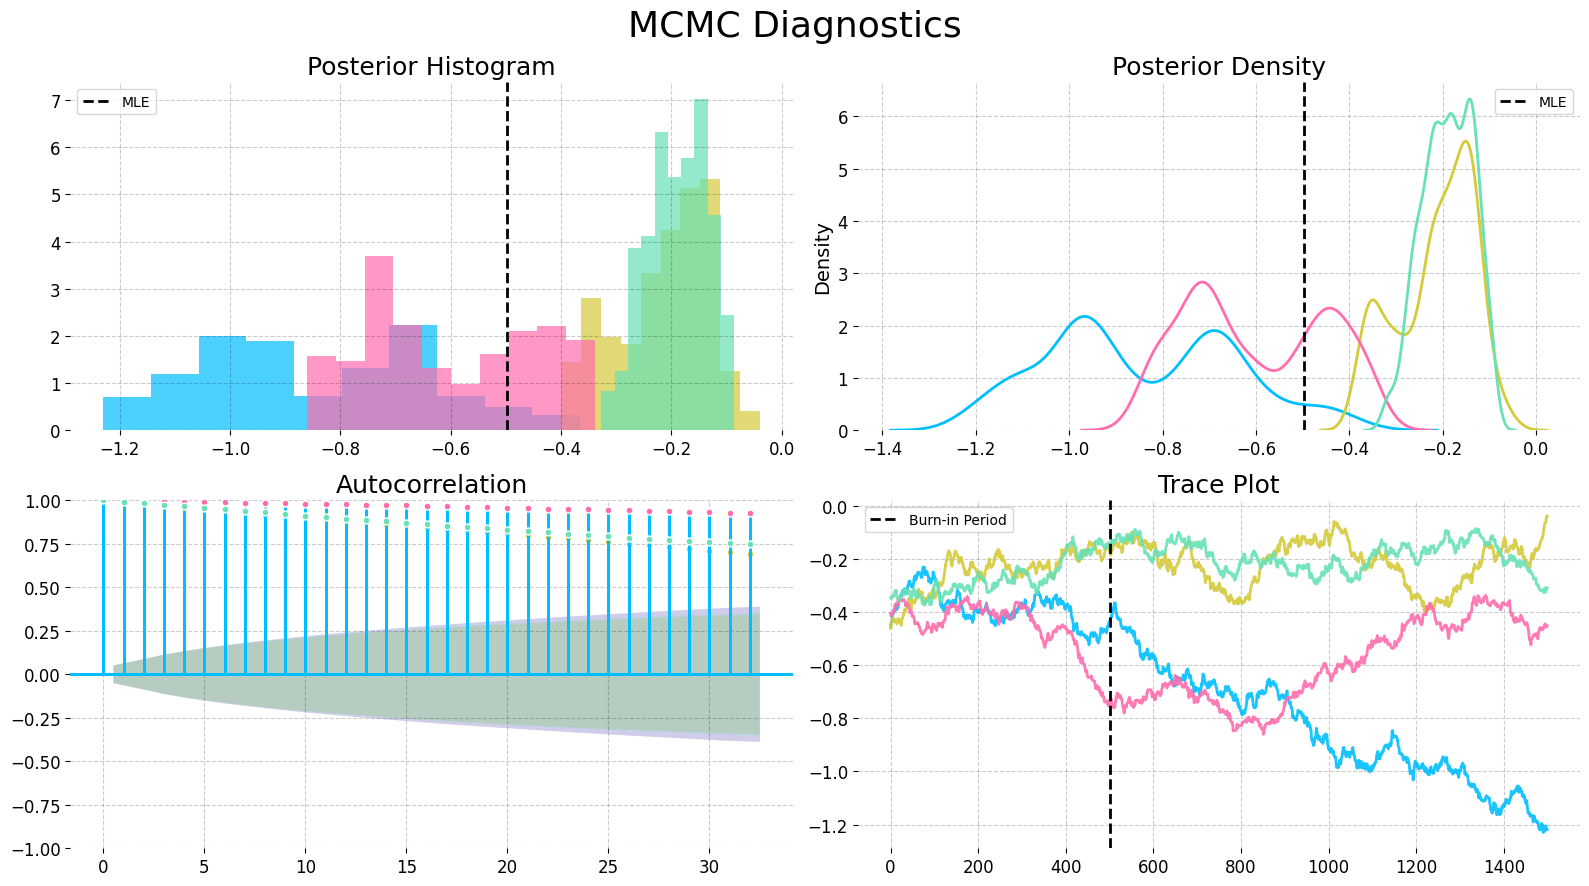
\includegraphics[width=\textwidth/\real{1.25}]{../imgs/pmcmc/mh.png}
    \caption{Convergence diagnostics for the Metropolis-Hastings variant particle MCMC with the random walk proposal and an informative empirical prior from IF2. Here, we display the results for the trend parameter in the Dhaka cholera model of \cite{king08}.}
    \label{fig:mh}
\end{figure}


\begin{figure}[H]
    \centering
    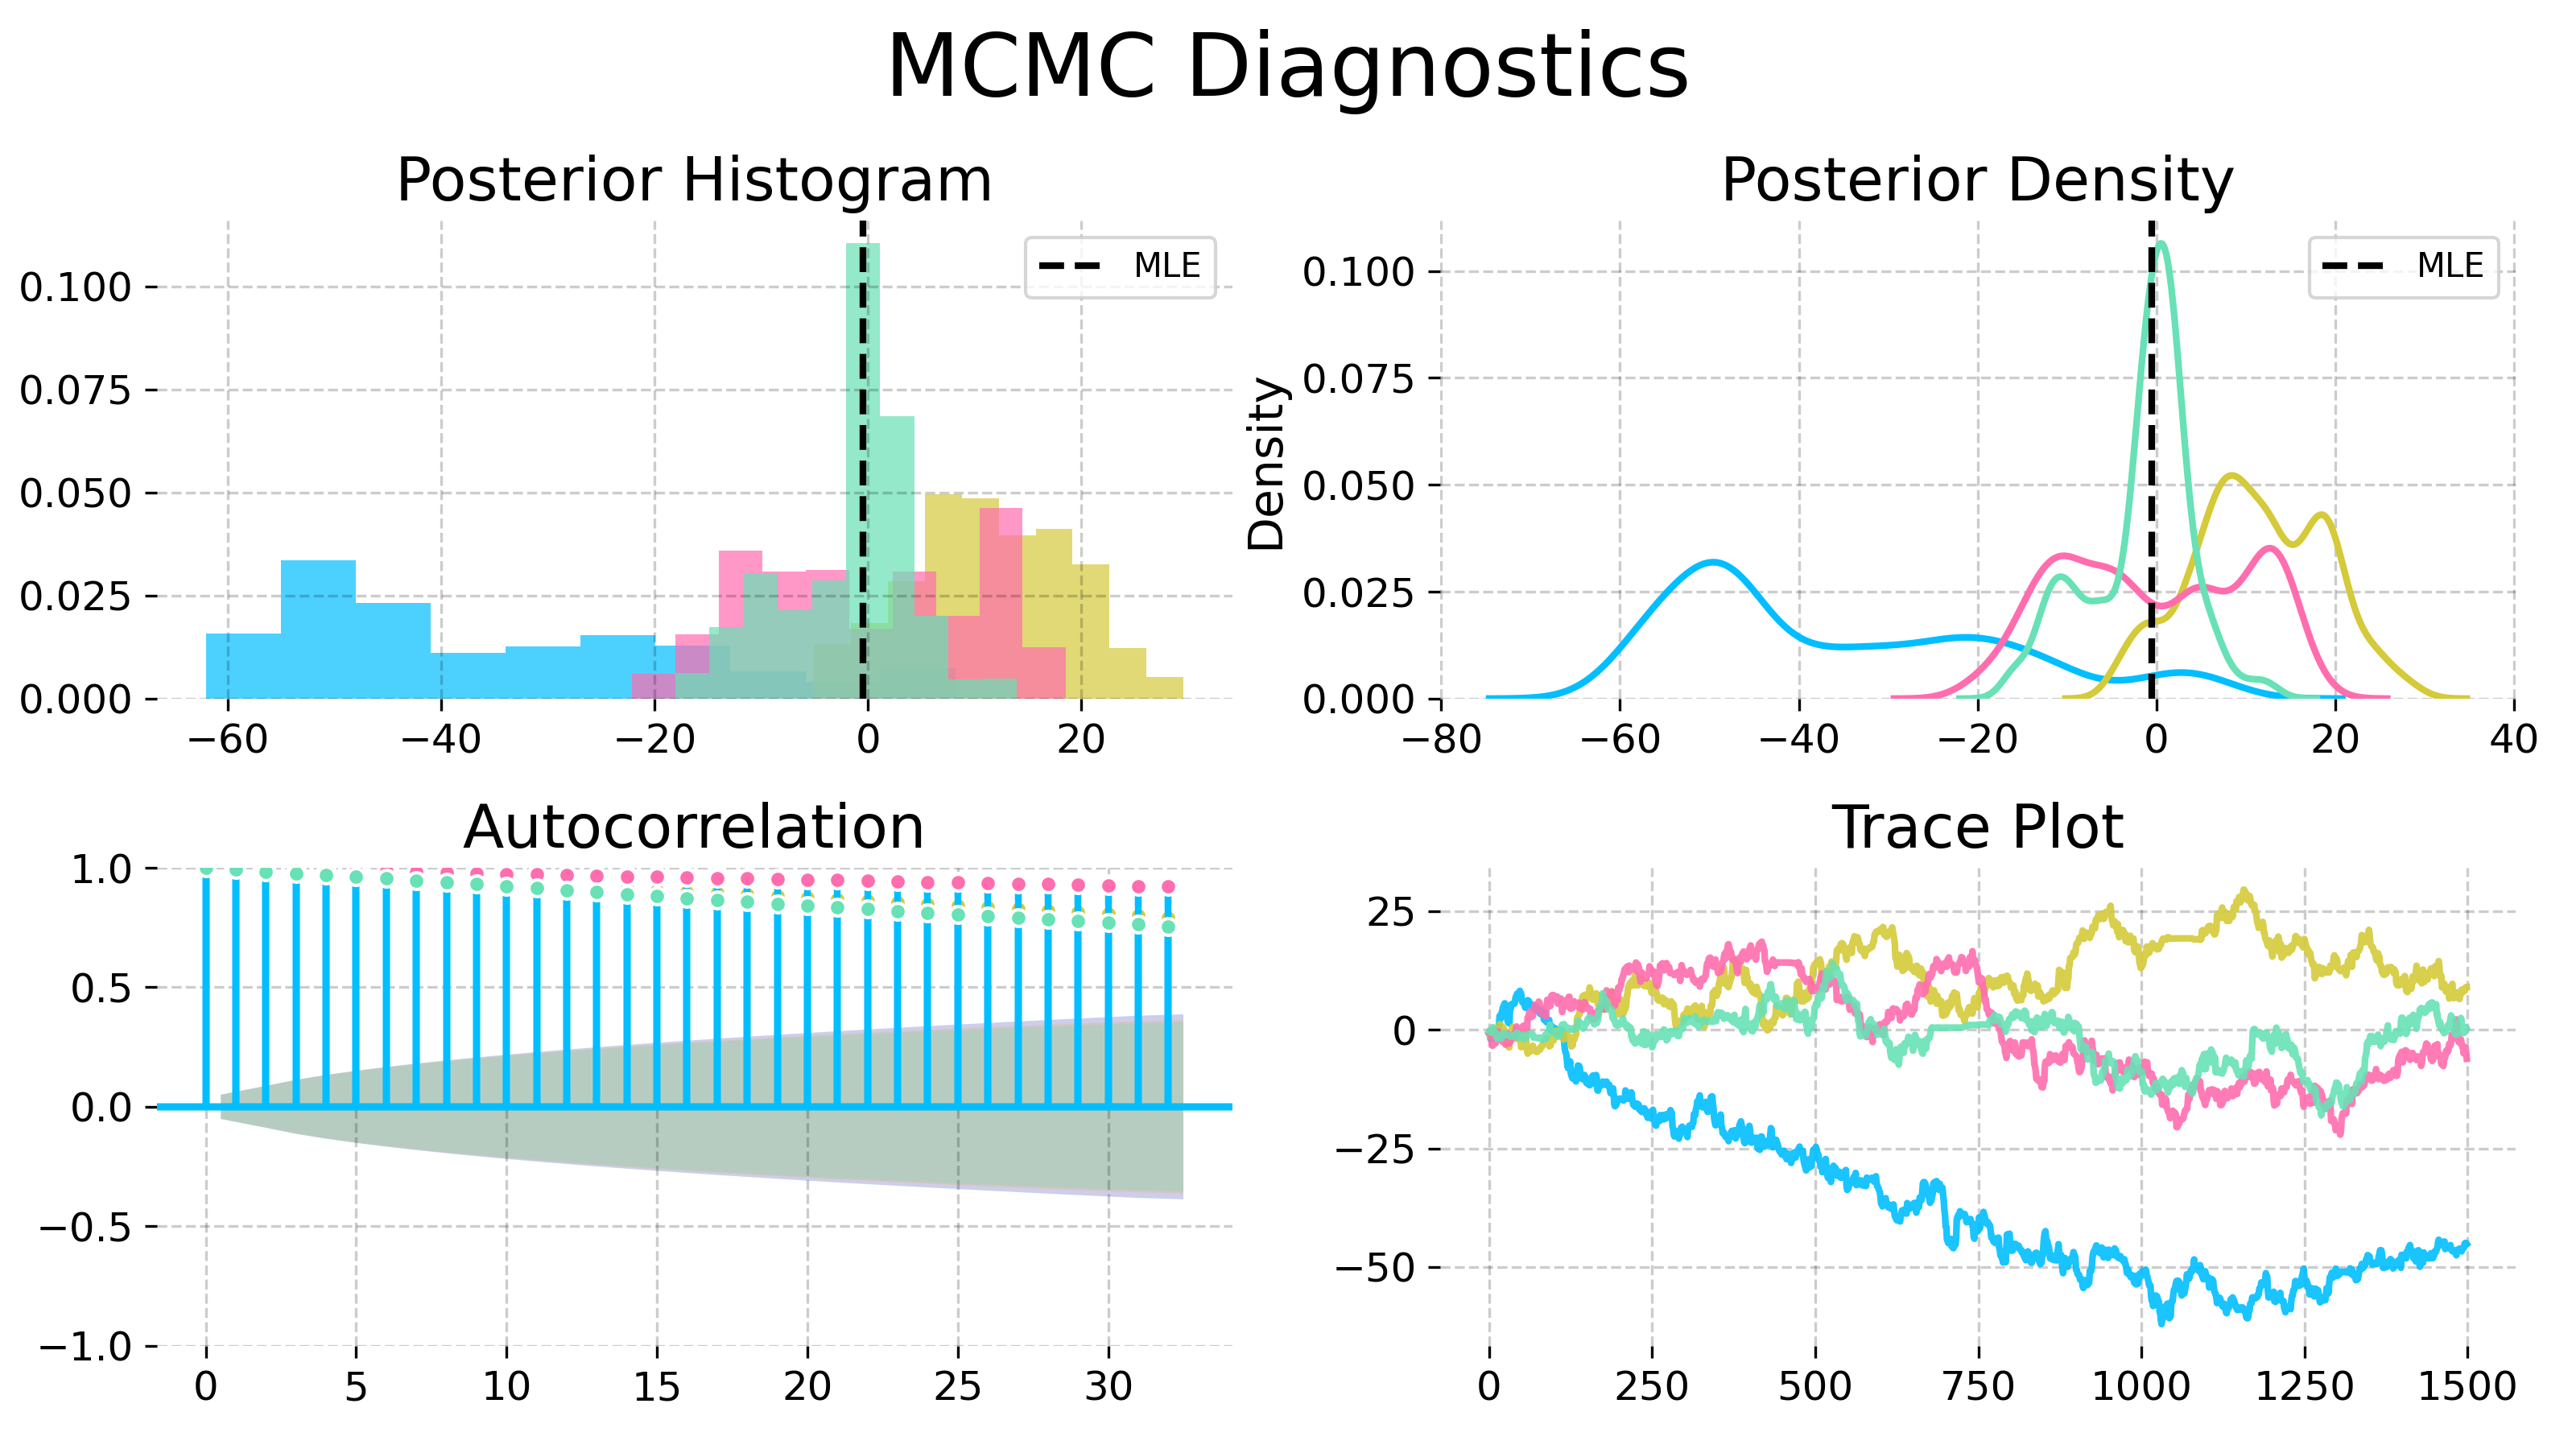
\includegraphics[width=\textwidth/\real{1.1}]{../imgs/pmcmc/nuts.png}
    \caption{Convergence diagnostics for a No-U-Turn Sampler (NUTS) with uniform priors on a compact set. Again, we display the results for the trend parameter in the Dhaka cholera model of \cite{king08}. The NUTS sampler explores more of the posterior than the Metropolis-Hastings sampler, but fails to converge quickly.}
    \label{fig:nuts}
\end{figure}


\begin{figure}[H]
    \centering
    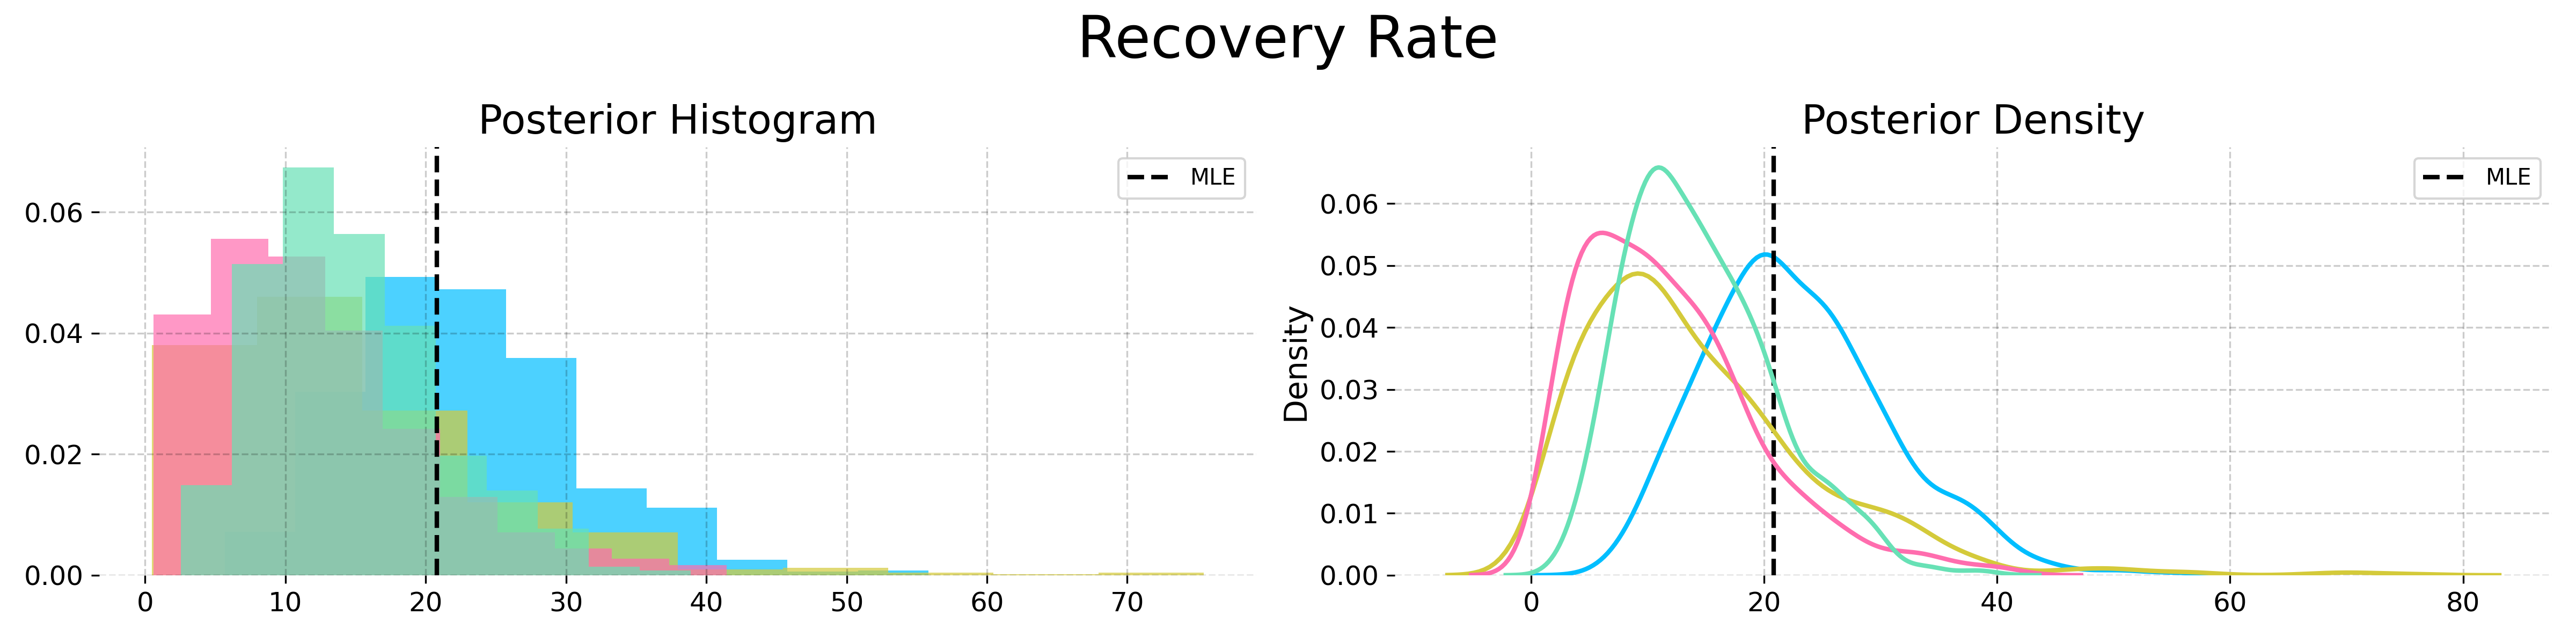
\includegraphics[scale=0.33]{../imgs/pmcmc/nuts_eb/Recovery Rate.png}
    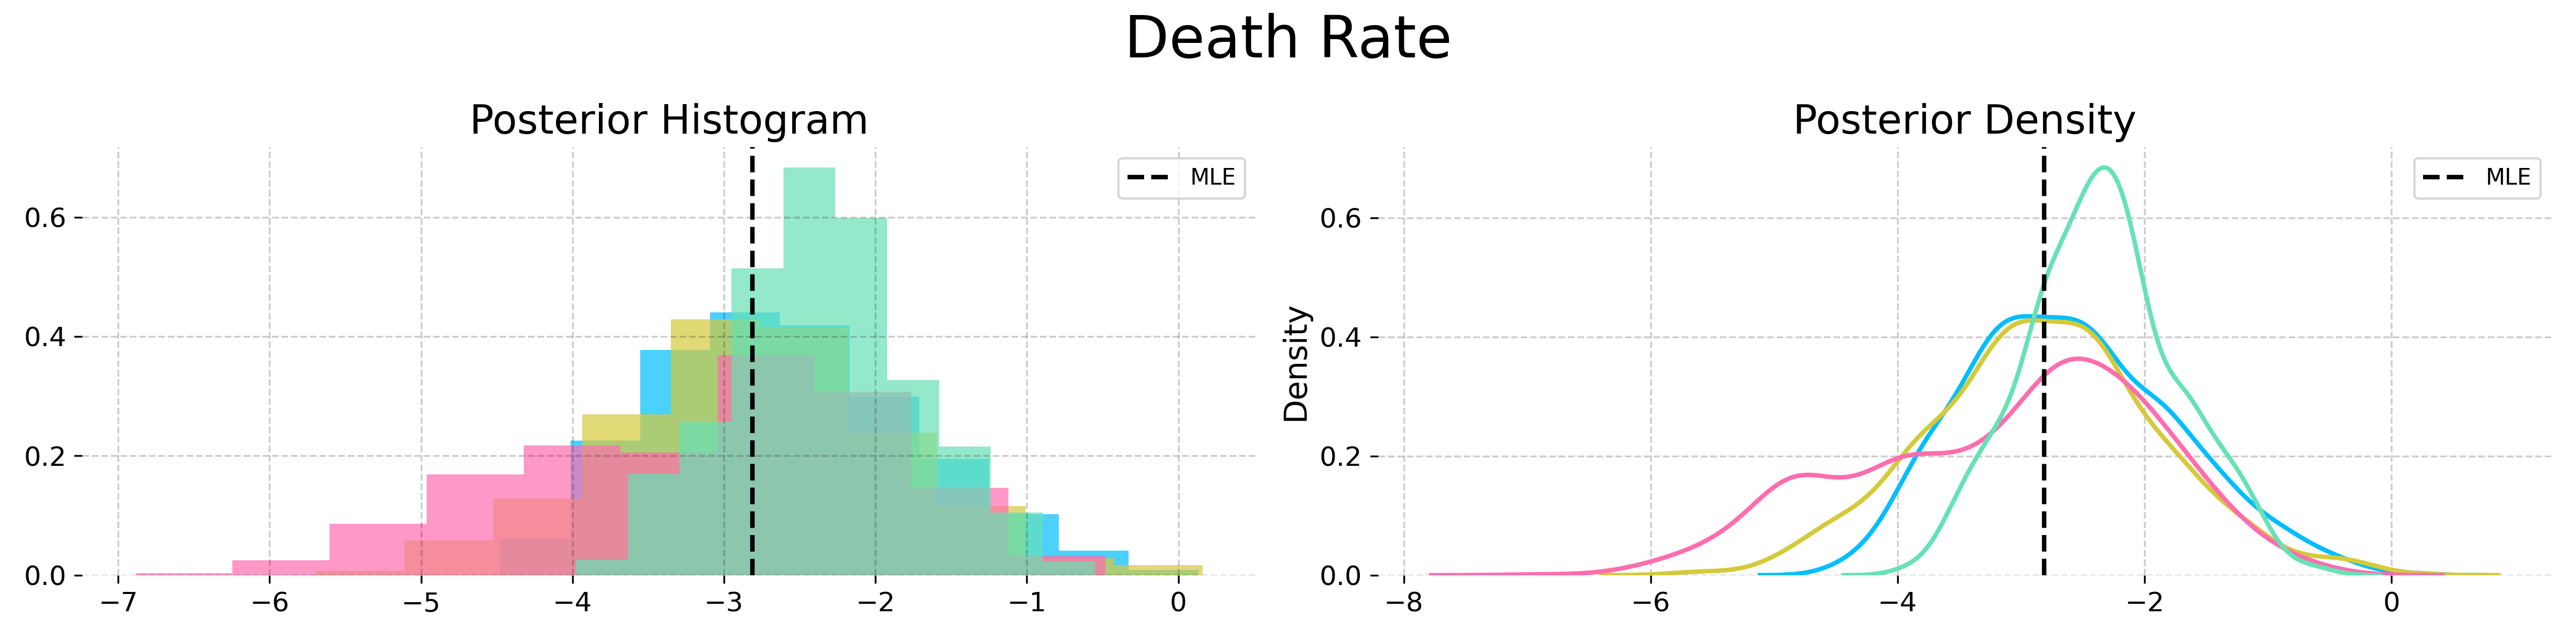
\includegraphics[scale=0.33]{../imgs/pmcmc/nuts_eb/Death Rate.png}
    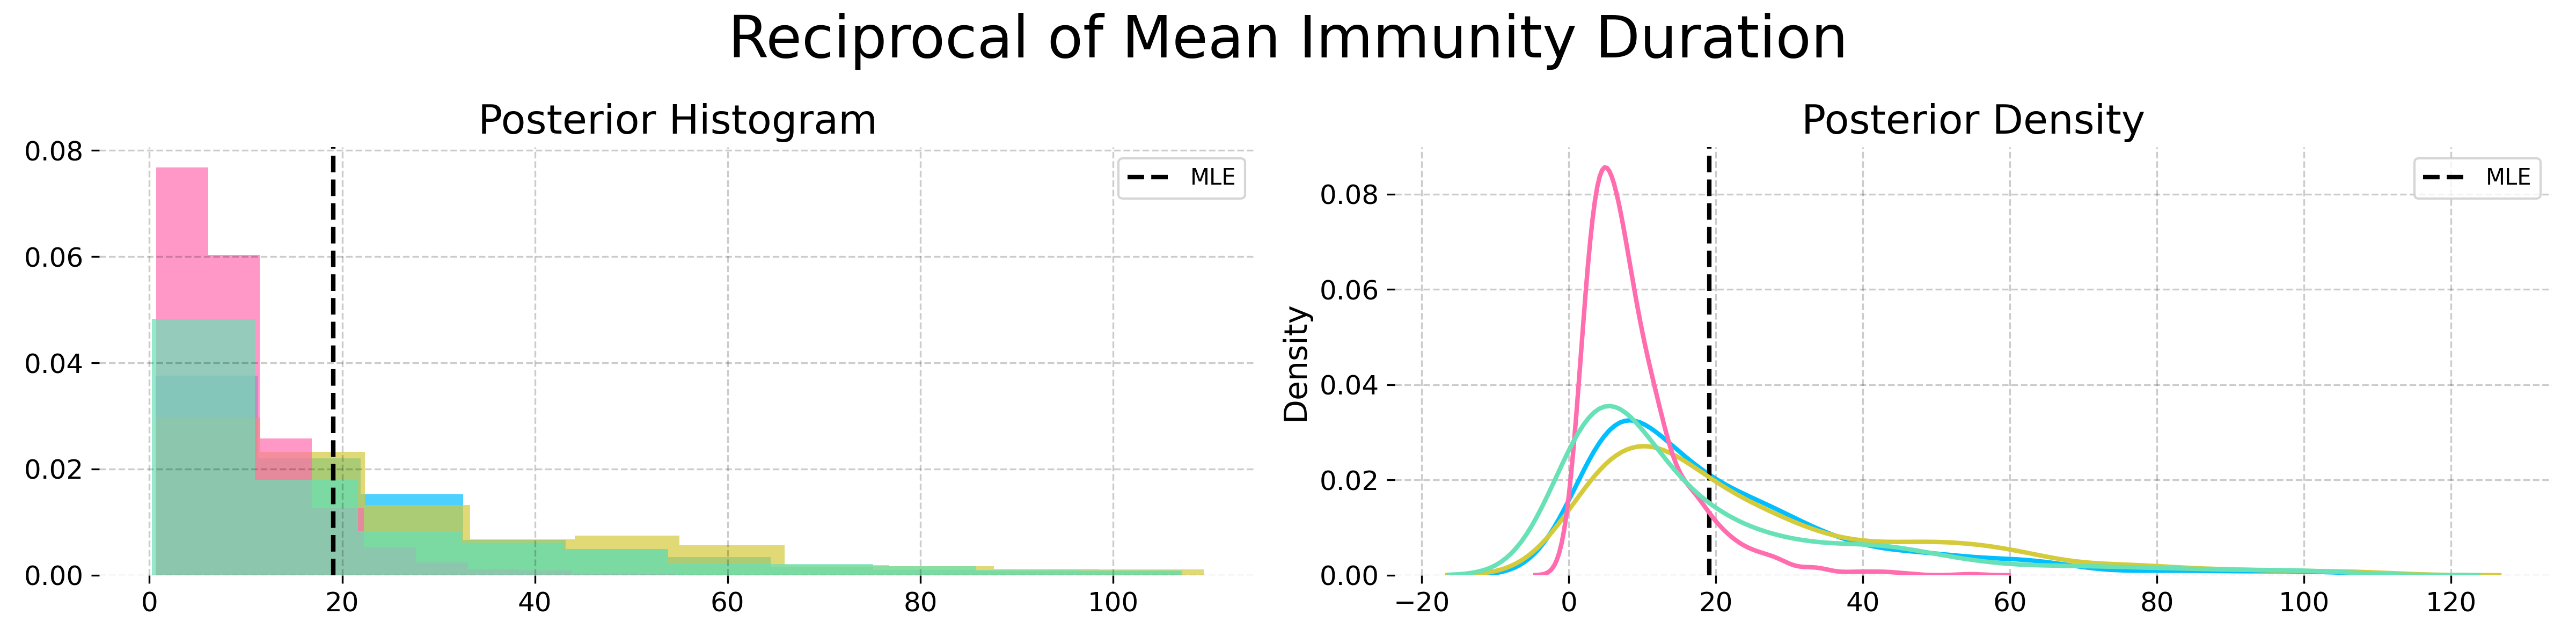
\includegraphics[scale=0.33]{../imgs/pmcmc/nuts_eb/Reciprocal of Mean Immunity Duration.png}
    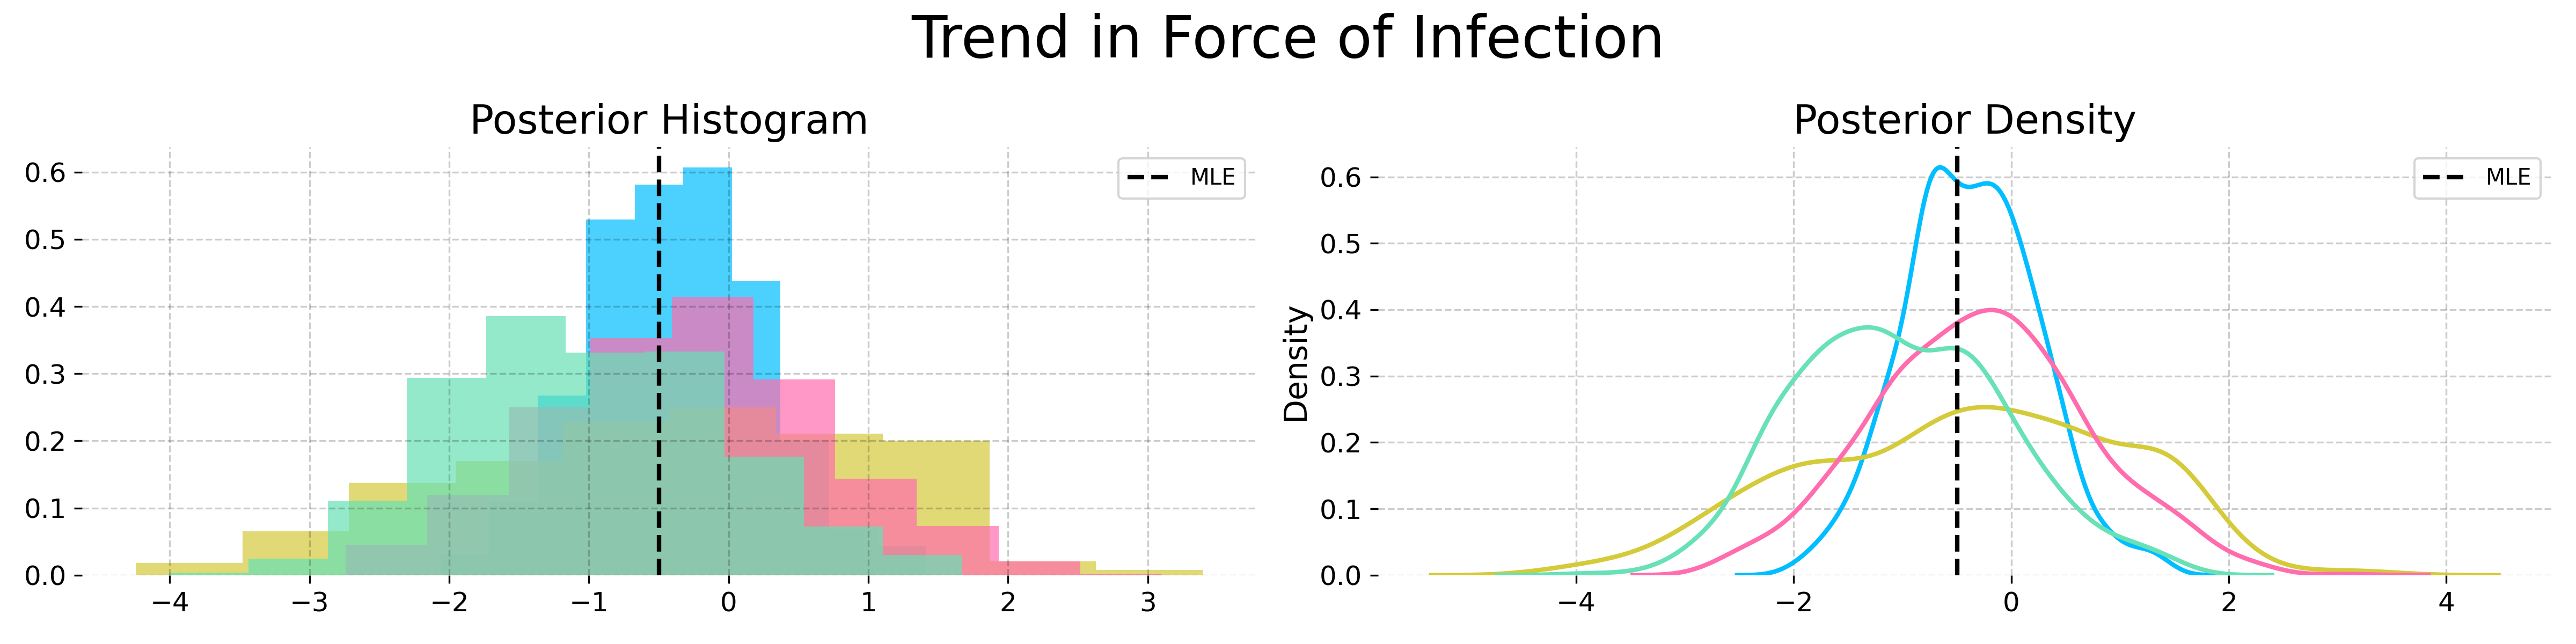
\includegraphics[scale=0.33]{../imgs/pmcmc/nuts_eb/Trend in Force of Infection.png}
    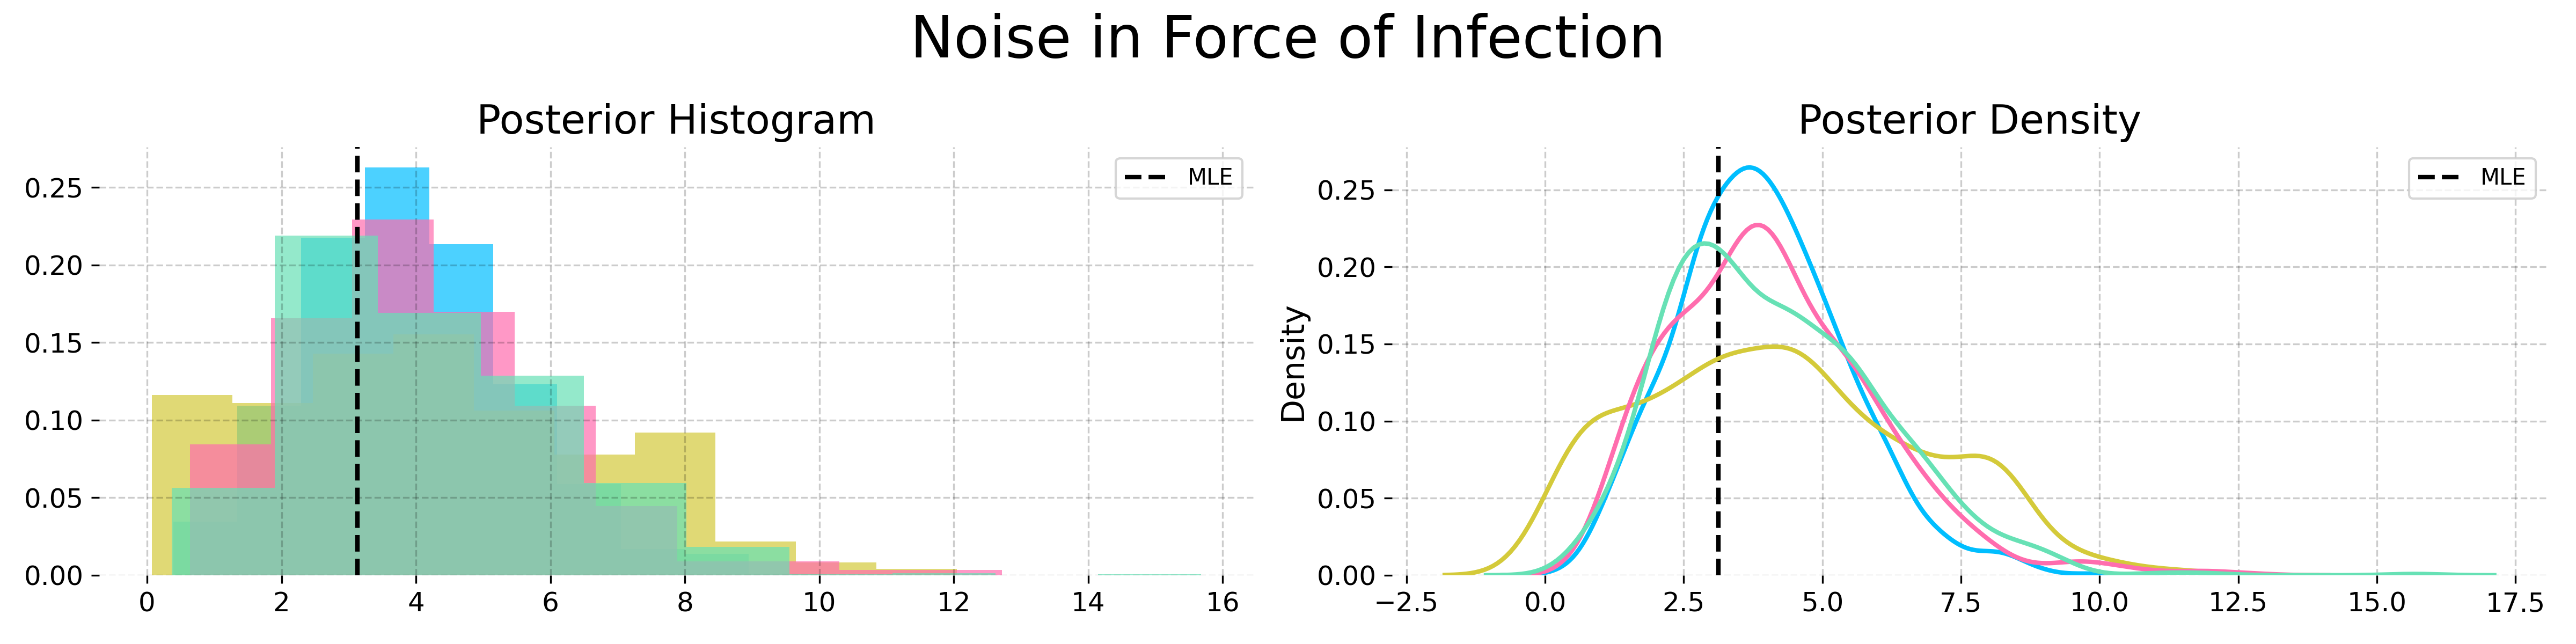
\includegraphics[scale=0.33]{../imgs/pmcmc/nuts_eb/Noise in Force of Infection.png}
    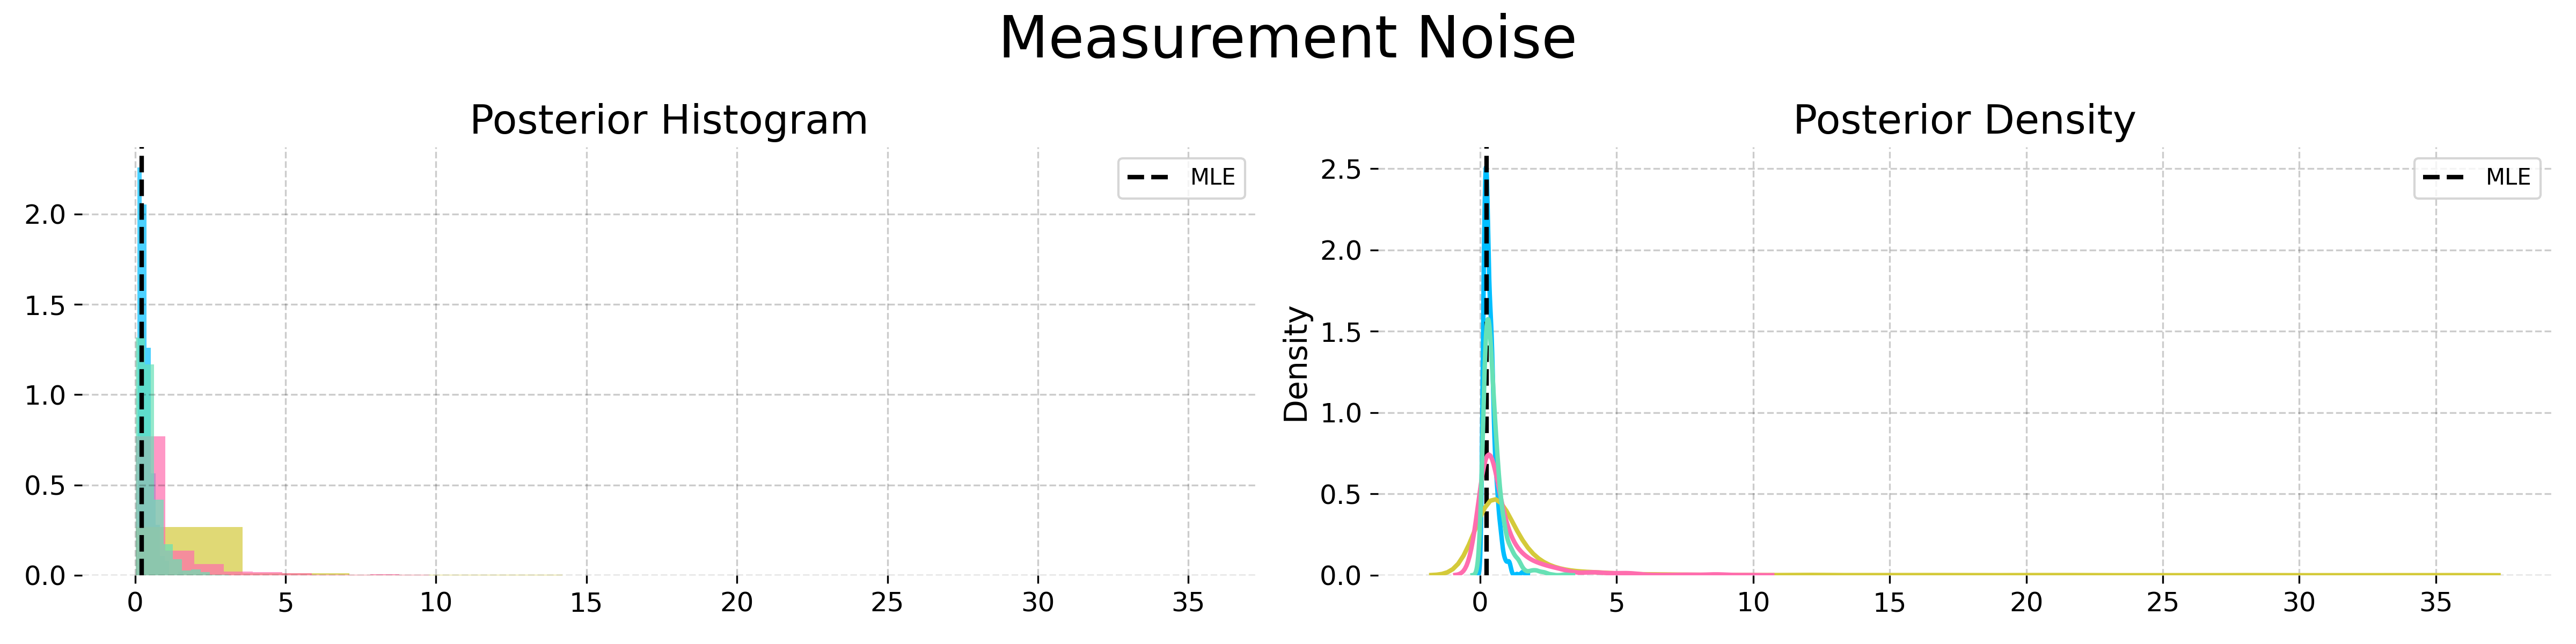
\includegraphics[scale=0.33]{../imgs/pmcmc/nuts_eb/Measurement Noise.png}
    \caption{Posterior estimates from NUTS powered by MOP-$\alpha$ with the informative nonparametric empirical prior obtained from a kernel density estimator on the IF2 parameter cloud. The posterior estimates from each chain are largely in agreement.}
    \label{fig:posteriors}
\end{figure}




}{
}


\end{document}
